%% Preambule - Preamble %% =================================================================================
%            _______                                              __                  __           
%           /       \                                            /  |                /  |          
%           $$$$$$$  | ______    ______    ______   _____  ____  $$ |____   __    __ $$ |  ______  
%           $$ |__$$ |/      \  /      \  /      \ /     \/    \ $$      \ /  |  /  |$$ | /      \ 
%           $$    $$//$$$$$$  |/$$$$$$  | $$$$$$  |$$$$$$ $$$$  |$$$$$$$  |$$ |  $$ |$$ |/$$$$$$  |
%           $$$$$$$/ $$ |  $$/ $$    $$ | /    $$ |$$ | $$ | $$ |$$ |  $$ |$$ |  $$ |$$ |$$    $$ |
%           $$ |     $$ |      $$$$$$$$/ /$$$$$$$ |$$ | $$ | $$ |$$ |__$$ |$$ \__$$ |$$ |$$$$$$$$/ 
%           $$ |     $$ |      $$       |$$    $$ |$$ | $$ | $$ |$$    $$/ $$    $$/ $$ |$$       |
%           $$/      $$/        $$$$$$$/  $$$$$$$/ $$/  $$/  $$/ $$$$$$$/   $$$$$$/  $$/  $$$$$$$/ 
%% Preambule - Preamble %% =================================================================================
\documentclass{assignment}
\coursetitle{Python for AI - Report}
\courselabel{YT0819}
\exercisesheet{Report}{Celik E.}
\student{Celik Ennis}
\university{Thomas More Mechelen-Antwerp - Campus De Nayer}
\school{Departement Electronics ICT - Applied Artificial Intelligence }
\semester{Semester 2, 2025}
\date{\today}

%% Packages =================================================================================================
\usepackage{listings}
\renewcommand{\lstlistlistingname}{Summary}
\usepackage{xcolor} 
\usepackage{amsmath}
\usepackage{pgfplots}
\usepgfplotslibrary{statistics}
\pgfplotsset{compat=1.18,width=10cm}
\usepackage{color}
\usepackage{tcolorbox}
\usepackage{geometry}
\usepackage{array}
\usepackage[utf8]{inputenc}
\usepackage{bookmark}
%% pass hyphens option to url package to allow line breaks at hyphens
%% url package is loaded by hyperref package
\PassOptionsToPackage{hyphens}{url}
\usepackage{hyperref}
\hypersetup{
    colorlinks=true,
    linkcolor=blue,
    filecolor=magenta,      
    urlcolor=cyan,
}
\usepackage[toctitles]{titlesec}
\usepackage{enumitem}
\usepackage[T1]{fontenc}
\usepackage[linesnumbered,ruled]{algorithm2e}
\usepackage{parskip}

%% Define a common style for tcolorboxes
\newtcolorbox{mycolorbox}[1][]{commonstyle,#1}
\newlength\myboxwidth
\setlength{\myboxwidth}{\dimexpr\textwidth-2\fboxsep}

%% Define colors
\definecolor{codegreen}{rgb}{0,0.6,0}
\definecolor{codegray}{rgb}{0.5,0.5,0.5}
\definecolor{codepurple}{rgb}{0.58,0,0.82}
\definecolor{codered}{rgb}{1, 0.2, 0}
\definecolor{typeColor}{rgb}{0.23, 0.70, 0.57}
\definecolor{functionColor}{rgb}{0.79,0.92,0.498}
\definecolor{variableColor}{rgb}{0.23, 0.70, 0.57}
\definecolor{backcolour}{rgb}{0.9,0.95,0.92}
\definecolor{backcolourshadow}{rgb}{0.2,0.95,0.2}

% changing some colors for href links
\newcommand{\errorhref}[3][blue]{\href{#2}{\color{#1}{#3}}}
% a way to write the norm in a mathematical way
\newcommand{\norm}[1]{\left\lVert#1\right\rVert}

% a way to write nested enumerations
\newcommand{\myitem}[1]{%
    \end{enumerate}
    \begin{mdframed}[hidealllines=true,
                    backgroundcolor=blue!20,
                    leftmargin=0,
                    rightmargin=0,
                    innerleftmargin=0,
                    innerrightmargin=0,
                    skipabove=-3\itemsep,
                    skipbelow=0]
        \begin{enumerate}[resume*,itemsep=0pt,topsep=0pt,]
            \item #1
        \end{enumerate}
    \end{mdframed}
    \begin{enumerate}[resume*]
}

\newcolumntype{P}[1]{>{\centering\arraybackslash}p{#1}}
\geometry{
    a4paper,
    total={170mm,257mm},
    left=20mm,
    top=10mm
}

% Listings =================================================================================================
\lstdefinestyle{mystyle}{
    backgroundcolor=\color{backcolour},   
    commentstyle=\color{codegreen},
    keywordstyle=\color{magenta},
    numberstyle=\tiny\color{codegray},
    stringstyle=\color{codepurple},
    basicstyle=\ttfamily\footnotesize,
    breakatwhitespace=false,         
    breaklines=true,                 
    captionpos=b,                    
    keepspaces=true,                 
    numbers=left,                    
    numbersep=5pt,                  
    showspaces=false,                
    showstringspaces=false,
    showtabs=false,                  
    tabsize=2,
    rulesepcolor=\color{backcolourshadow!20},
    frame=shadowbox, 
}

\lstdefinestyle{pythonstyle}{
    language=Python,
    morekeywords={self,as,assert,async,await,break,class,continue,del,elif,except,finally,from,global,is,lambda,nonlocal,pass,raise,return,try,with,yield},
    keywordstyle=\color{magenta}\bfseries,
    commentstyle=\color{codegreen},
    stringstyle=\color{codepurple},
    identifierstyle=\color{variableColor},
    emph={__init__,__str__,__repr__,__call__,__getitem__,__setitem__,__delitem__,__iter__,__next__,__len__,__contains__,__eq__,__ne__,__lt__,__le__,__gt__,__ge__,__add__,__sub__,__mul__,__truediv__,__floordiv__,__mod__,__pow__,__and__,__or__,__xor__,__lshift__,__rshift__,__enter__,__exit__,super},
    emphstyle=\color{functionColor}\bfseries
}

\lstdefinestyle{independentpython}{
    language=Python,
    backgroundcolor=\color{gray!10},
    basicstyle=\ttfamily\footnotesize,
    keywordstyle=\color{blue}\bfseries,
    commentstyle=\color{codegreen}\itshape,
    stringstyle=\color{orange},
    numberstyle=\tiny\color{codegray},
    identifierstyle=\color{black},
    emph={fit,transform,predict,DataFrame,Series,Pipeline,ColumnTransformer,StandardScaler,SimpleImputer,OneHotEncoder,OrdinalEncoder},
    emphstyle=\color{red!70!black}\bfseries,
    frame=single,
    rulecolor=\color{gray!50},
    breaklines=true,
    showstringspaces=false,
    numbers=left,
    numbersep=6pt,
    tabsize=4,
    captionpos=b
}

\lstdefinestyle{plainText}{
    basicstyle=\ttfamily\fontsize{7}{5}\selectfont,
    backgroundcolor=\color{white},
    showstringspaces=false,
    breaklines=false,
    numbers=none
}

\lstdefinestyle{emptystyle}{
    basicstyle=\ttfamily\small,
    backgroundcolor=\color{white},
    showstringspaces=false,
    breaklines=false,
    numbers=none
}
\lstset{style=mystyle}

%% defines the depth and numbering depth of the TOC
\setcounter{tocdepth}{6}
\setcounter{secnumdepth}{6}

\titleformat{\paragraph}[hang]{\normalfont\normalsize\bfseries}{\theparagraph}{1em}{}
\titlespacing*{\paragraph}{0pt}{3.25ex plus 1ex minus .2ex}{0.5em}


% Begin Document ========================================================================================
%
%        _______                       __                  _______    ______    ______  
%       /       \                     /  |                /       \  /      \  /      \ 
%       $$$$$$$  |  ______    ______  $$/  _______        $$$$$$$  |/$$$$$$  |/$$$$$$  |
%       $$ |__$$ | /      \  /      \ /  |/       \       $$ |  $$ |$$ |  $$ |$$ |  $$/ 
%       $$    $$< /$$$$$$  |/$$$$$$  |$$ |$$$$$$$  |      $$ |  $$ |$$ |  $$ |$$ |      
%       $$$$$$$  |$$    $$ |$$ |  $$ |$$ |$$ |  $$ |      $$ |  $$ |$$ |  $$ |$$ |   __ 
%       $$ |__$$ |$$$$$$$$/ $$ \__$$ |$$ |$$ |  $$ |      $$ |__$$ |$$ \__$$ |$$ \__/  |
%       $$    $$/ $$       |$$    $$ |$$ |$$ |  $$ |      $$    $$/ $$    $$/ $$    $$/ 
%       $$$$$$$/   $$$$$$$/  $$$$$$$ |$$/ $$/   $$/       $$$$$$$/   $$$$$$/   $$$$$$/  
%                           /  \__$$ |                                                  
%                           $$    $$/                                                   
%                            $$$$$$/                                                    
% Begin Document ========================================================================================
% This report summarizes the work done in the Python for AI course, 
% focusing on the final project. 
% The project involved implementing a machine learning model to solve/analyze our chosen dataset, 
% utilizing various Python libraries (scikit , tensorflow , pandas , numpy) 
% and techniques learned throughout the course and also AI fund. 
% such as data preprocessing, feature engineering, model training, and evaluation.

\begin{document}
\pagecolor{white!30}
\tableofcontents

% Title Page =========================================================================================
\newpage
\section{Introduction}
\subsection{Course Overview}
The Python for AI course provided a comprehensive introduction to the fundamentals of Python programming, focusing on its applications in artificial intelligence and machine learning. The course covered essential topics such as data manipulation (Pandas), statistical analysis (Matplotlib , Pandas), data-preprocessing (Pandas , Numpy , Scikit-learn) and model training (Tensorflow , Scikit-learn).

\subsection{Final Project Overview}
The final project aimed to apply the knowledge and skills acquired throughout the course to a dataset of choice. 
The project involved selecting a dataset, performing data preprocessing, feature engineering, model training, evaluation and reporting back our results (hence this report). 
The goal was to build a machine learning model that could effectively analyze the dataset and provide meaningful insights.

\subsection{Dataset Selection}
The dataset chosen for the project was the \href{"https://www.kaggle.com/datasets/lainguyn123/student-performance-factors"}{"StudentPerformanceFactors"}
dataset from Kaggle. This dataset contains various factors that may influence student performance, including demographic information, study habits, and academic records. 
\lstinputlisting[style=plainText]{../assets/dataset explained.txt}
My objective is to see/analyze which features/factors influence the students exam score the most.

\subsection{Goal}
My goal for this project is to analyze the dataset and build a machine learning model that can predict the students exam score based on the various factors provided in the dataset.
And to at least achieve a MSE close to 0 with a margin of 0.2 .

% Data Preprocessing =========================================================================================
\newpage
\section{Project}
\subsection{Data Exploration and Preprocessing}
\subsubsection{Exploration}
The first step in the project was to explore and preprocess the dataset. We explore these 2 steps in chapter 1 and 2 of the code.
This involved loading the dataset, examining its structure, and identifying any missing or inconsistent data.
After that, we performed data preprocessing to clean the dataset and prepare it for analysis and pass it on to a ML model.
In this case, the dataset was relatively clean, with a few missing values here and there and some exam scores outside of the normal $[0;100]$ range.
\lstinputlisting[style=plainText,linerange={10-31}]{../chap_1_peering_into_the_data_abyss/part_1_exploration.py}
\lstinputlisting[style=plainText,linerange={36-44}]{../chap_1_peering_into_the_data_abyss/part_1_exploration.py}

As we explore further into dataset by drawing up the correlation matrix, we can see that some features are highly correlated with the exam score, such as the number of hours studied
or the attendance. (the picture below shows the correlation matrix of the dataset keep in mind that the correlation matrix is not a perfect representation of the data, but it gives us a good idea of which features are correlated with the exam score)
\begin{center}
    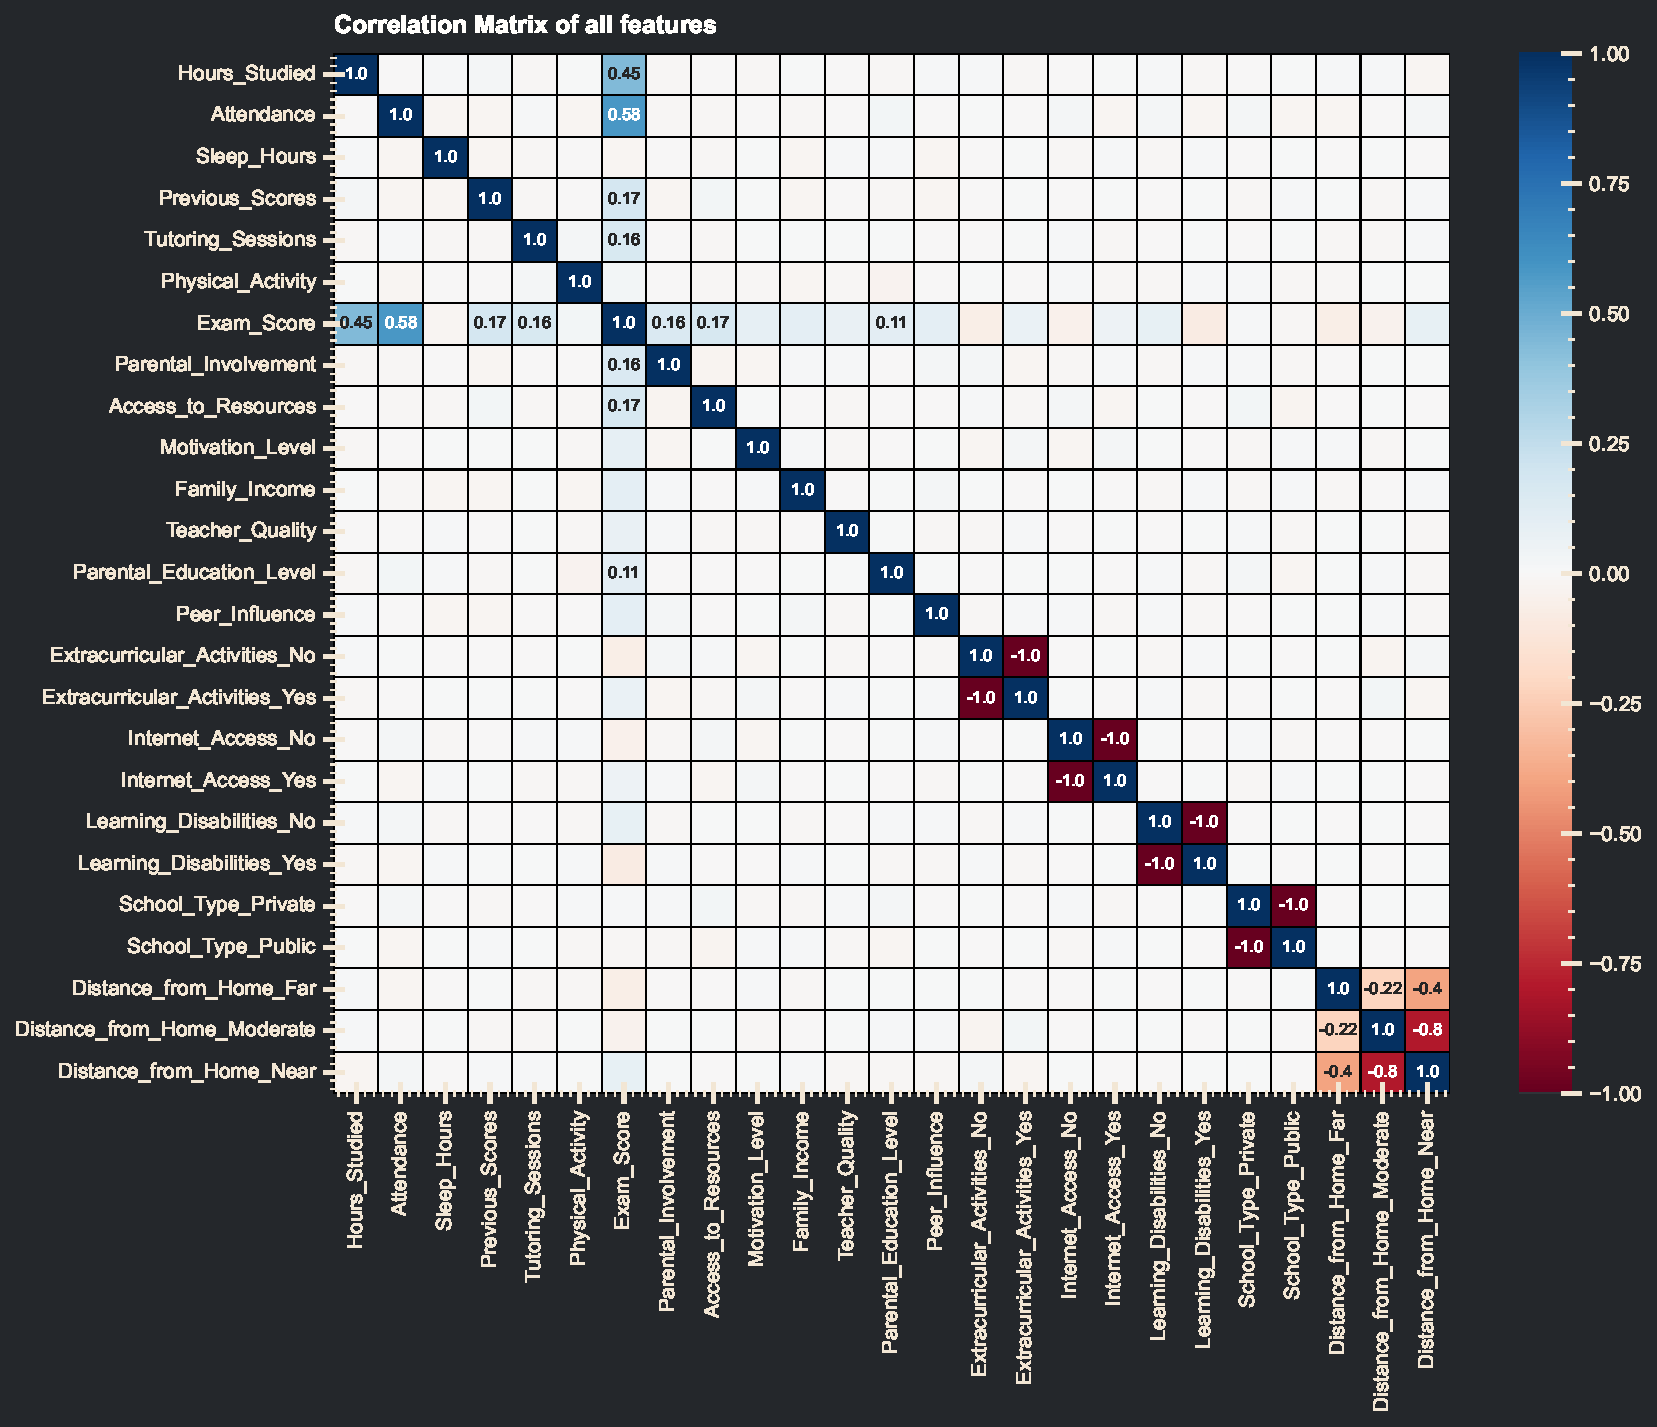
\includegraphics[width=5.5in]{../report/assets/correlation_matrix.pdf}
\end{center}

\begin{center}
    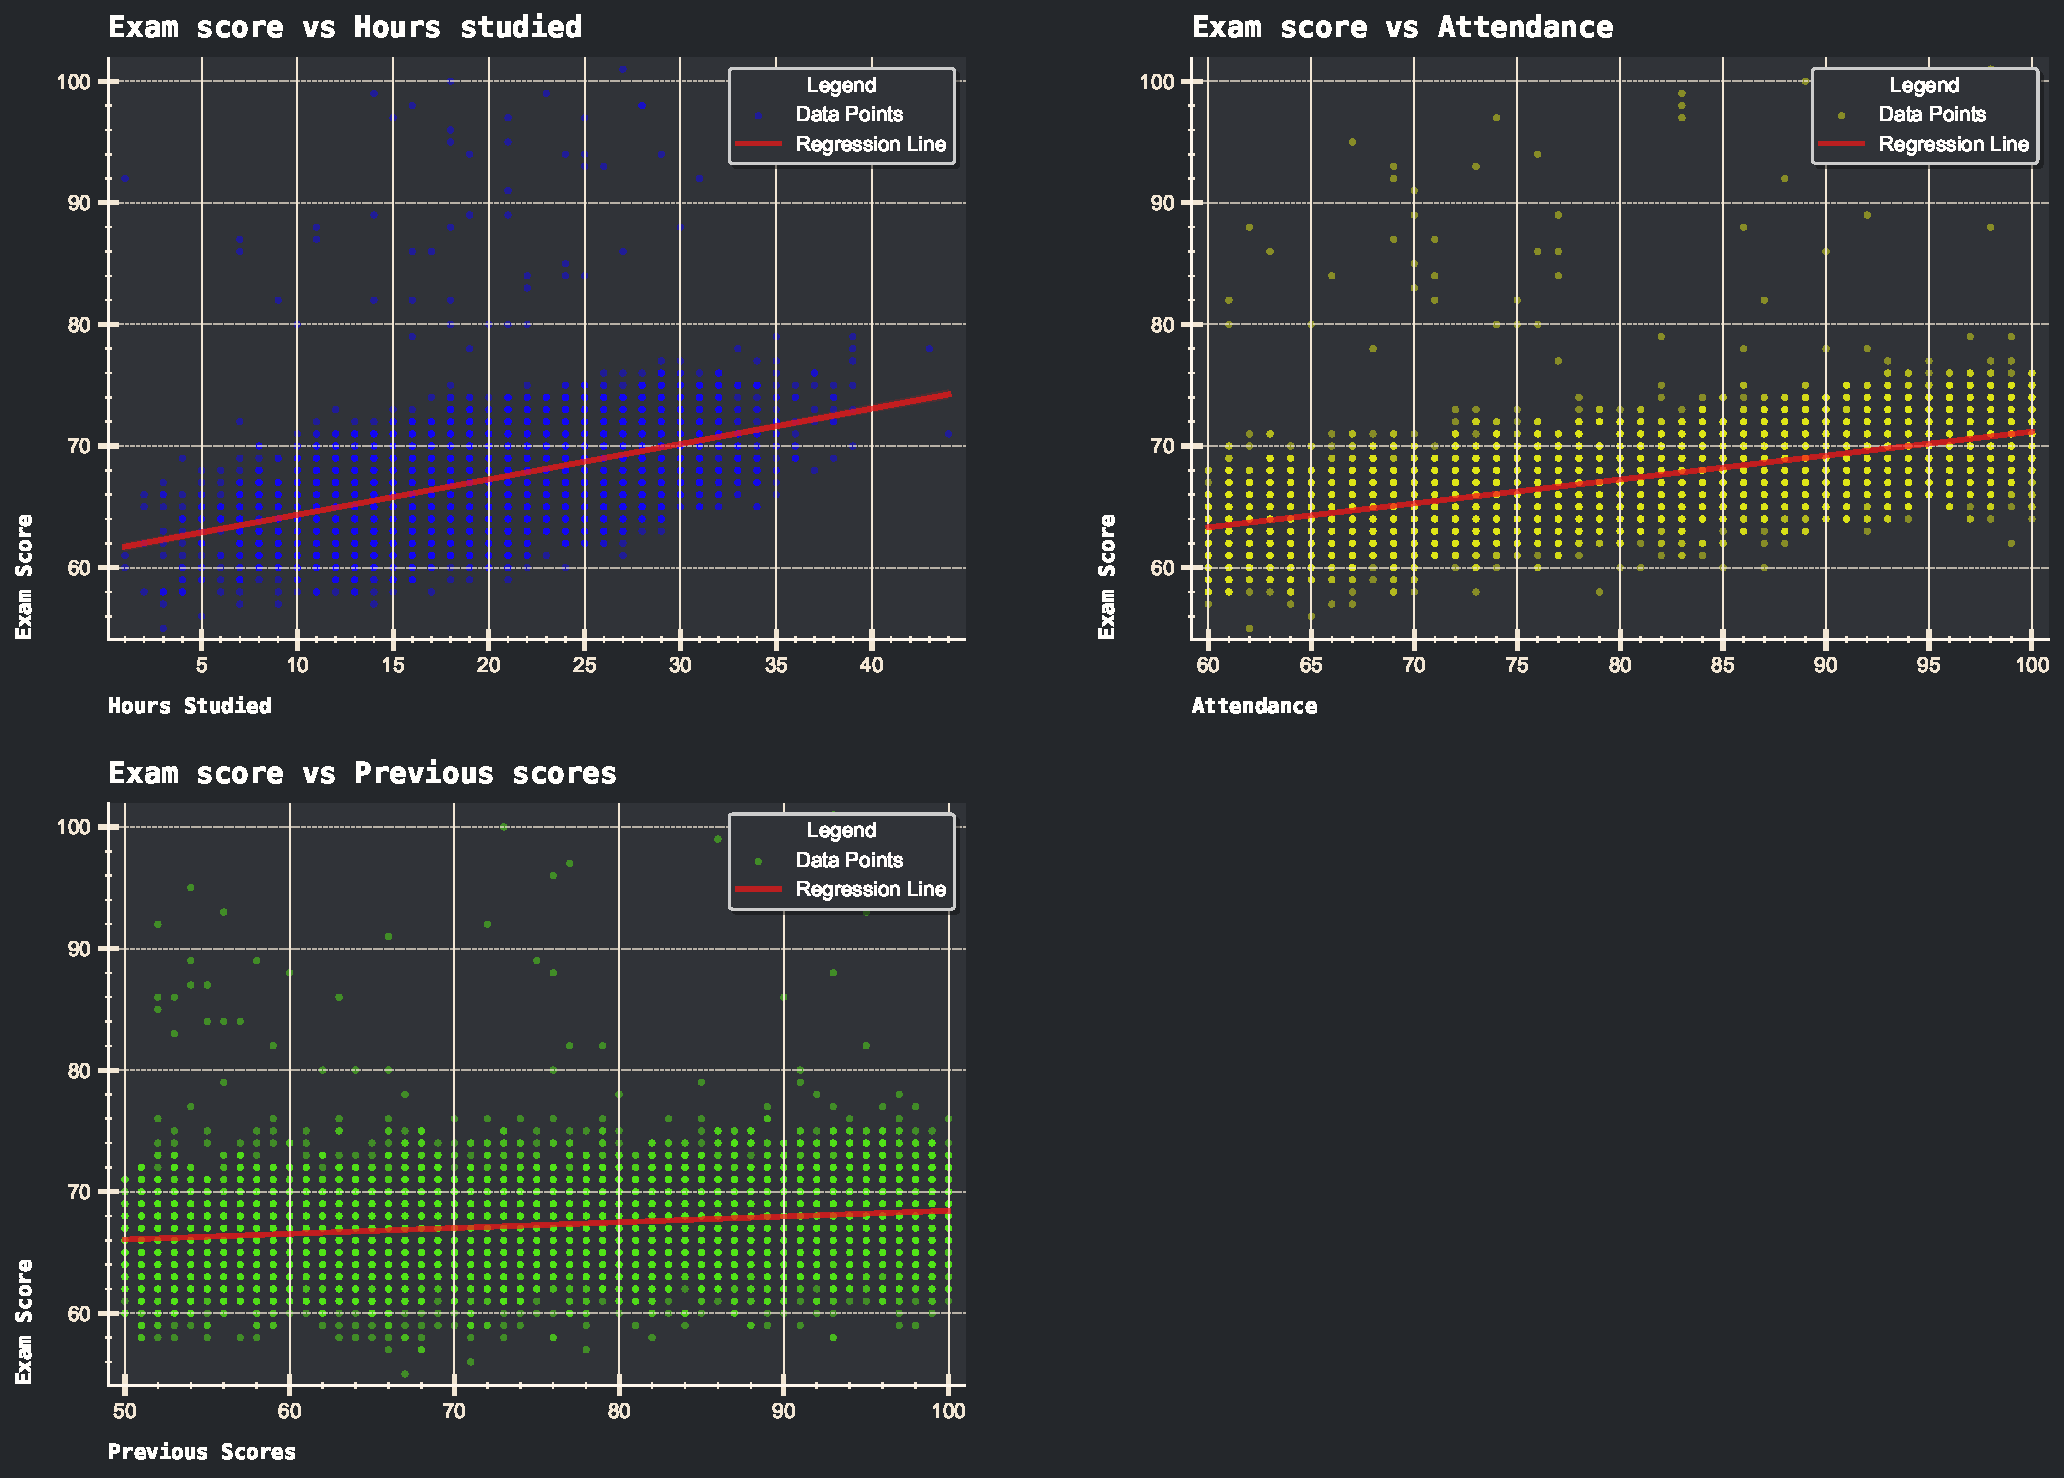
\includegraphics[width=5.5in]{../report/assets/scatter_plots_exploration.pdf}
\end{center}
I did try to create new features:
\begin{enumerate}
    \item Study Efficiency : a combination of the number of hours studied and the attendance rate, to see if students who study more and attend more classes perform better.
    \item Preparation : a combination of tutoring sessions and previous exam scores, to see if students who have more tutoring sessions and better previous exam scores perform better.
    \item Resource Utilization Score : a combination of Access to Resources, Internet Access and Tutoring sessions to see if students which different eductional resources would perform better.
    \item Health Score : a combination of sleep hours, physical activity to see if students who take care of their health perform better.
    \item Motivation Effort : a combination of motivation and hours studied to see if students who are more motivated and put in more effort perform better.
    \item Parental Support Score : a combination of parental involvement and parental education level to see if students who have more parental support perform better.
\end{enumerate} 
These new features were created to see if they would improve the performance of the model, but in the end they did not improve the performance of the model. As you will see later on.
The correlation matrix however show that some of these features do have some correlation with the exam score, but not enough to make a significant difference in the performance of the model. 
\begin{center}
    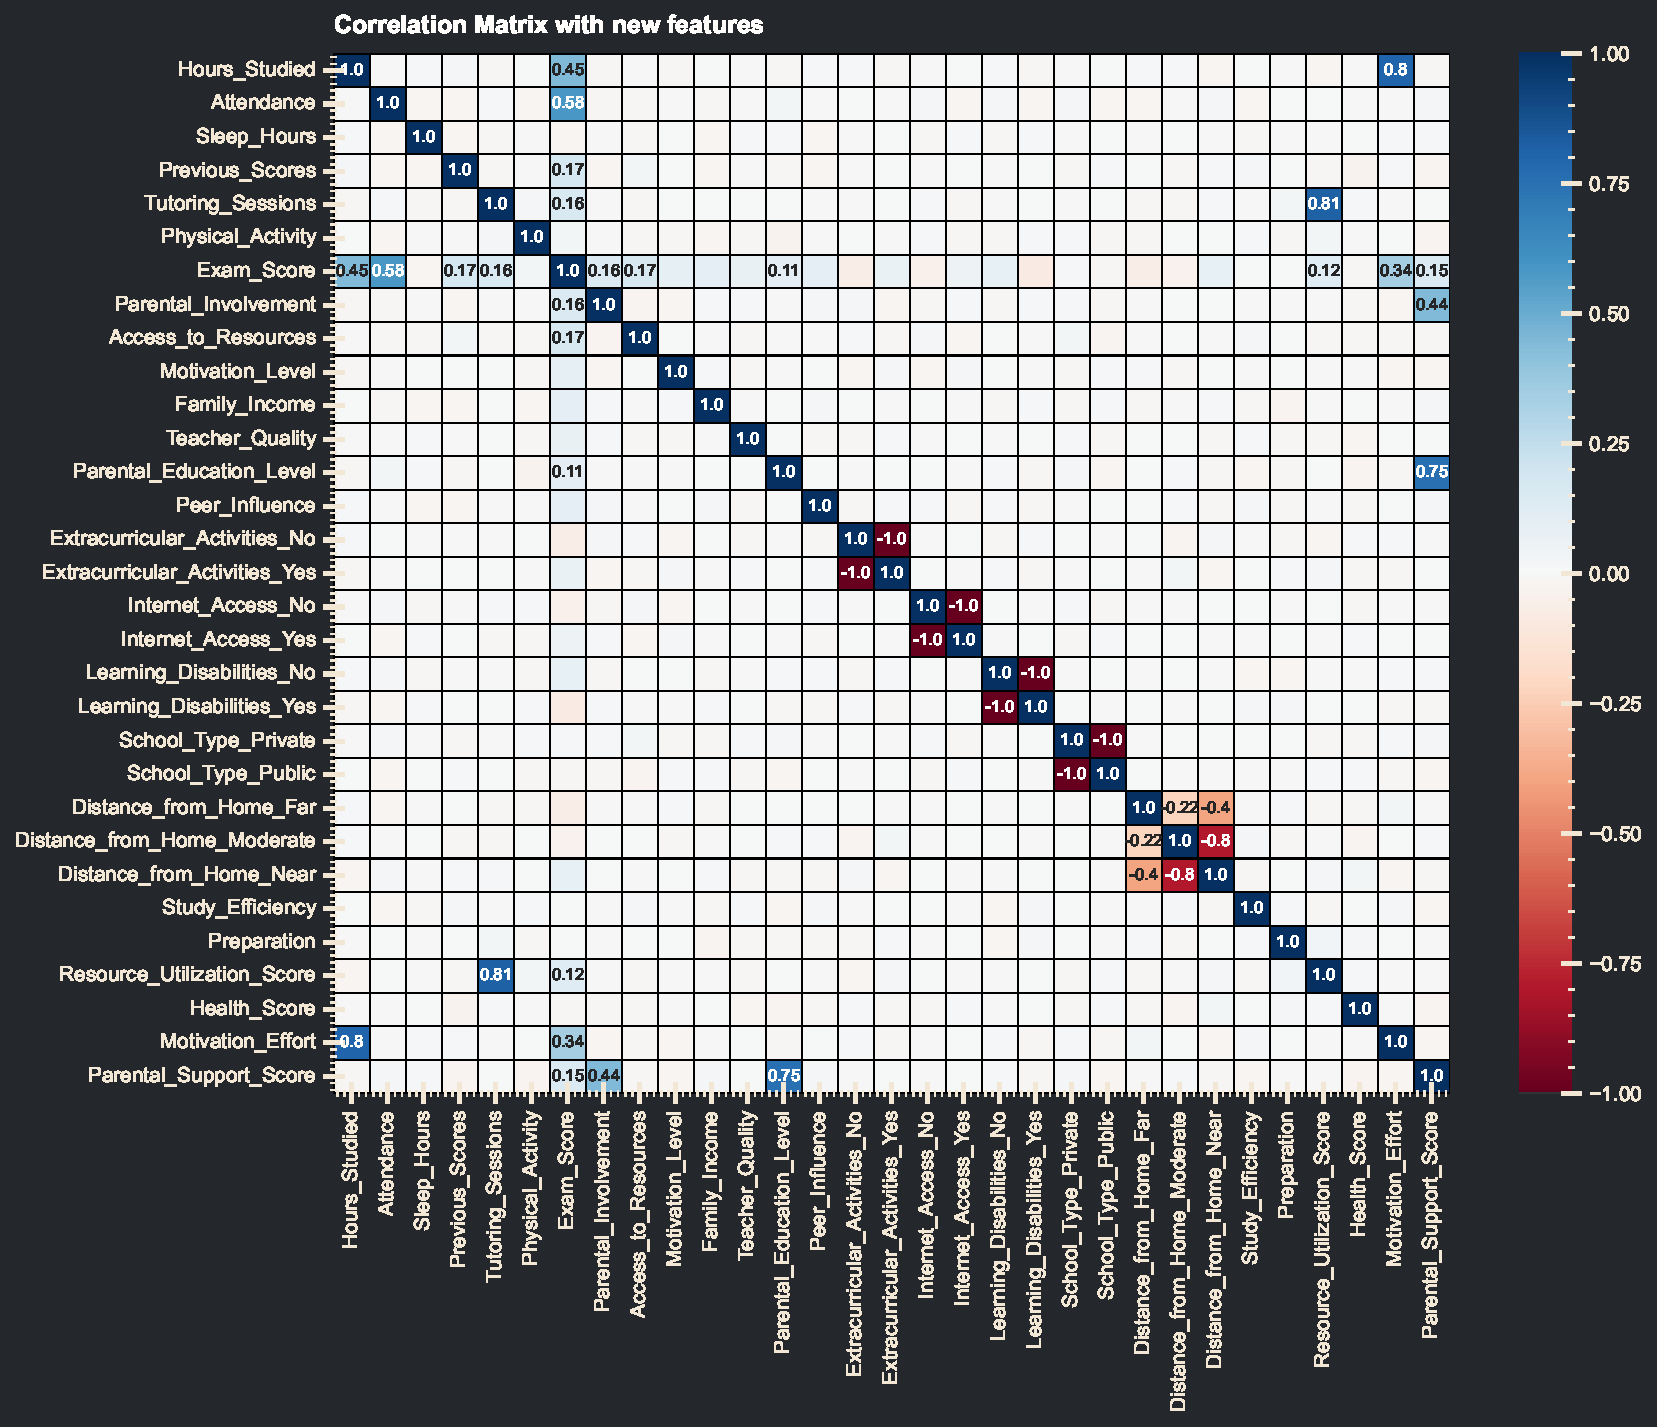
\includegraphics[width=5.5in]{../report/assets/correlation_matrix_new_features.pdf}
\end{center}
Now again keep in the mind the correlation matrix only shows linear correlation, so it is possible that some of these features do have a non-linear correlation with the exam score.

\subsubsection{Preprocessing}
The next step was to preprocess the dataset. This involved handling missing values, encoding categorical variables, and scaling numerical features.
I first cleaned the dataset by removing any rows with missing values and then I encoded the categorical variables using one-hot encoding or ordinal encoding depending on the categorical column.
For example , categories like "yes" and "no" were encoded as 1 and 0 respectively, while categories like "High", "Medium", "Low" were encoded as 4, 3, 2, 1 respectively.
\lstinputlisting[style=plainText,linerange={16-27}]{../chap_1_peering_into_the_data_abyss/part_2_exploration.py}
For numerical features , i used a StandardScaler to scale the features to have a mean of 0 and a standard deviation of 1.
Just to be sure we also use a simple imputer to fill in any missing values with the mean of the column , or the most frequent value.
Putting it all together, inside a Pipeline and a ColumnTransformer to apply the preprocessing steps to the numerical and categorical features.
\lstinputlisting[style=independentpython,language=python,linerange={46-71}]{../chap_2_cleansing_the_noise/part_1_cleaning.py}
We then applied the preprocessing steps to the dataset that has been split it into training and testing sets.
And finally we saved the preprocessed dataset to a CSV file for later use.
Also keeping a copy of the original dataset for reference and saving a test and train dataset with the columns i want to keep.
\lstinputlisting[style=plainText,language=python,linerange={108-117}]{../chap_2_cleansing_the_noise/part_1_cleaning.py}

resulting in this exam score distribution plot:
\begin{center}
    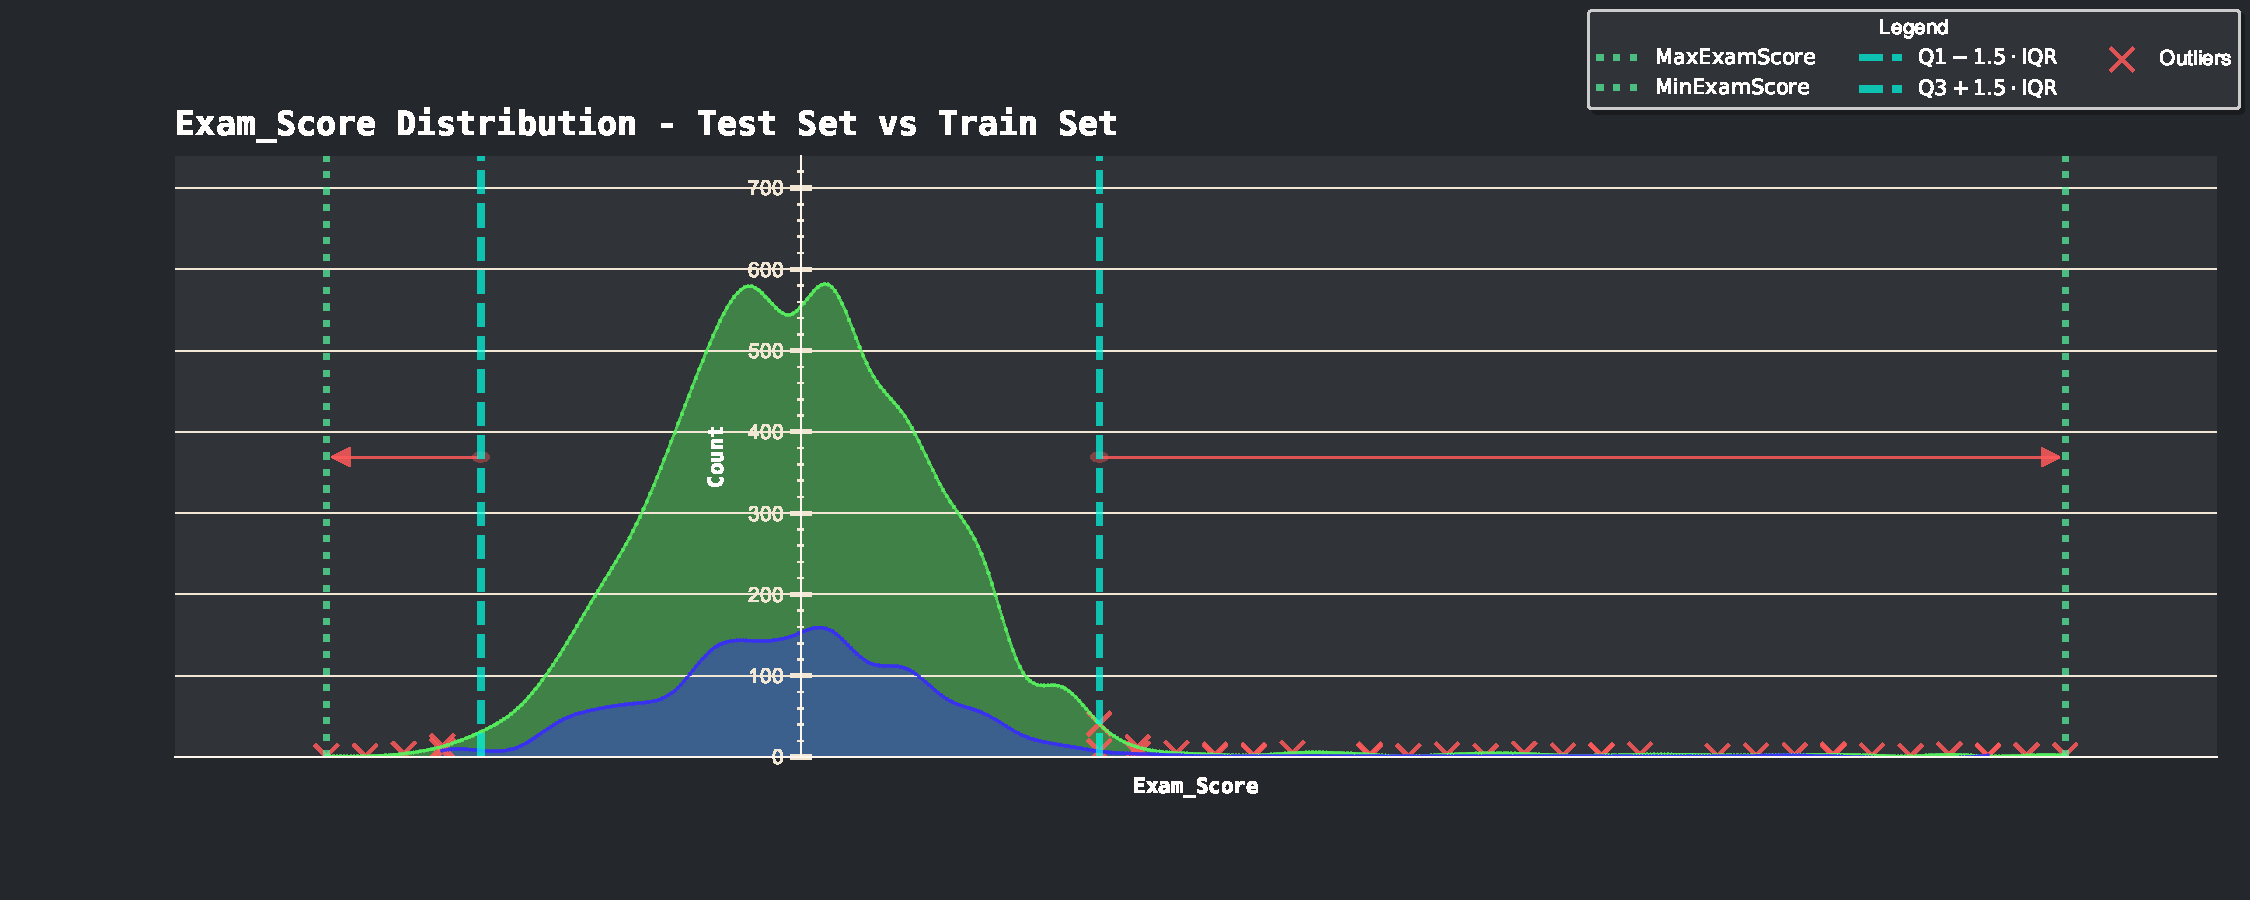
\includegraphics[width=6.5in]{../report/assets/Exam_Score_Distribution_test_vs_train_with_outliers.pdf}
\end{center}

However we can see that the exam score distribution is not normal and has some outliers, which can affect the performance of the model.
So I decided to remove the outliers from the dataset by removing any rows with exam scores outside of the range $[Q1 - 1.5IQR,Q1 + 1.5IQR]$.
resulting in this exam score distribution plot: 
\begin{center}
    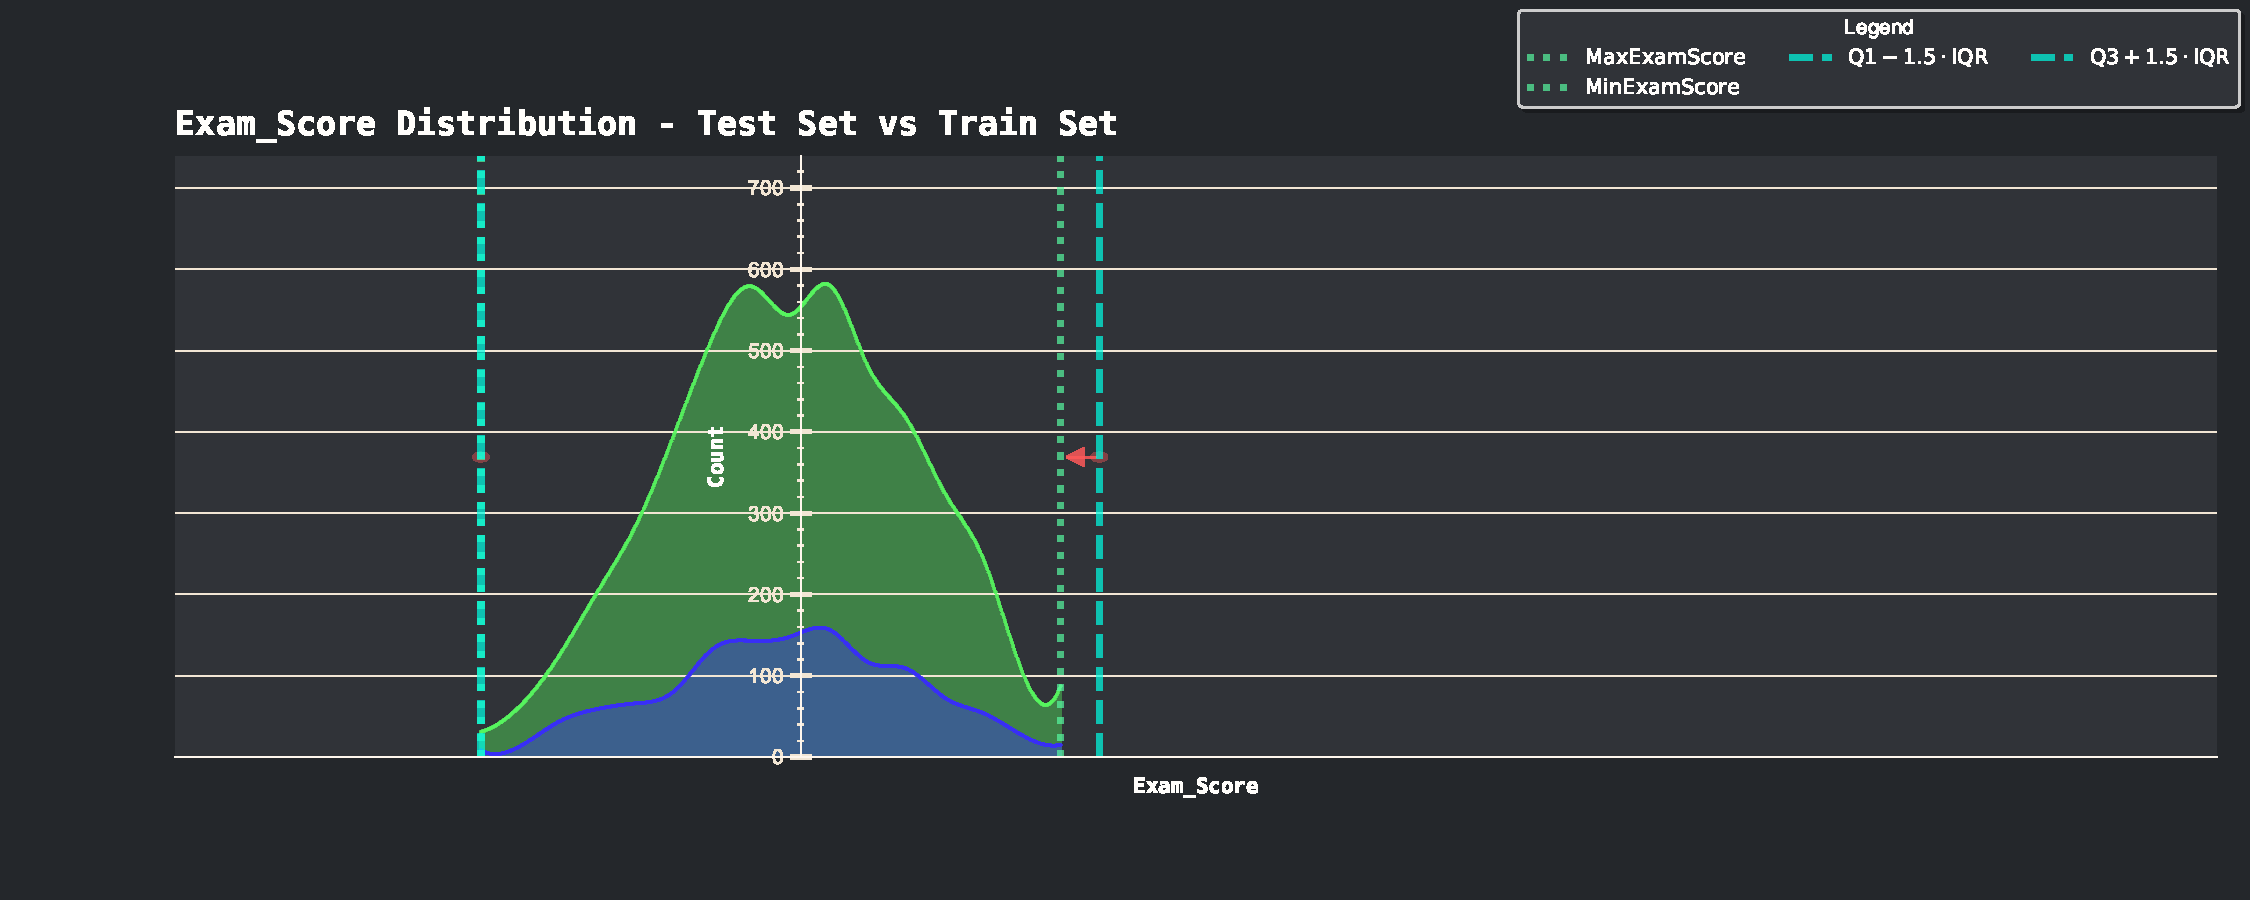
\includegraphics[width=6.5in]{../report/assets/Exam_Score_Distribution_test_vs_train_without_outliers.pdf}
\end{center}

\newpage
\subsection{Searching for models}
\subsubsection{Model Selection}
After preprocessing the dataset, the next step was to select a machine learning model to train on the dataset.
I decided to use a regression model since the goal is to predict the exam score, which is a continuous variable.
I started with a simple linear regression model, and other ML models such as  KNNRegressor,SVR,etc... , which is a good baseline model for regression tasks.
Alongside i used Cross-Validation to evaluate the performance of the model on the training set.
\lstinputlisting[style=independentpython,language=python,linerange={30-42}]{../chap_3_the_hunt_for_the_right_model/part_1_regression.py}

some of these models performed well on the test set, but others did not perform well at all.
\begin{center}
    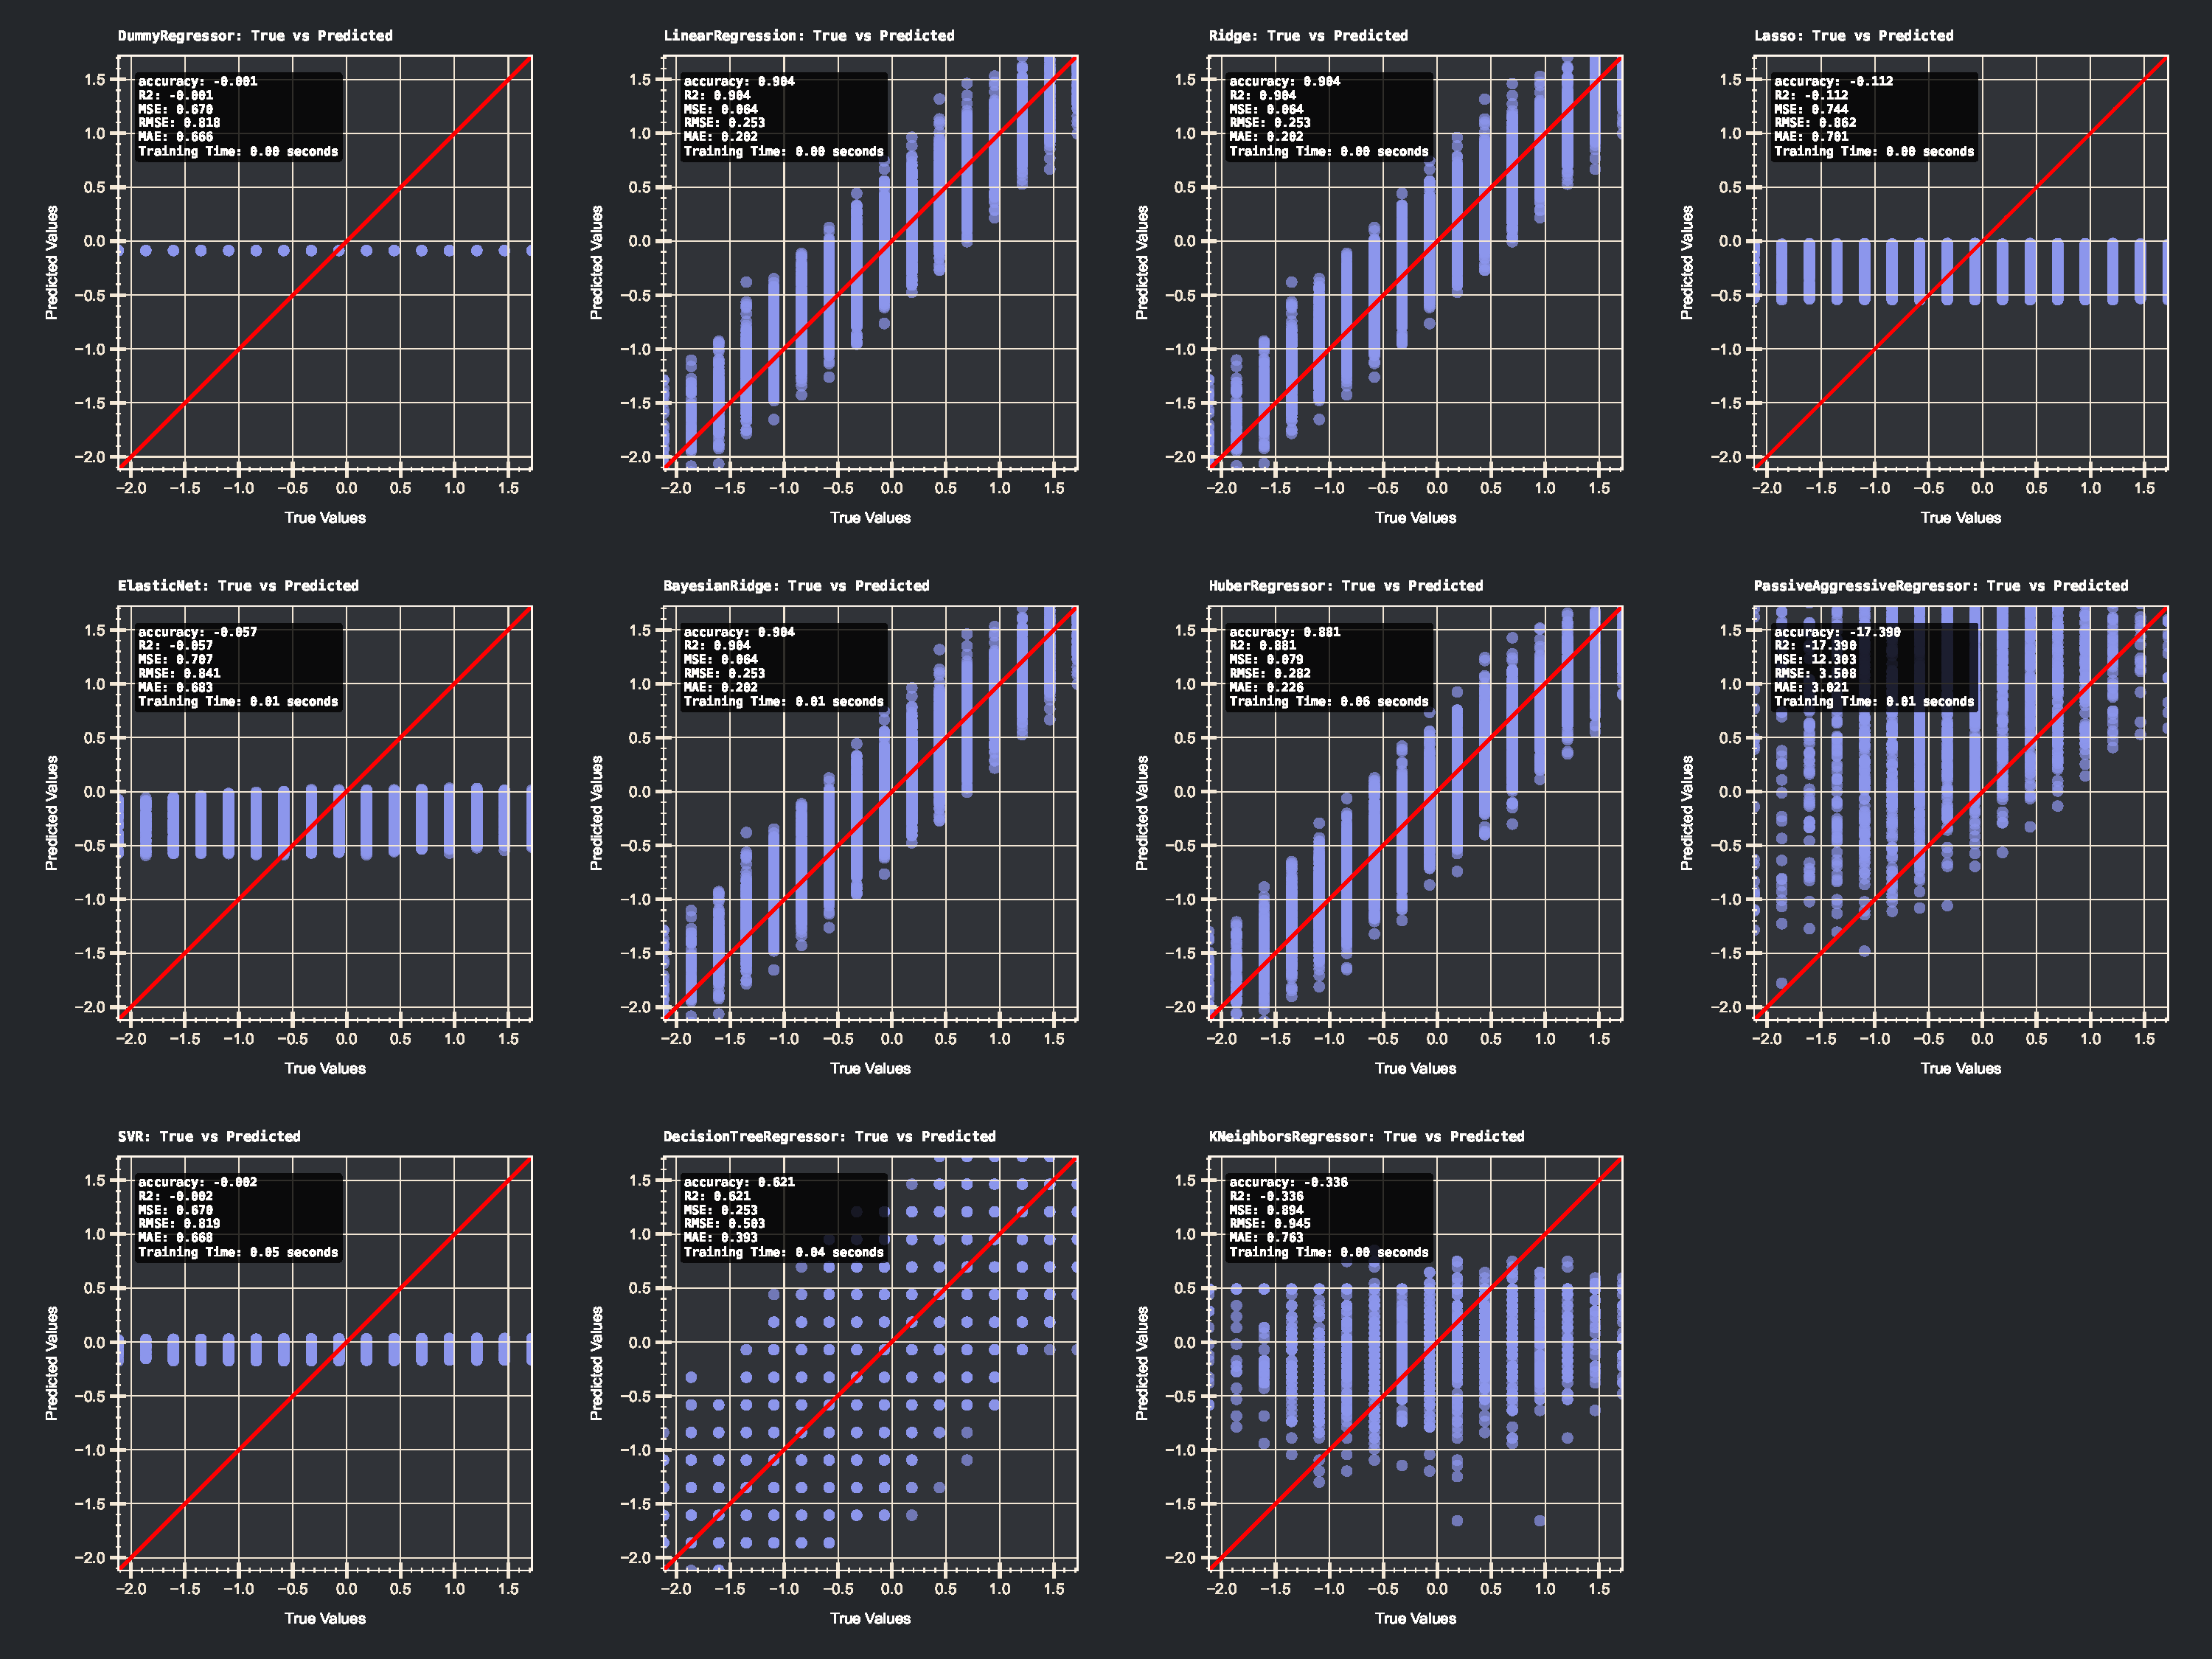
\includegraphics[width=6.5in]{../report/assets/base_models_results.pdf}    
    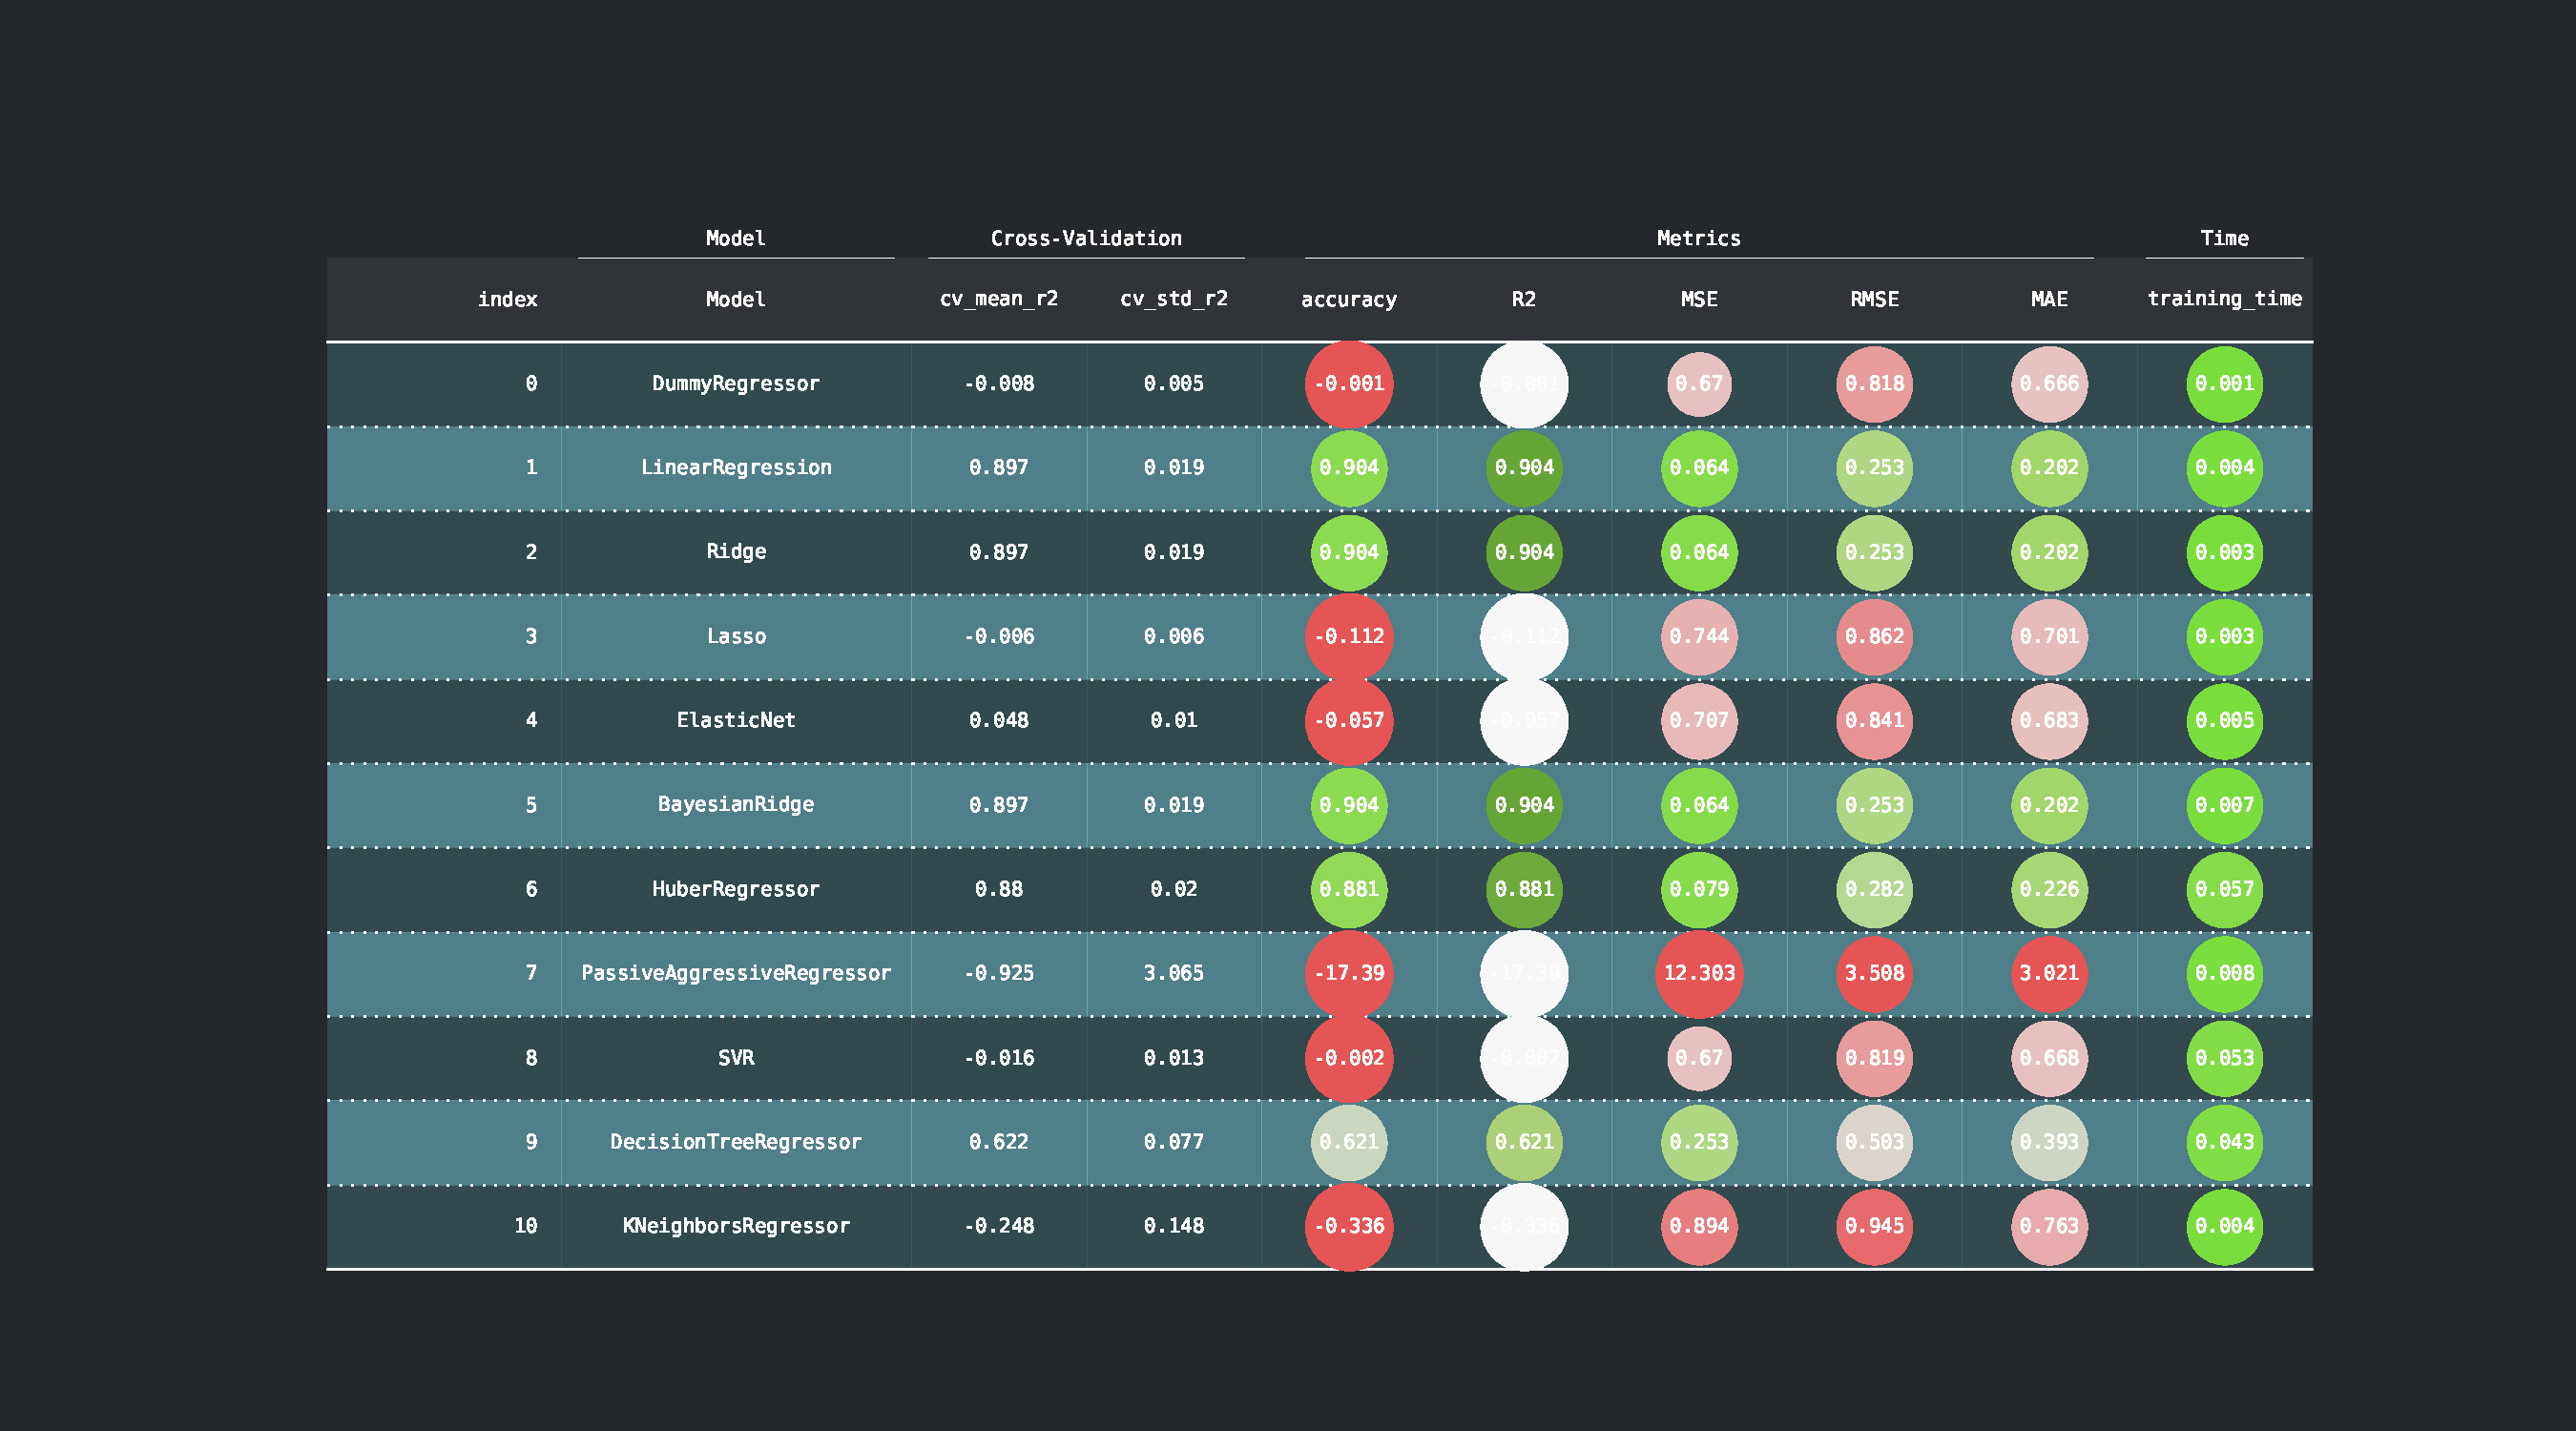
\includegraphics[width=6.5in]{../report/assets/base_models_results_table.pdf}    
\end{center}
I then tried some more advanced models such as RandomForestRegressor, BaggingRegressor, StackingReggressor.
Essentially pulling out all the ensemble methods I could find in the scikit-learn library.
\begin{center}
    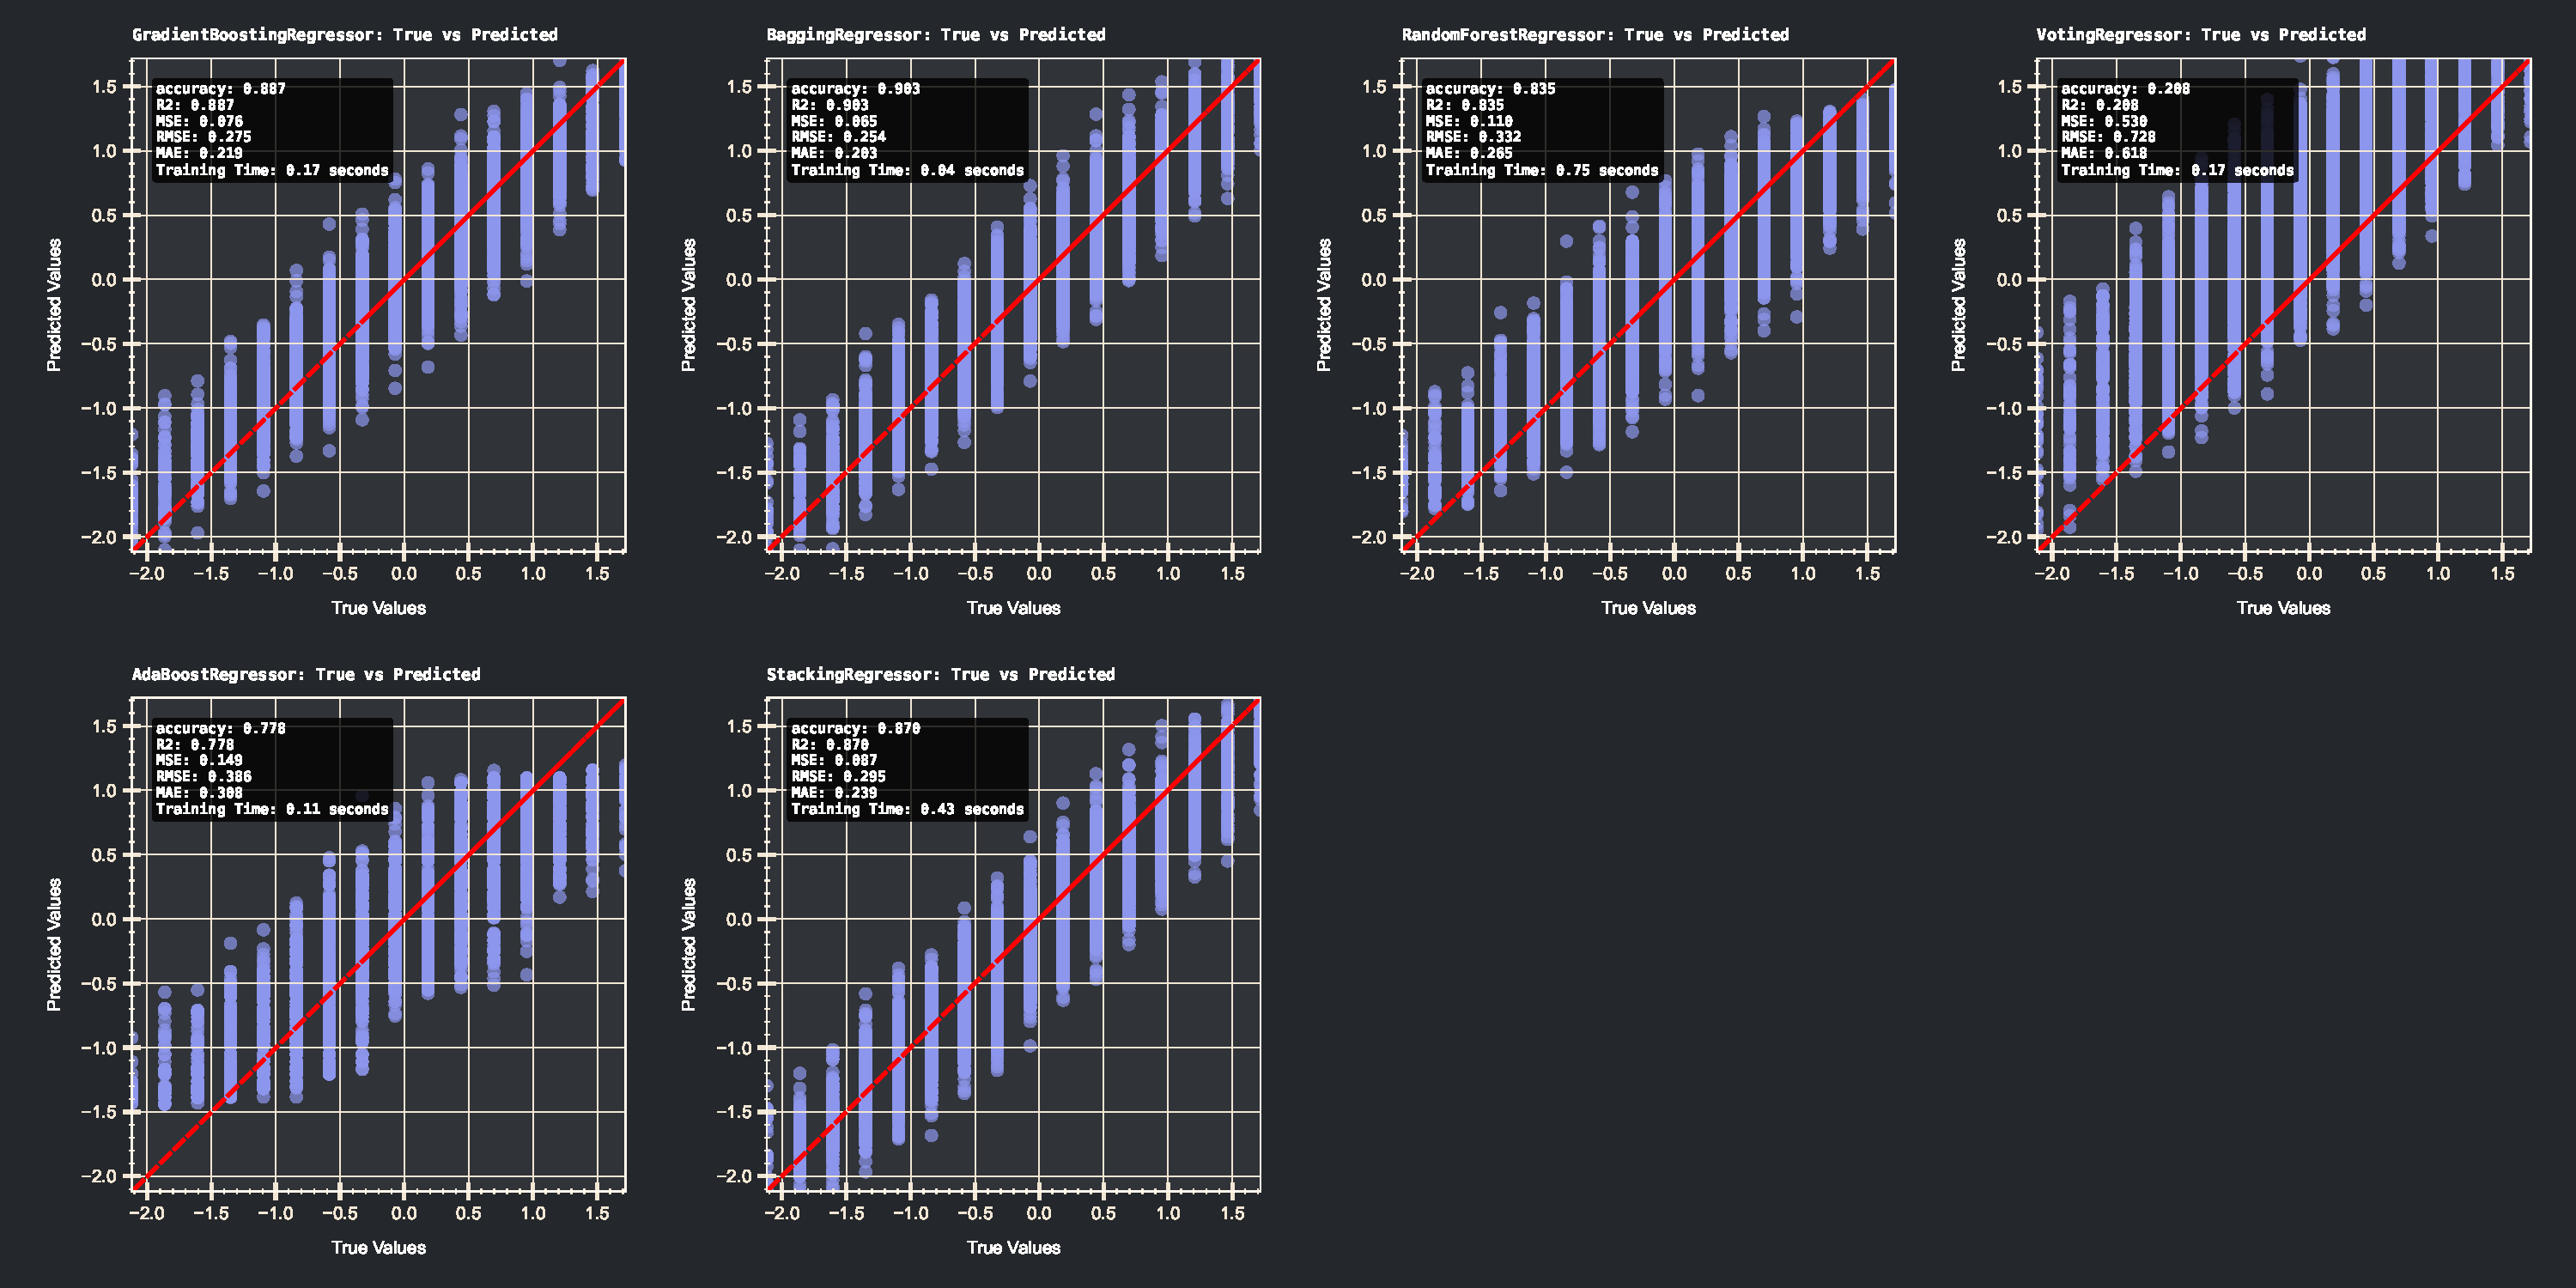
\includegraphics[width=6.5in]{../report/assets/ensemble_methods_results.pdf}    
    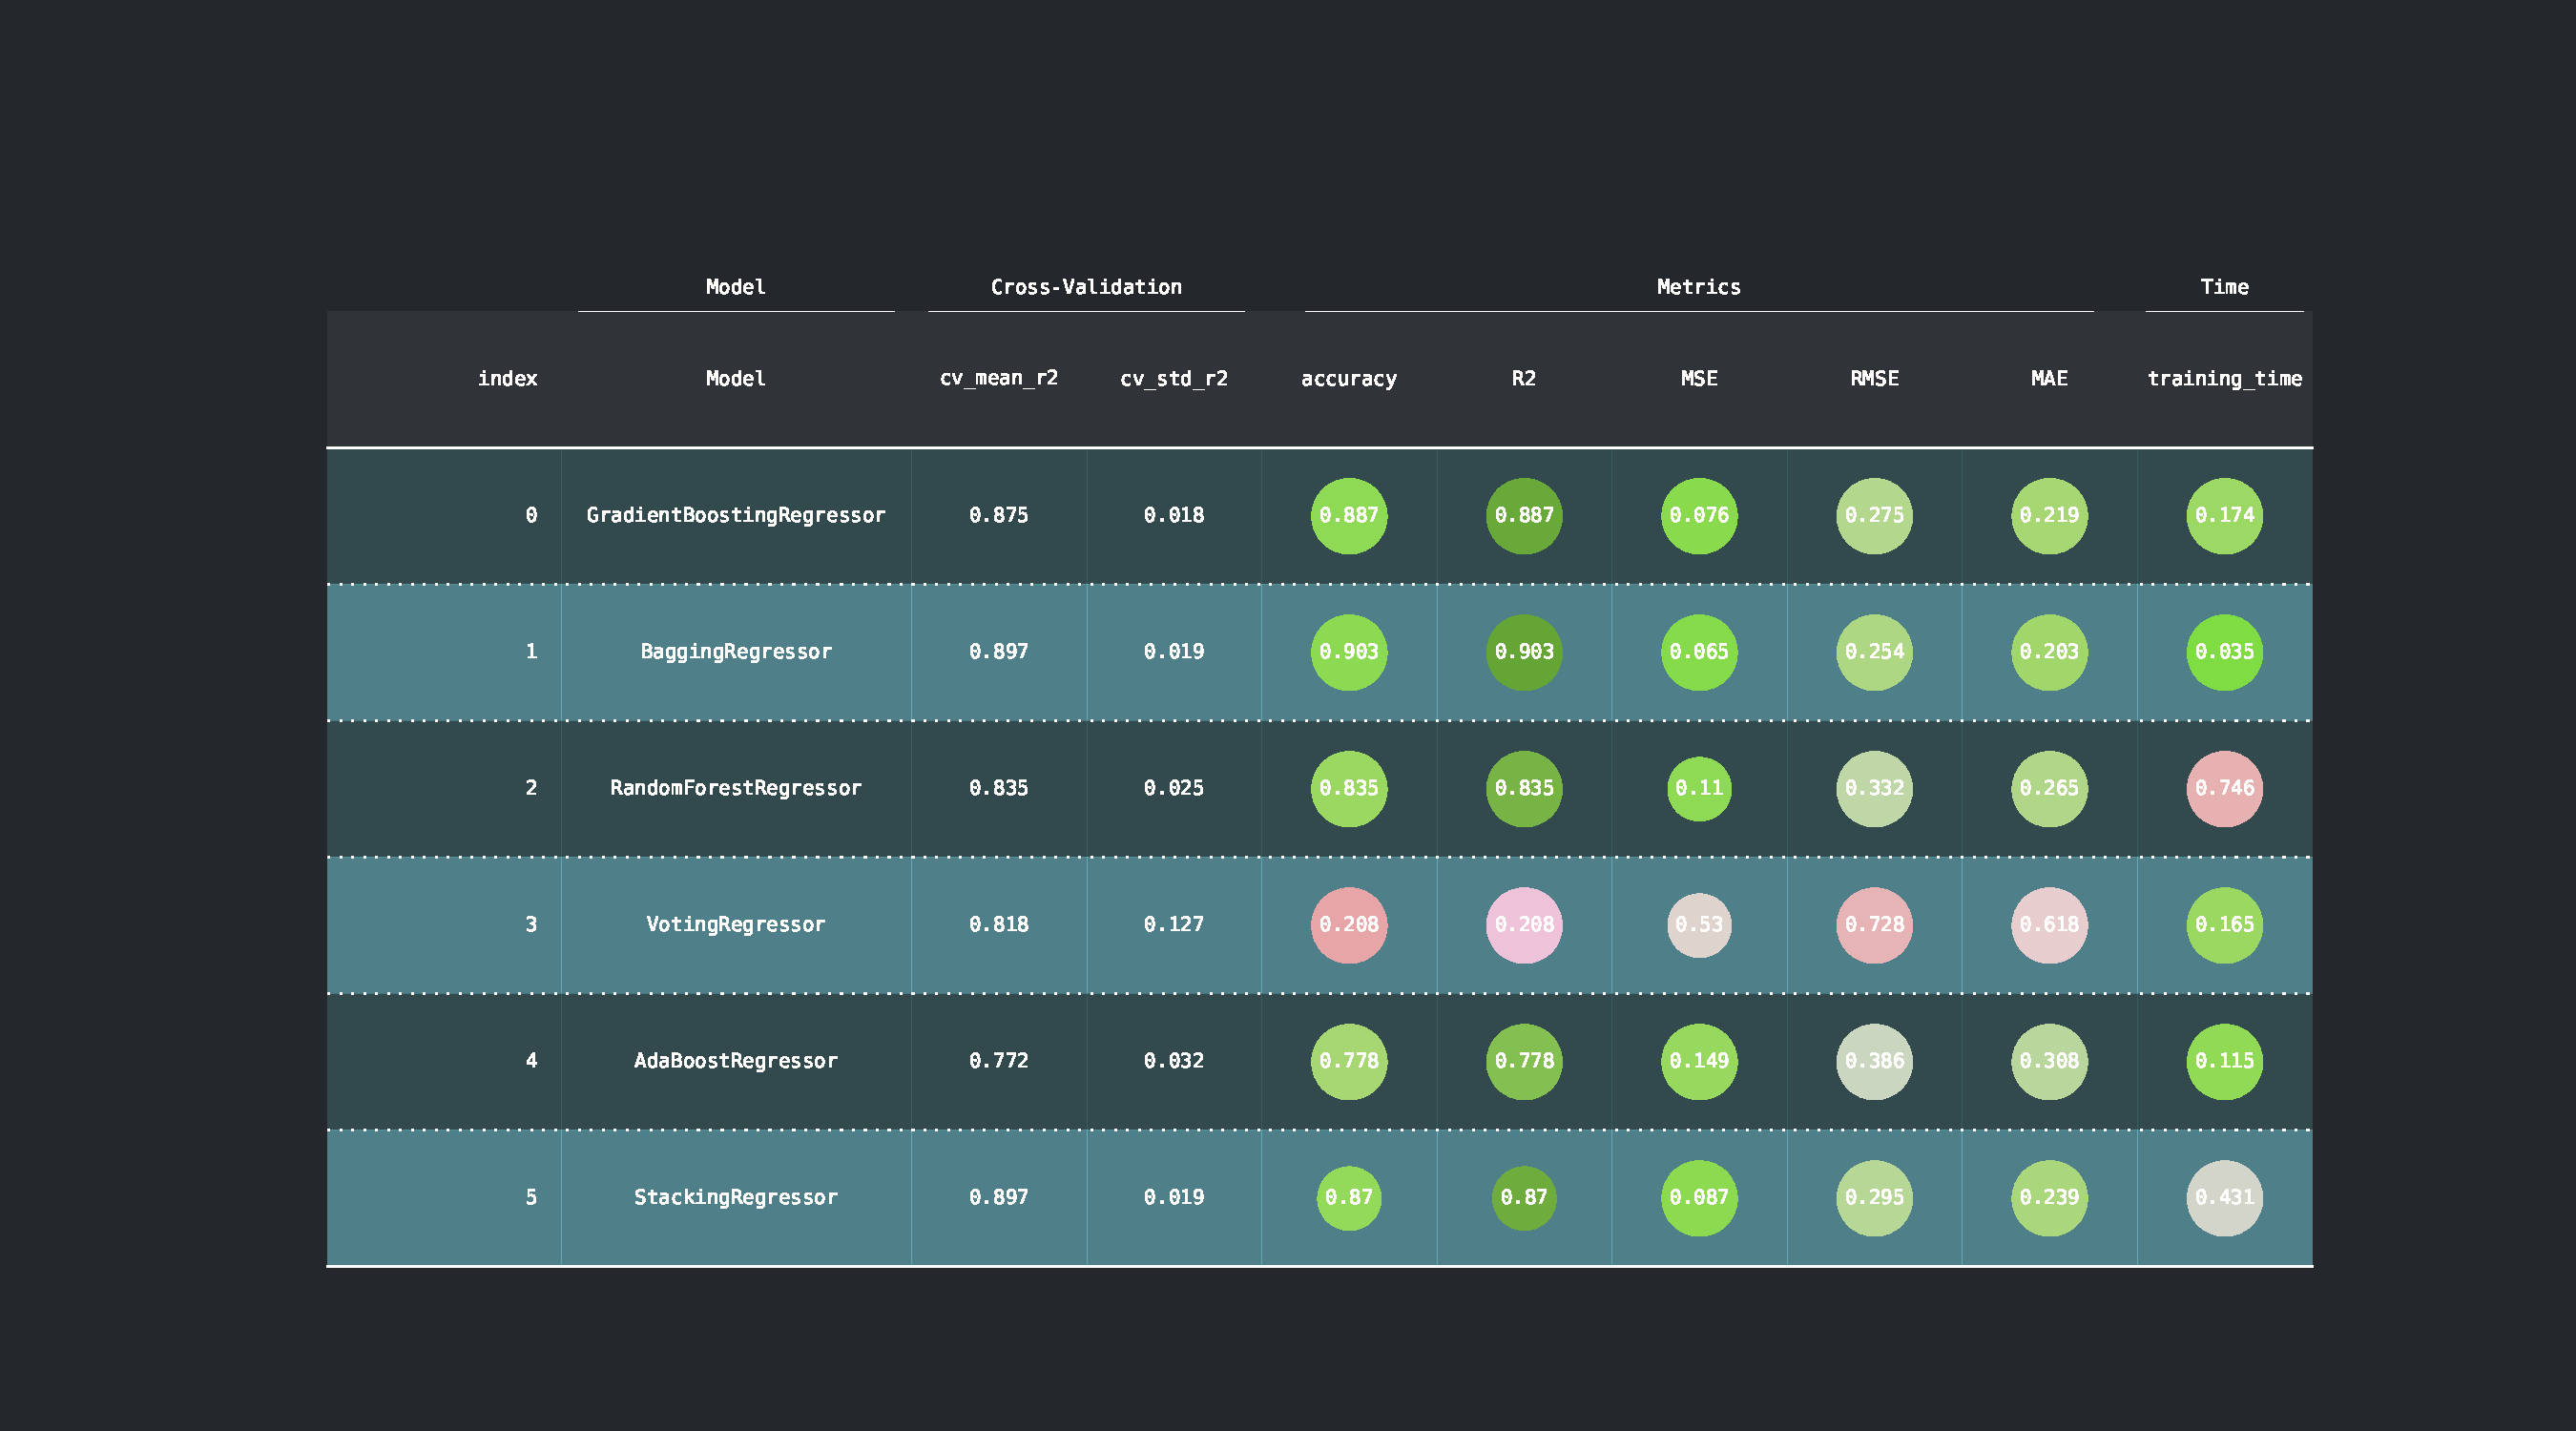
\includegraphics[width=6.5in]{../report/assets/ensemble_methods_results_table.pdf}    
\end{center}
These models performed better than the baseline models, but still not good enough to achieve the goal of a MSE close to 0 but i was already under a margin of 0.1.

Quick thing to note but very important is looking at the traing time with this size of a dataset, the training time of these models is very low, 
however i will always favor a simpler model over (LinearReggression) over any ensemble.
Why ? If you take a look at the CSV files,the training time of the LinearReggression model is significantly lower than the training time of the ensemble models.
In fact the training times are almost 100 times lower than the training time of the ensemble models.

However , we continue our search for the sake of education and to see if we can achieve a MSE close to 0.

\newpage
\subsection{Hyperparameter Tuning}
\subsubsection{Tuning}
The next step was to tune the hyperparameters of the best models to improve their performance.
I first used RandomSearchCV to search for the best hyperparameters for all the best models in our previous.
\begin{center}
    Version 1:
    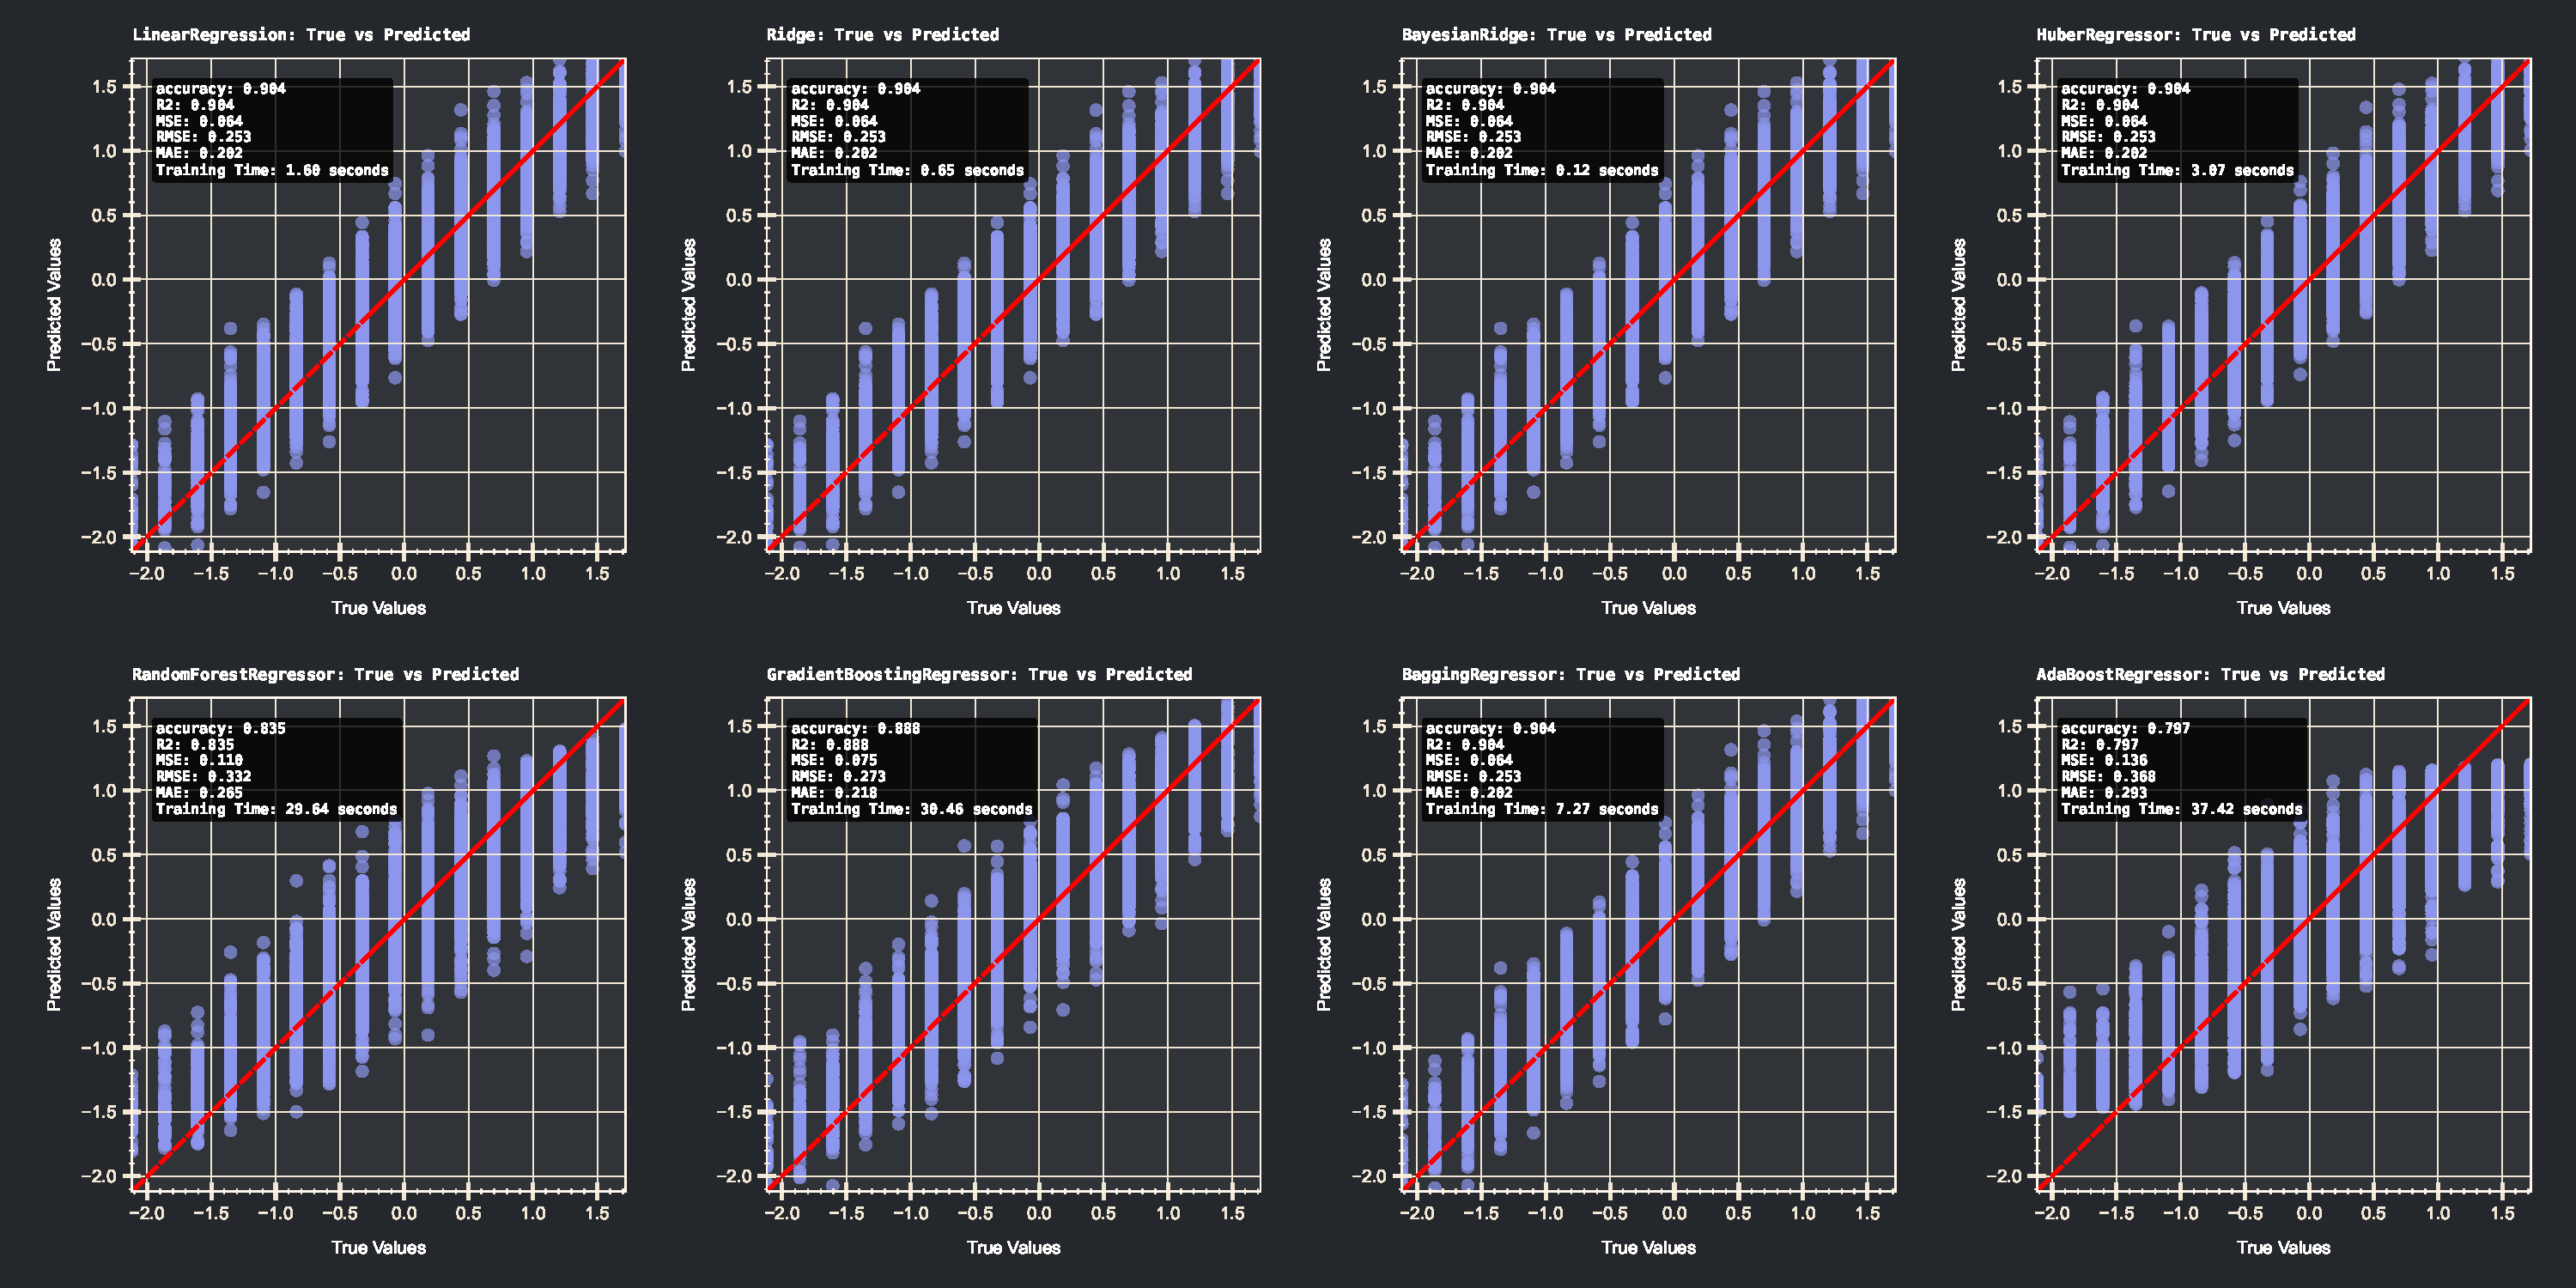
\includegraphics[width=6.5in]{../report/assets/ver1_best_models_result.pdf}    
    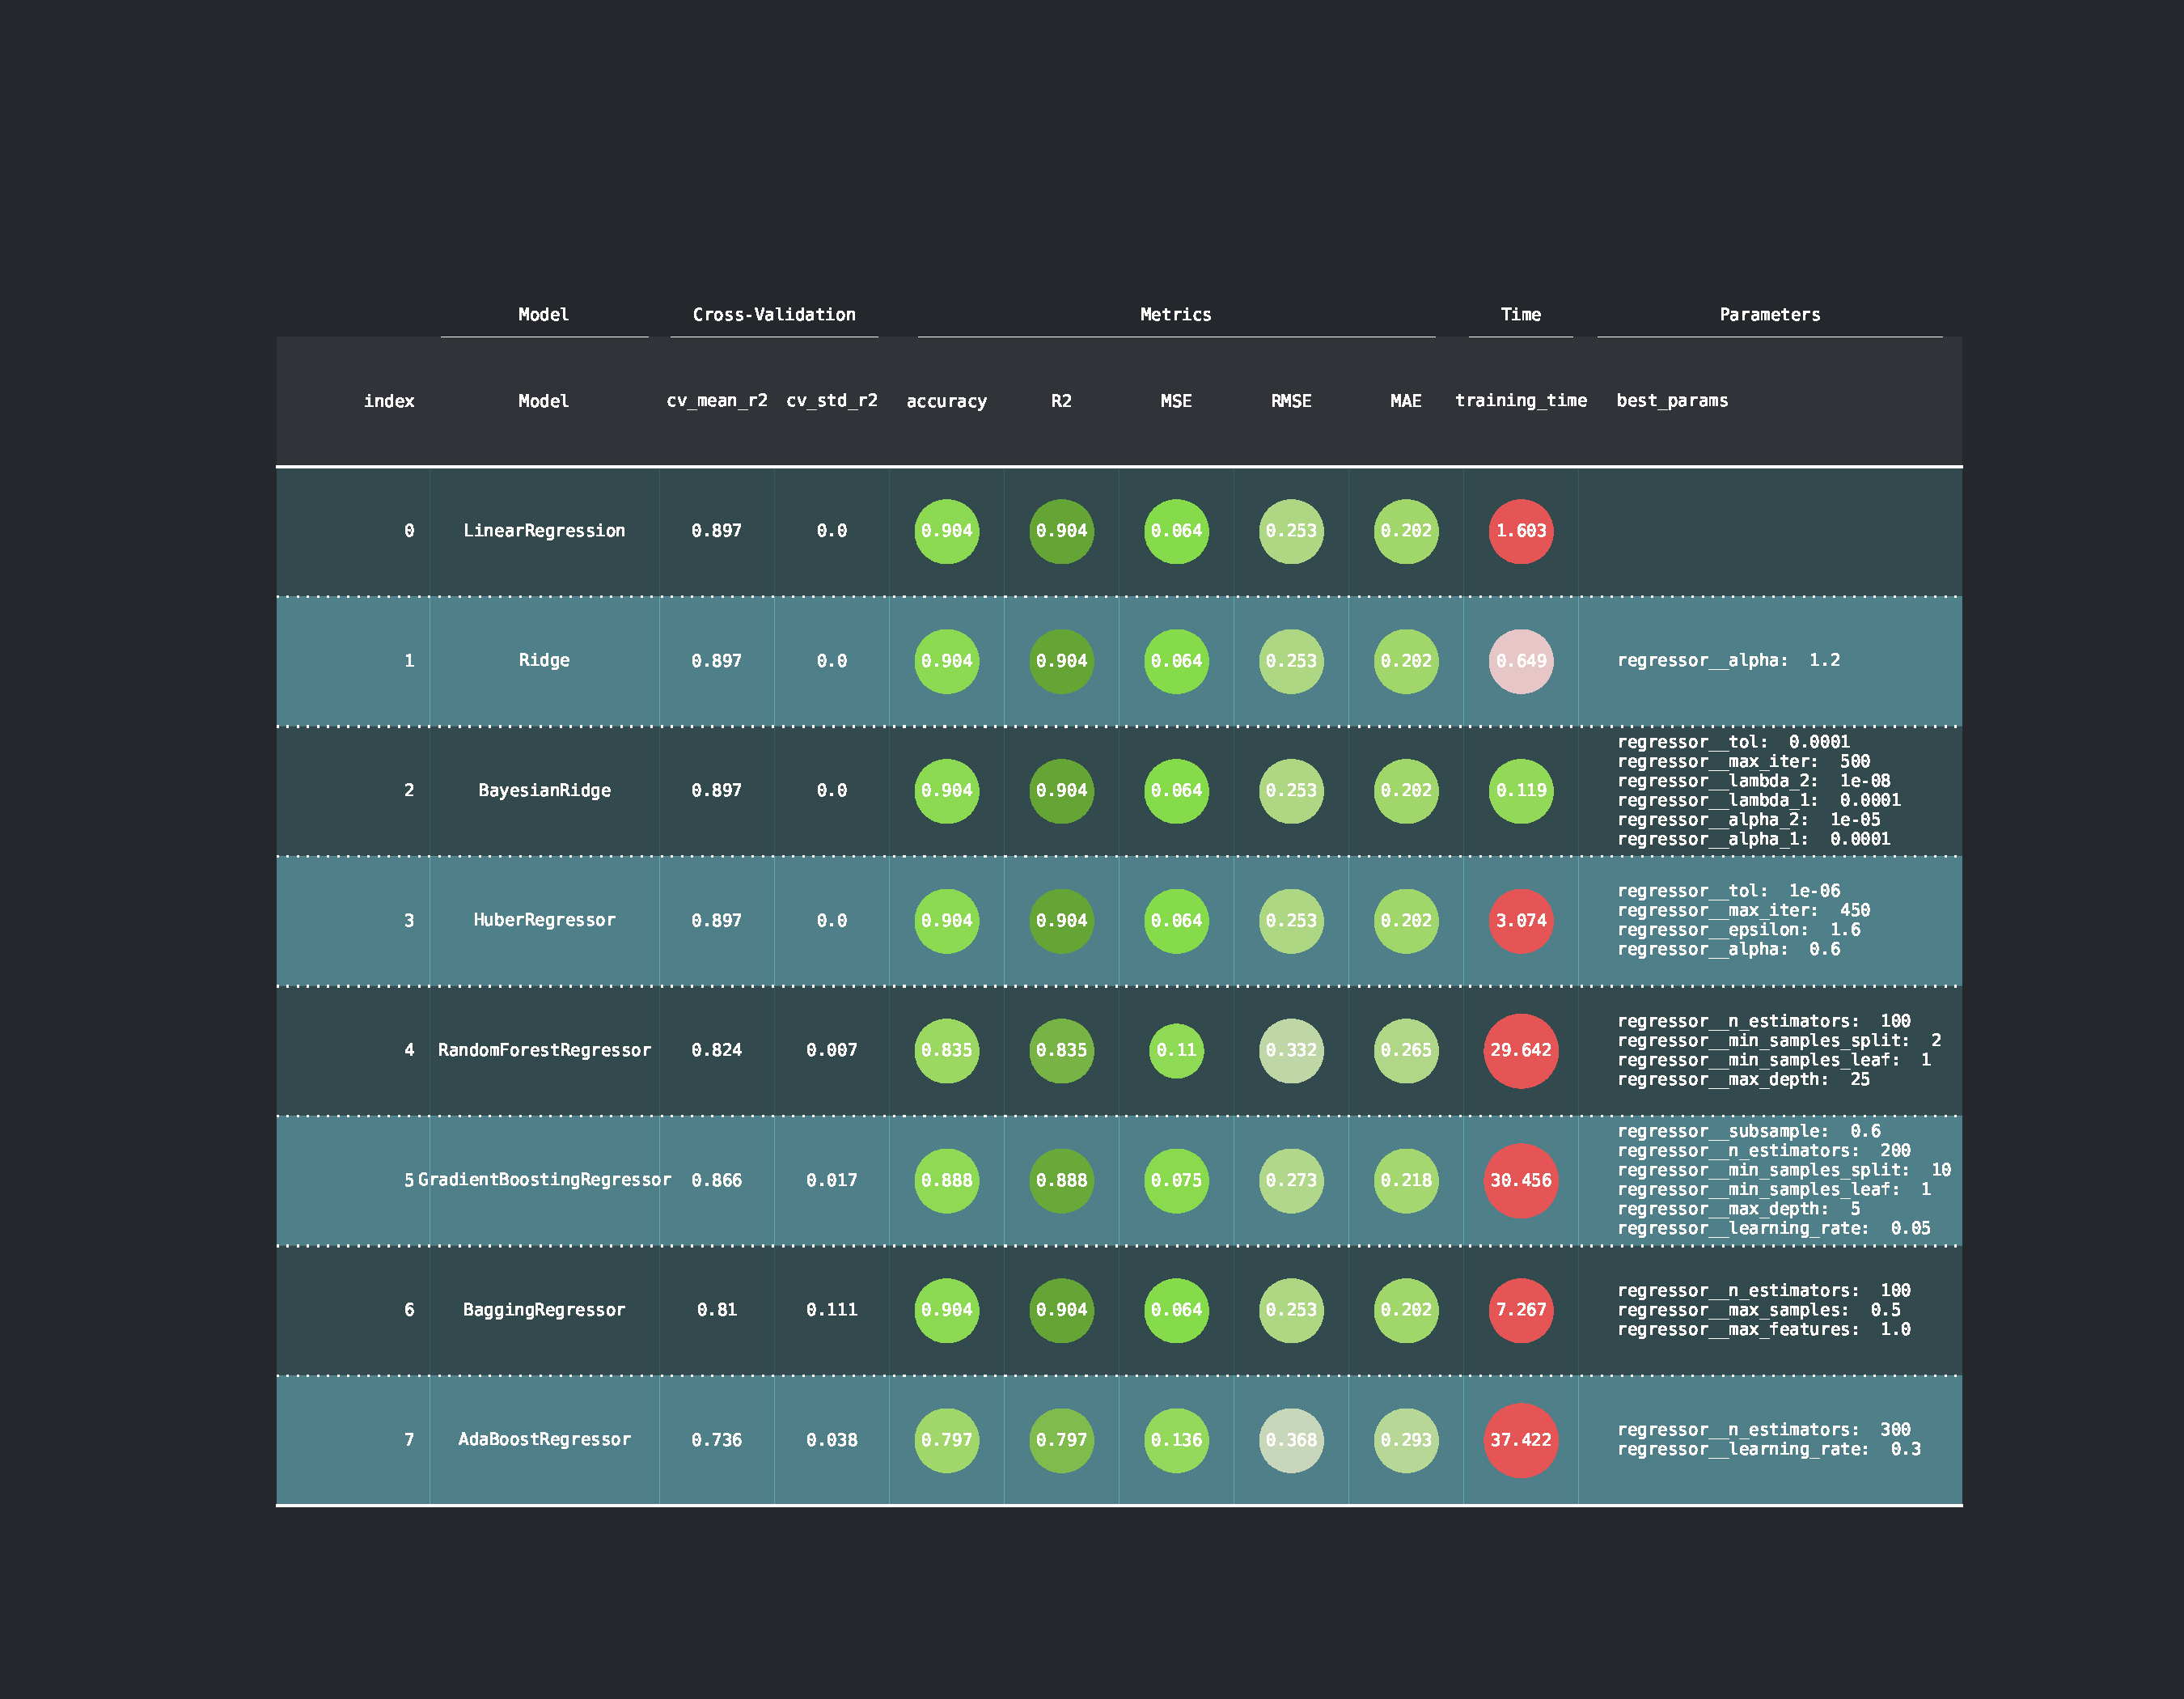
\includegraphics[width=6.5in]{../report/assets/ver1_best_models_result_table.pdf}
\end{center}
And then I used GridSearchCV to search for the best hyperparameters for the best model from the previous step and eliminating the ones that perform less good along the way.
repeating this process until I found the best hyperparameters for the best model.
\begin{center}
    Version 4:
    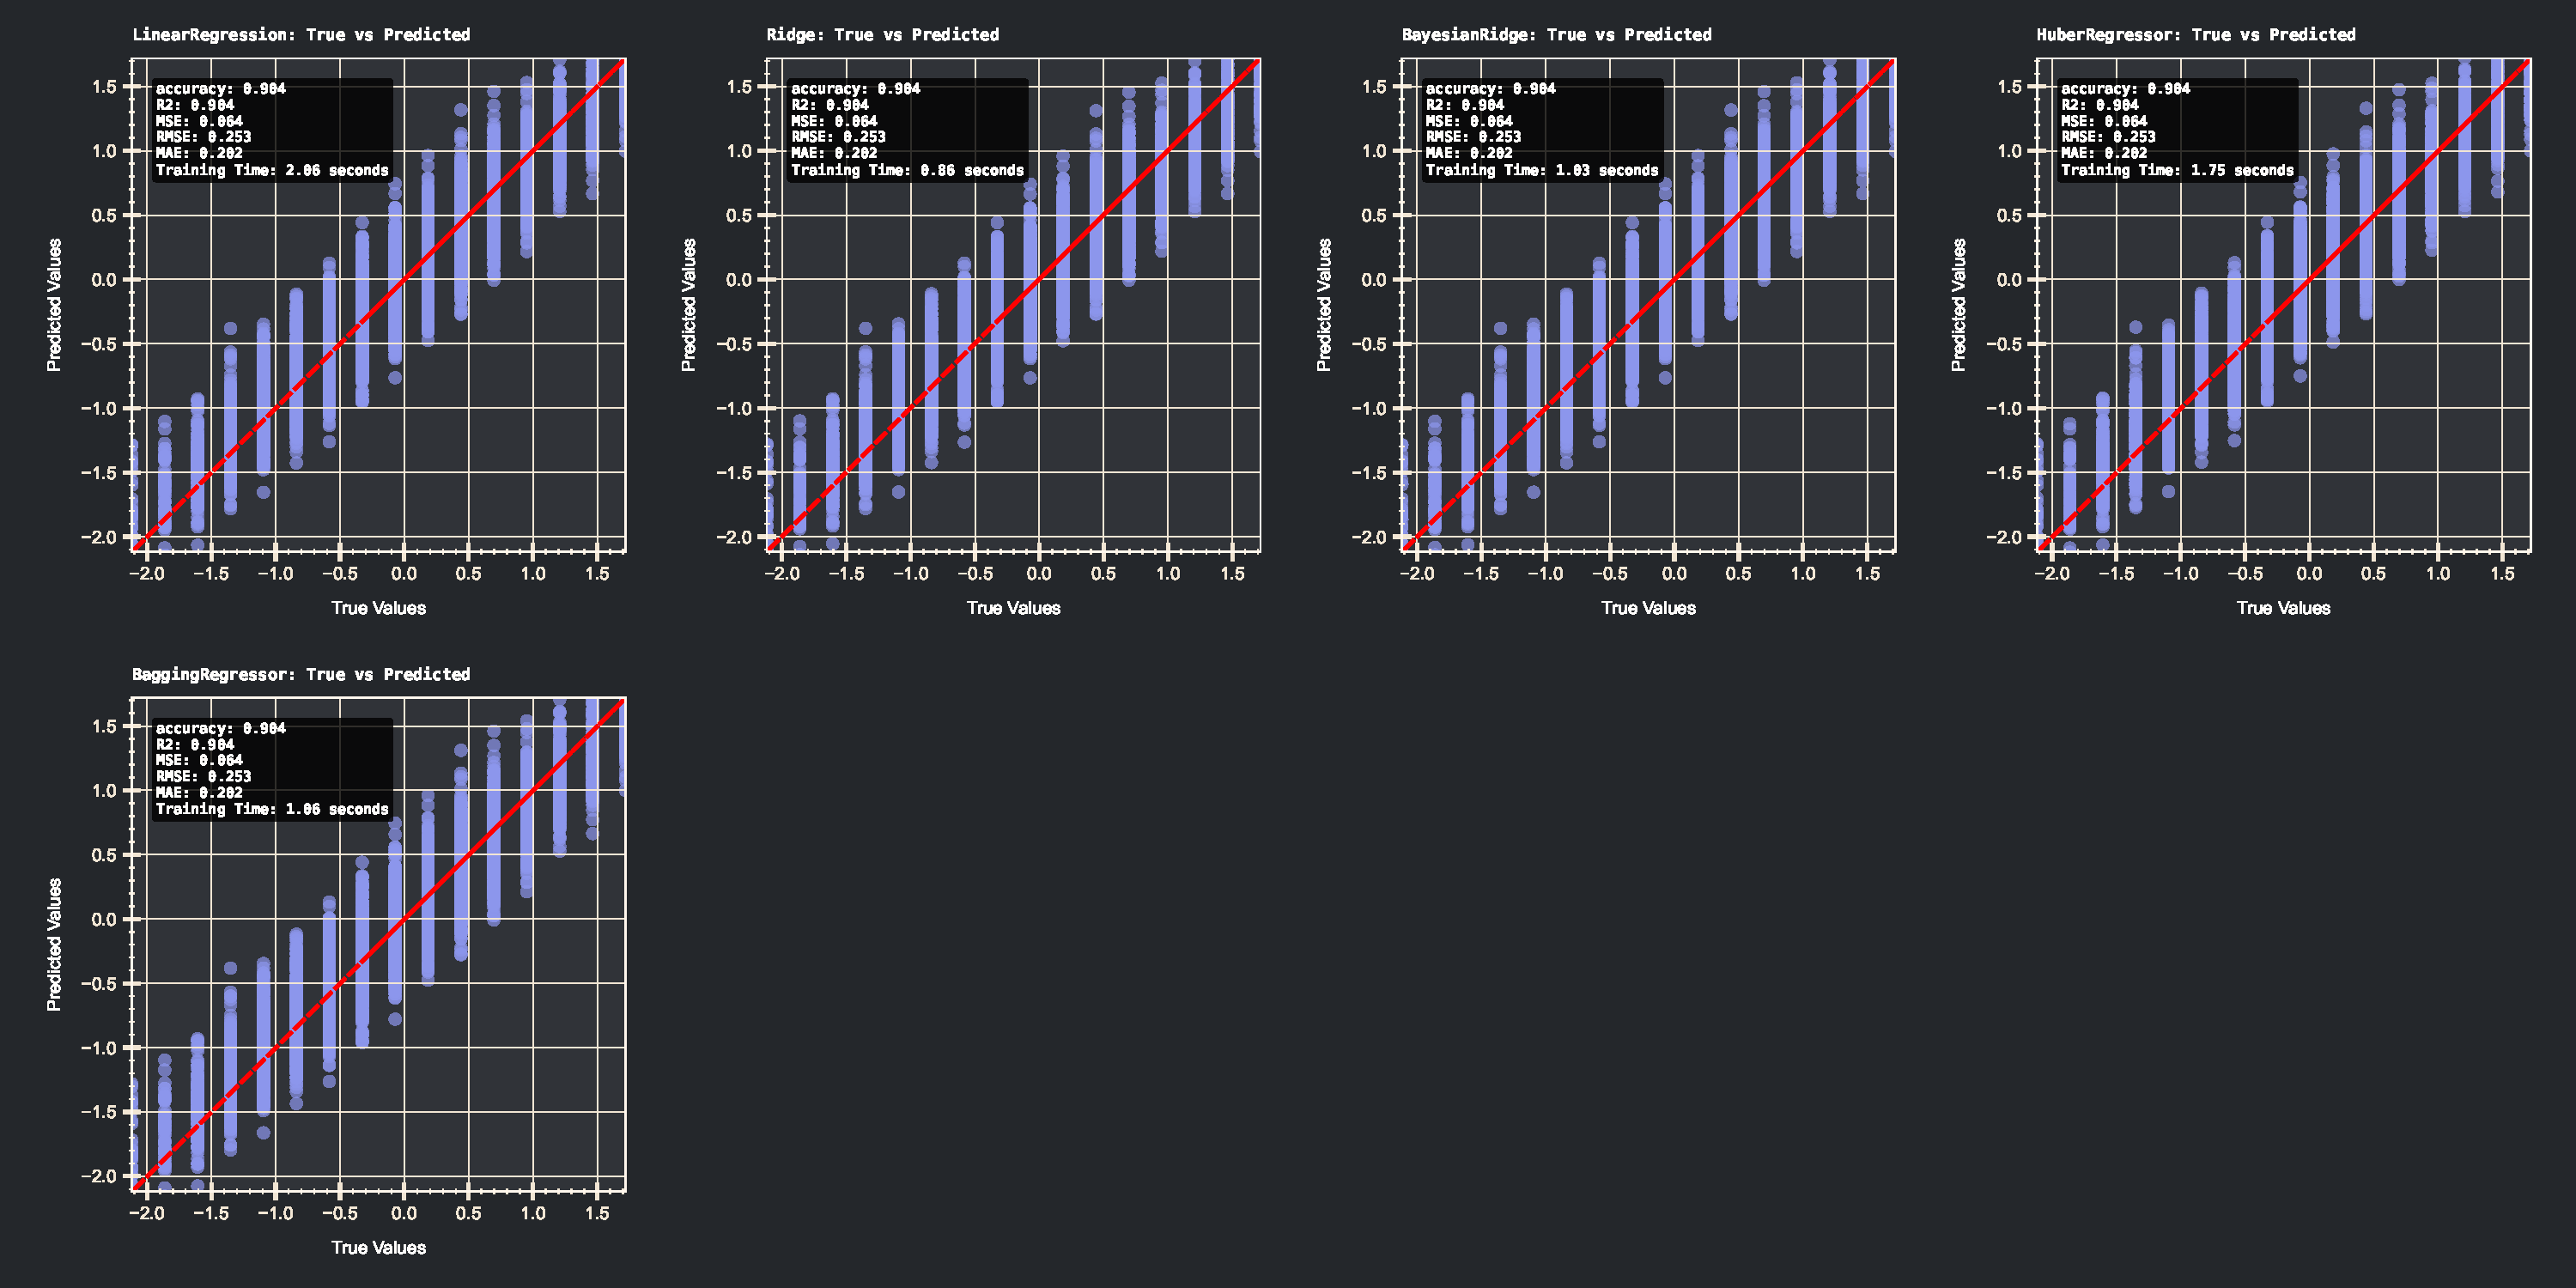
\includegraphics[width=6.5in]{../report/assets/ver4_best_models_result.pdf}    
    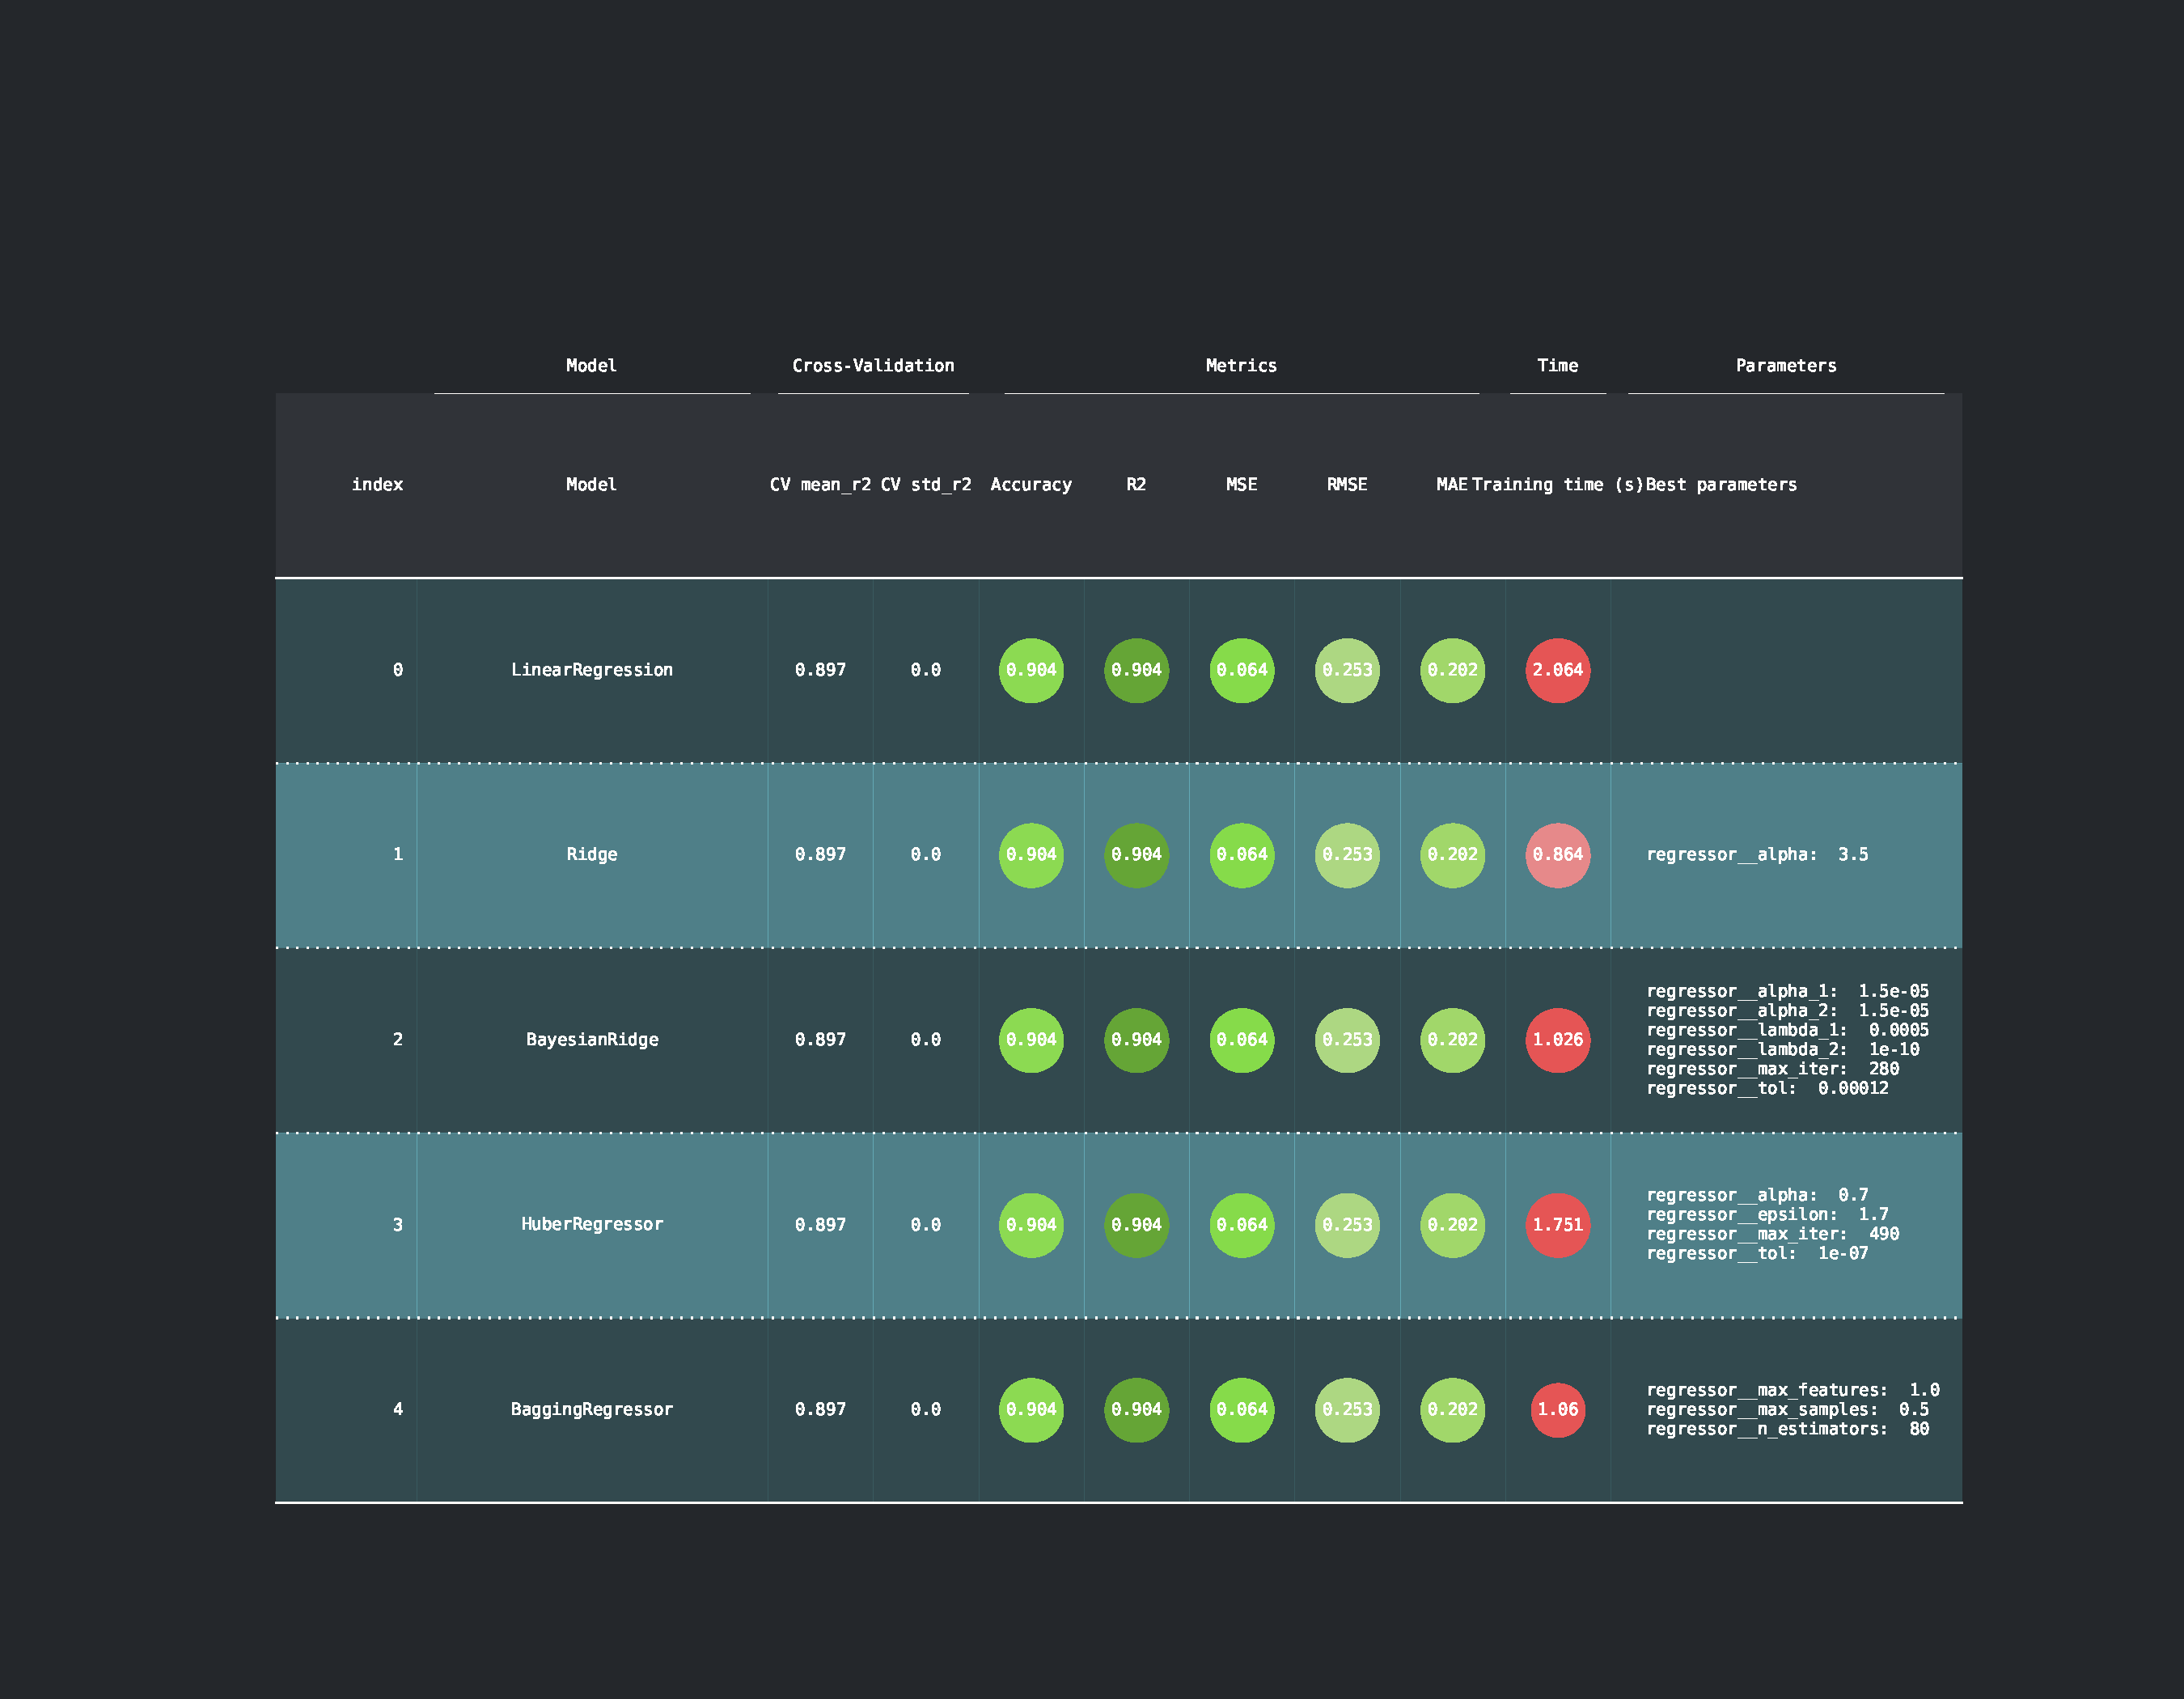
\includegraphics[width=6.5in]{../report/assets/ver4_best_models_result_table.pdf}
\end{center}
By the time i reached version 7 i had already achieved a MSE of 0.1 and i was not able to improve the performance of the models any further. 
Using the best models and their best hyperparameters, i was able to achieve a MSE of below 0.1 on the test set.
Then loading the best model and using ensemble methods again it will yield the same results to a lack of diversity in the models.
\begin{center}
    Ensemble 1:
    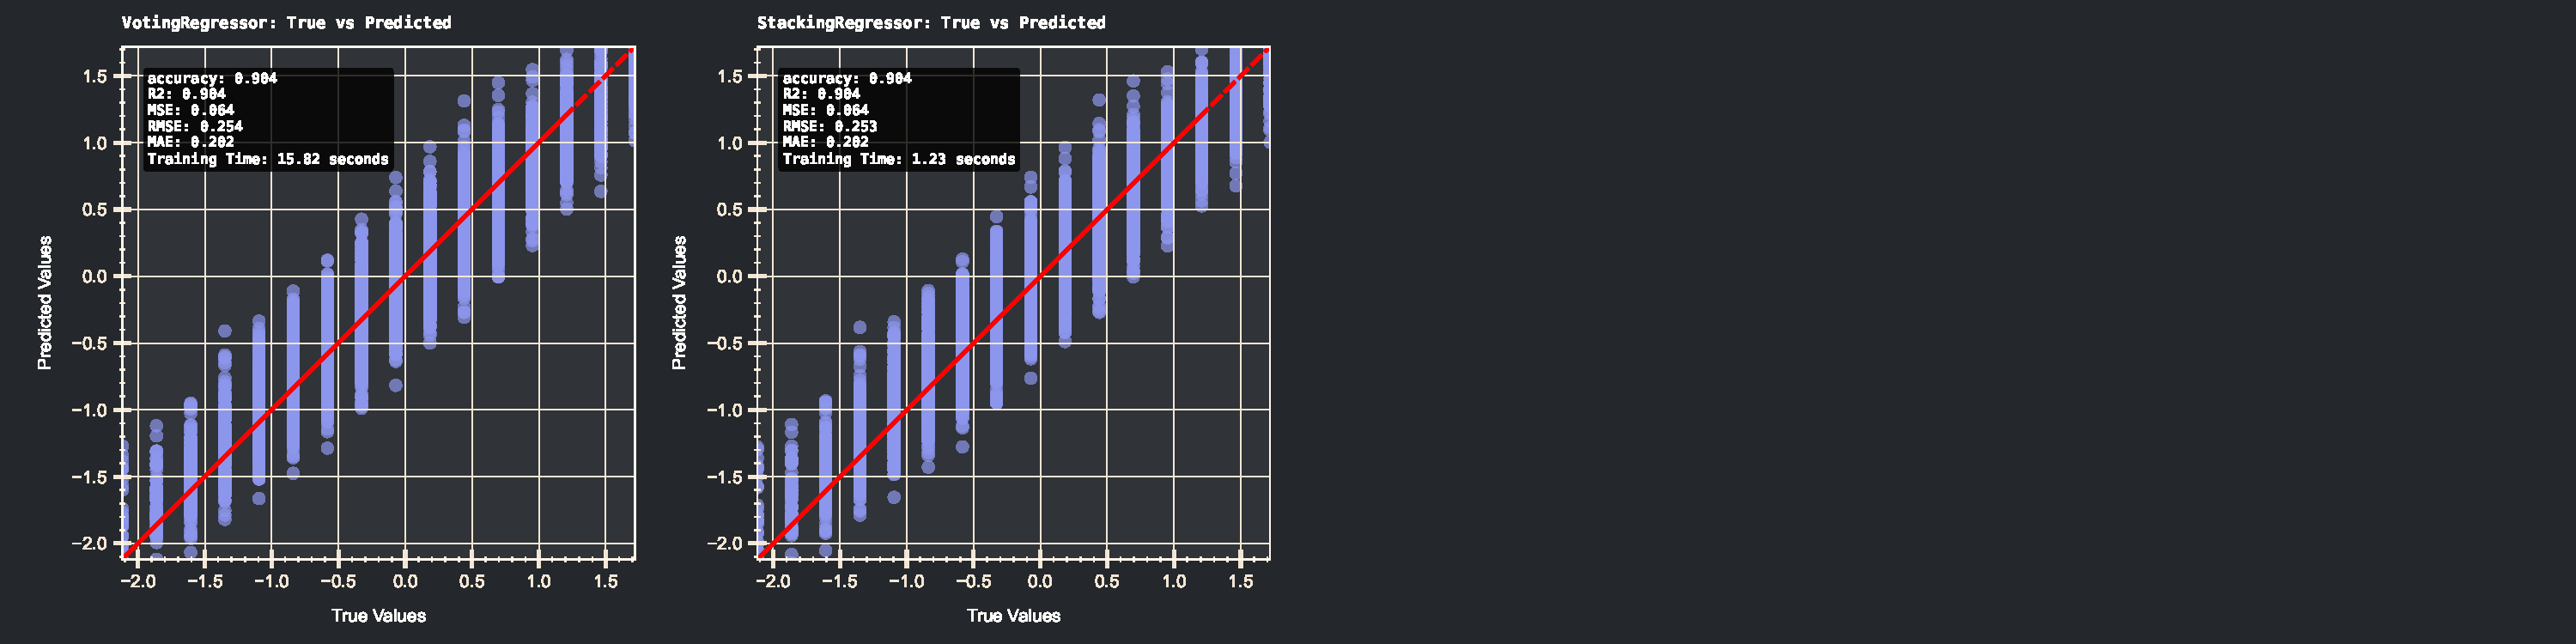
\includegraphics[width=6.5in]{../report/assets/ensemble_1_best_models_result.pdf}    
    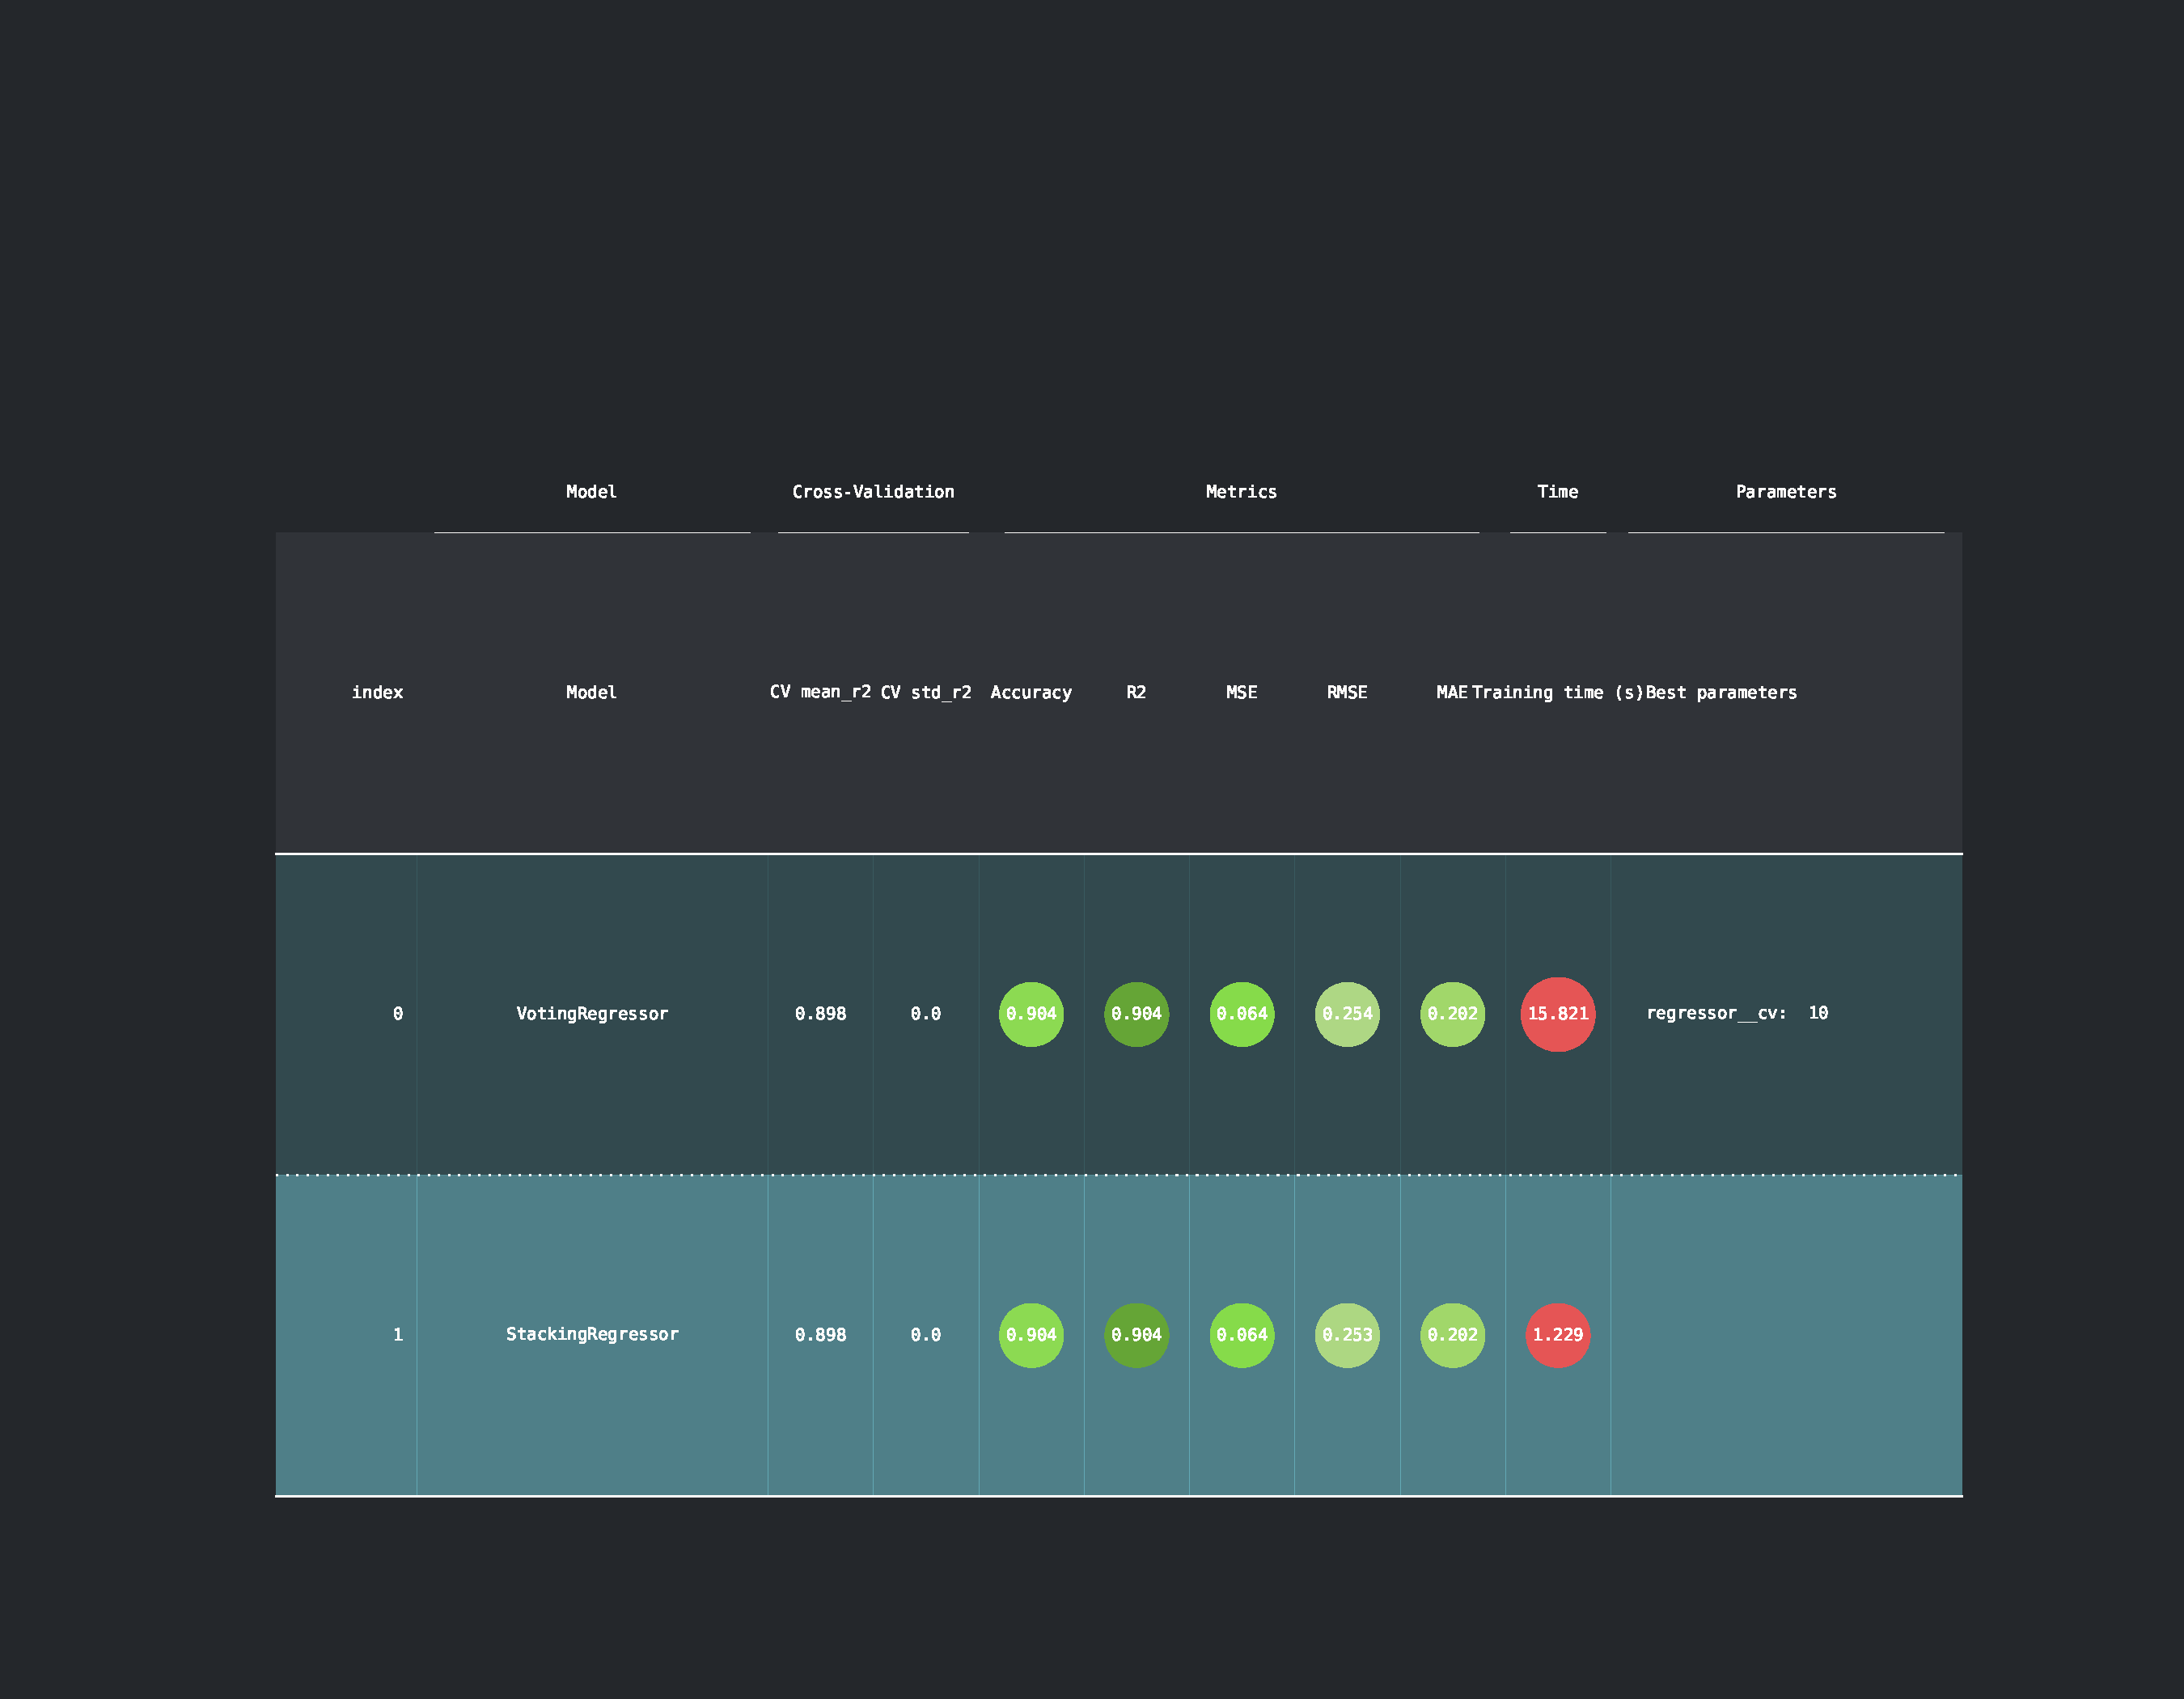
\includegraphics[width=6.5in]{../report/assets/ensemble_1_best_models_result_table.pdf}
\end{center}

\subsubsection{Final Model}
The final best models were:
\begin{enumerate}
    \item \textbf{Linear Regression} with a MSE of 0.064 on the test set
    \item \textbf{Ridge} with a MSE of 0.064 on the test set
    \item \textbf{Bayesian Ridge} with a MSE of 0.064 on the test set
    \item \textbf{BaggingRegressor} with a MSE of 0.064 on the test set
    \item \textbf{HuberRegressor} with a MSE of 0.064 on the test set
    \item \textbf{VotingRegressor} with a MSE of 0.064 on the test set
    \item \textbf{StackingRegressor} with a MSE of 0.064 on the test set and with as final estimator a \textbf{Linear Regression} model.
\end{enumerate}
I did try to remove the features that i created earlier to see if it would improve the performance of the model, but it did not.  
In fact the performance of the model was worse.

\begin{center}
    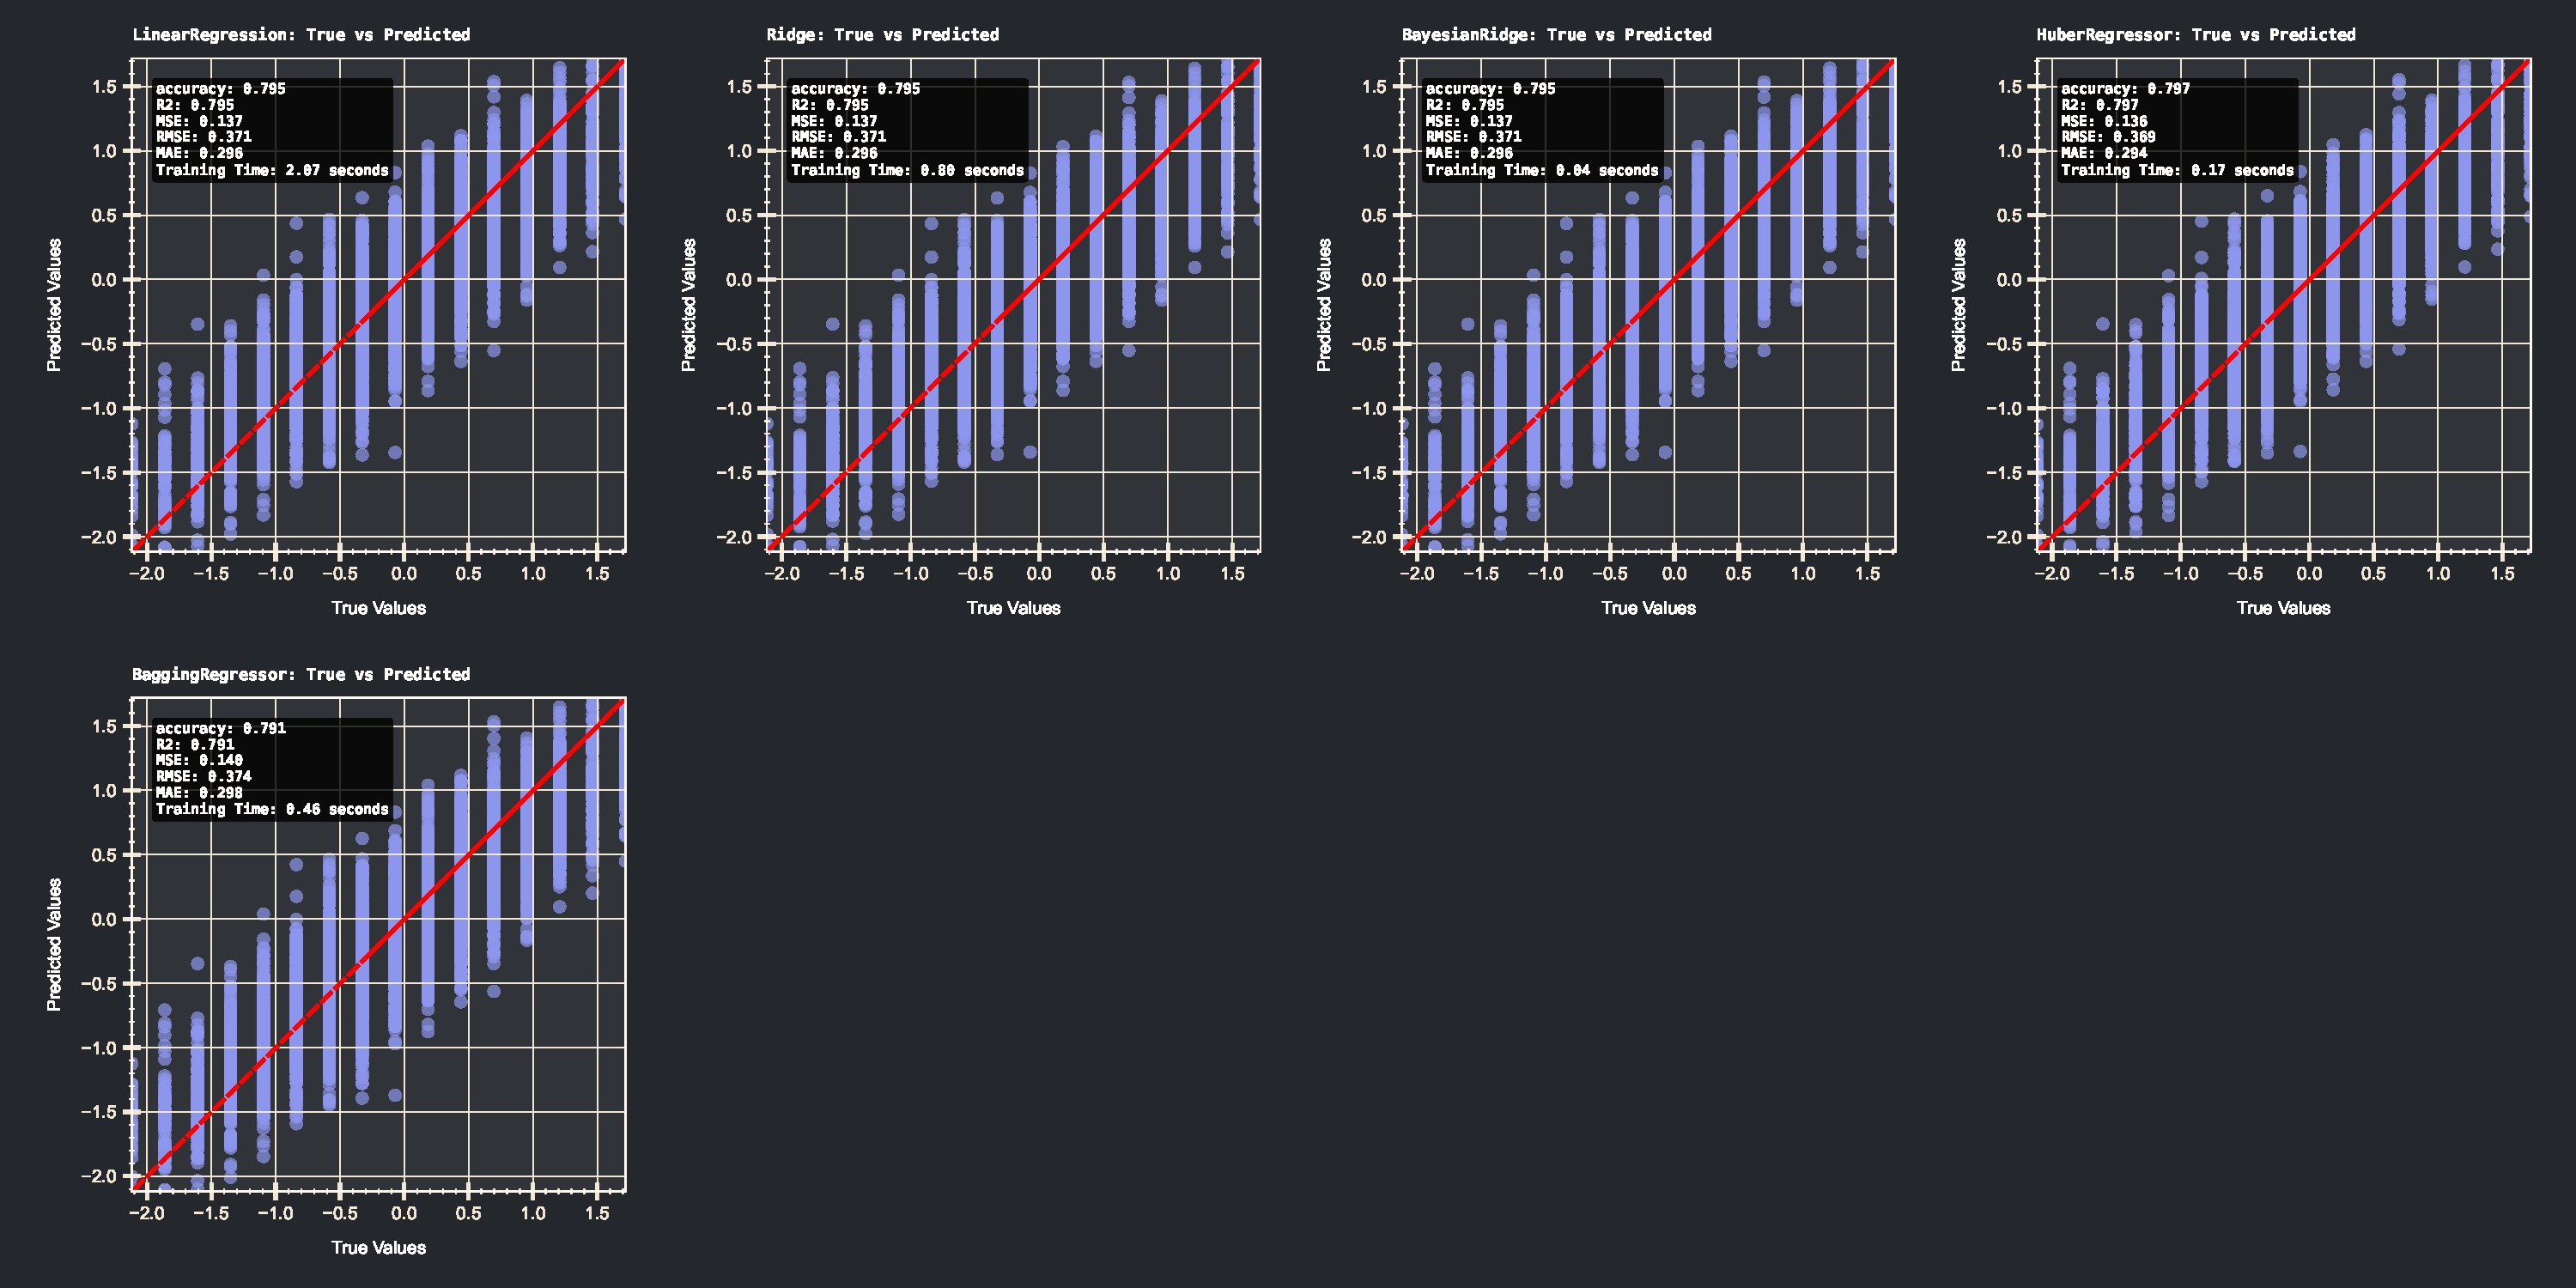
\includegraphics[width=6.5in]{../report/assets/remove_features_best_models_result.pdf}    
    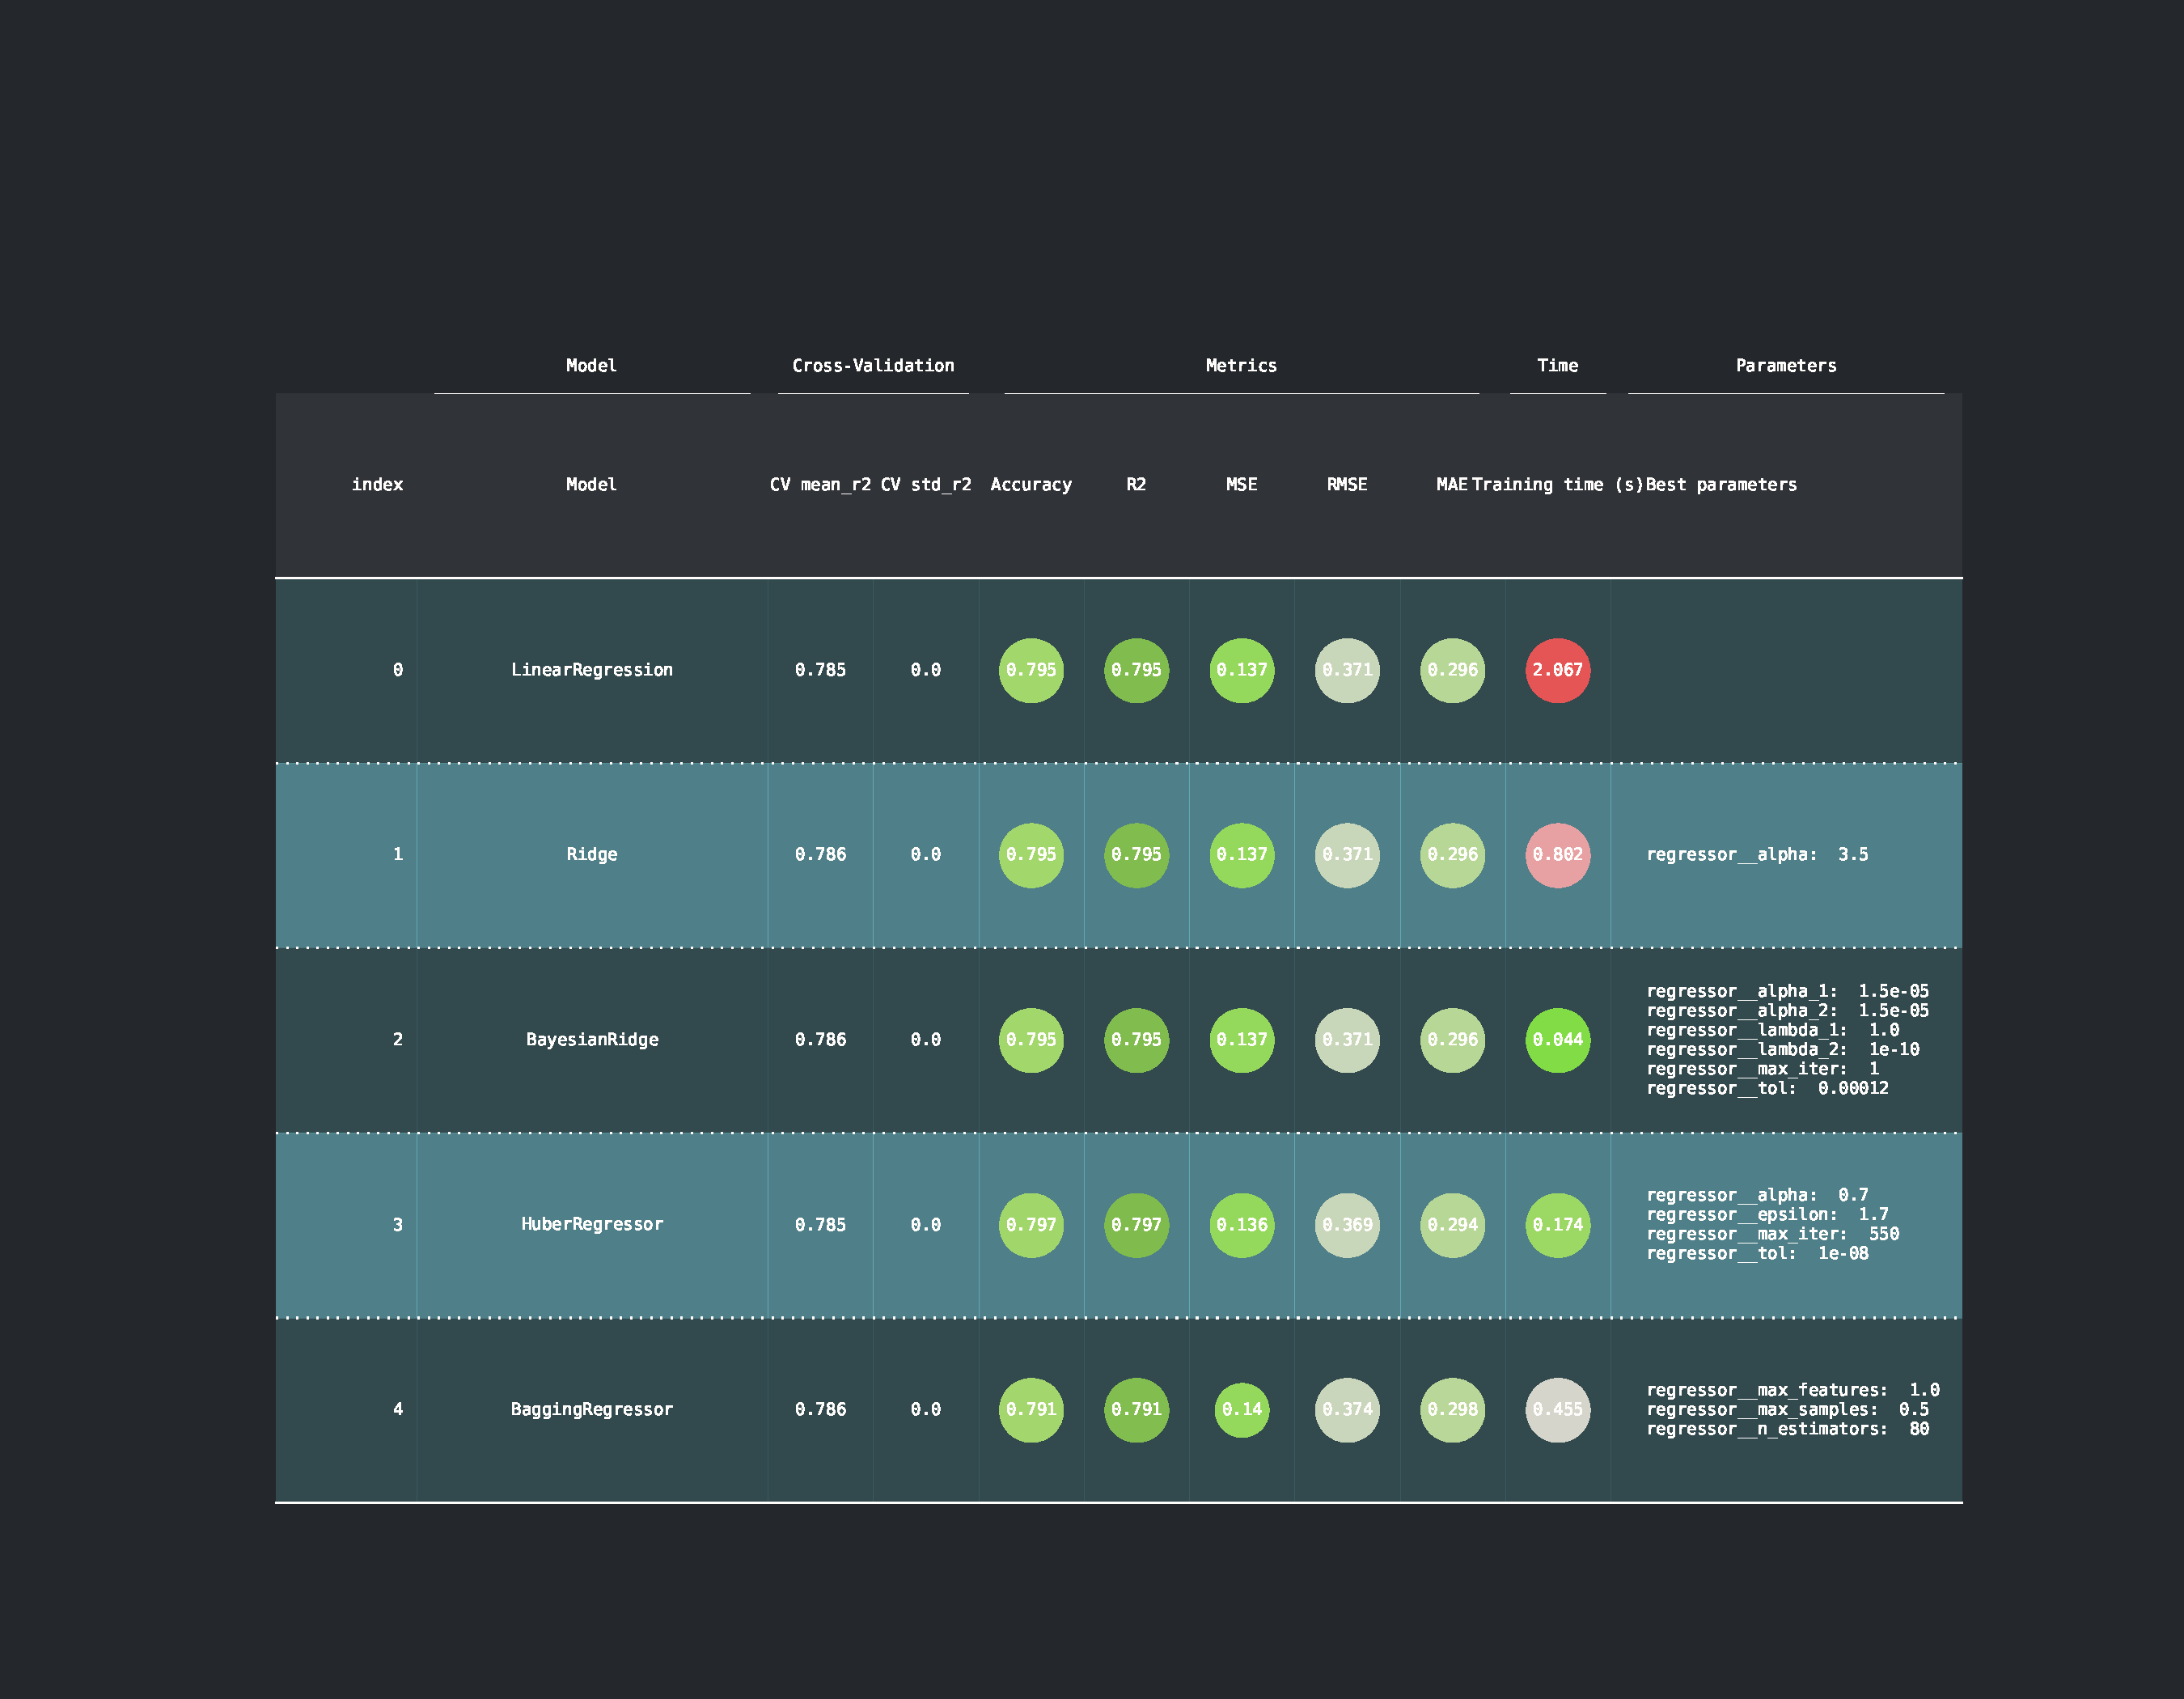
\includegraphics[width=6.5in]{../report/assets/remove_features_best_models_result_table.pdf}
\end{center}

I could also have tried to use more advanced models such as XGBoost, LightGBM, CatBoost, etc... but i did not have the time to do so.
A other that i could have done is to test different combination of features to see if it would improve the performance of the model.

\newpage
\subsection{Neural Networks}
However i did try to use a neural network to see if it would improve the performance of the model.
I first tried to use scikit-learn's MLPRegressor, which is a simple feedforward neural network.  
\lstinputlisting[style=independentpython,language=python,linerange={92-102}]{../chap_5_awakening_the_neural_mind/part_1_building_the_mind.py} 
\begin{center}
    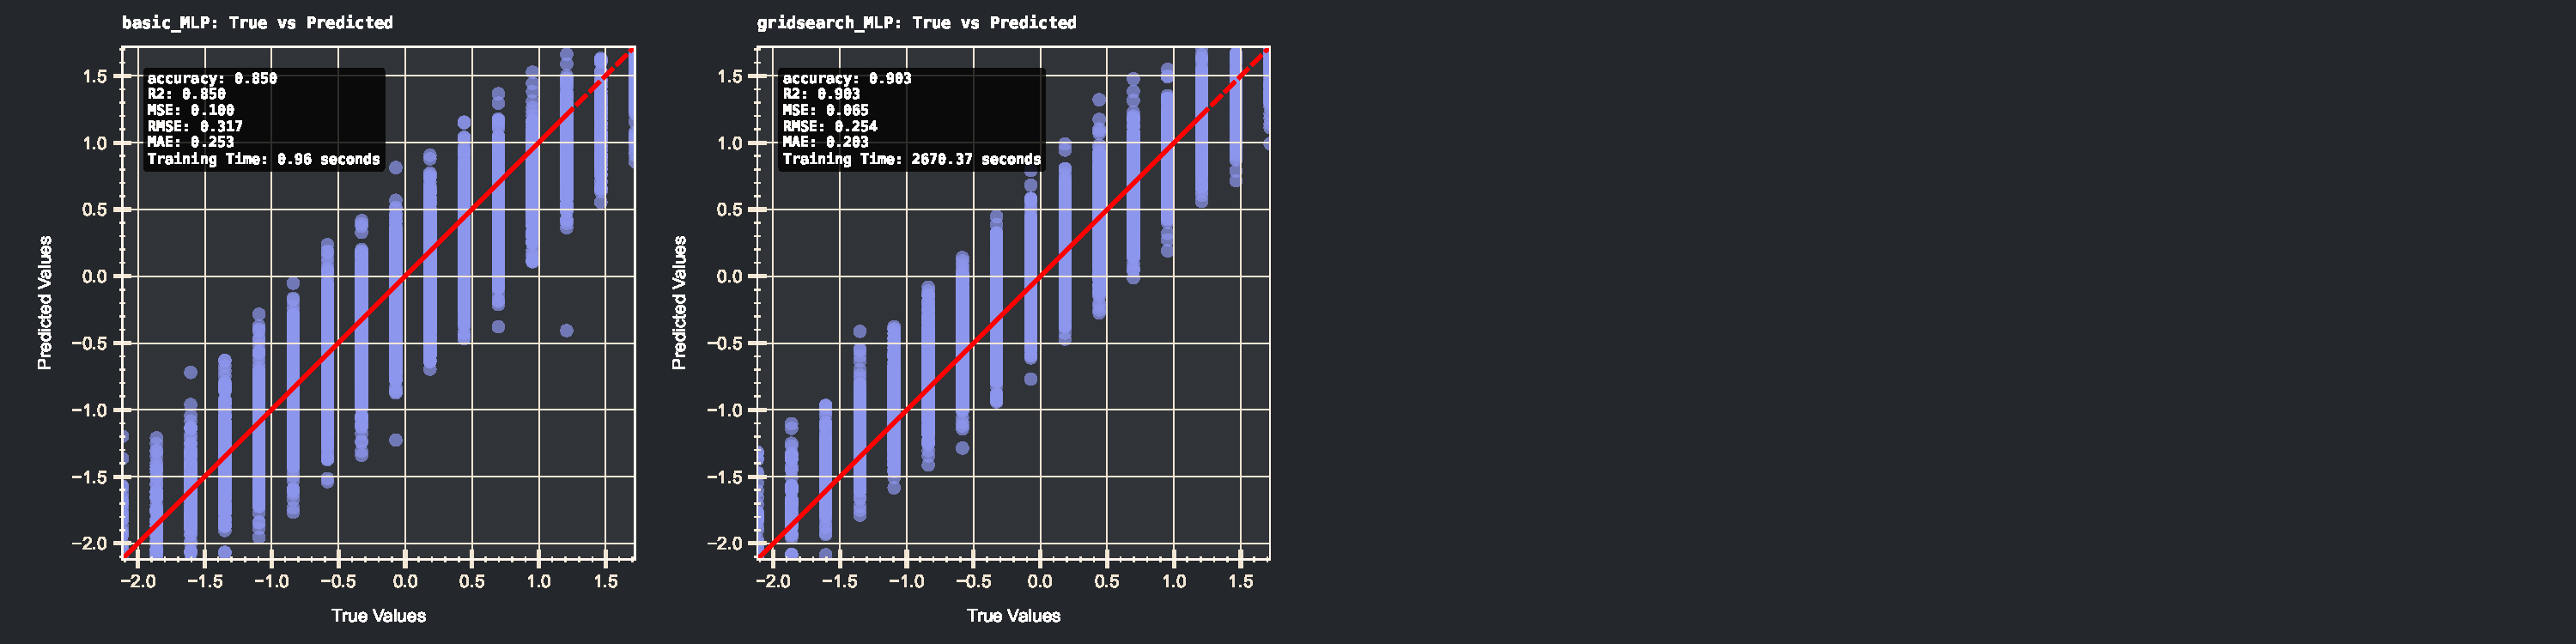
\includegraphics[width=6.5in,trim={0 0 25cm 0},clip]{../report/assets/nn1_best_models_result.pdf}    
\end{center}
These models did not perform as well as the previous ML models.
So i decided to use TensorFlow and Keras to customize the NN further.
I had already a pretty good idea on how the NN should like due to the previous step.
\lstinputlisting[style=independentpython,language=python,linerange={61-71,100-109}]{../chap_5_awakening_the_neural_mind/part_2_tensorflow.py}
This probably is the most simple NN you can find consisting of 1 input layer , 1 hidden layer , and 1 output layer.
The input layer has the same number of neurons as the number of features in the dataset that is given to it, the hidden layer has 32 neurons and the output layer has 1 neuron (because it's a regression task).
The first versions of the NN were not that good , sometimes overshooting and sometimes undershooting because i didn't use early stopping callback yet.

No Early Stopping:
\begin{center}
    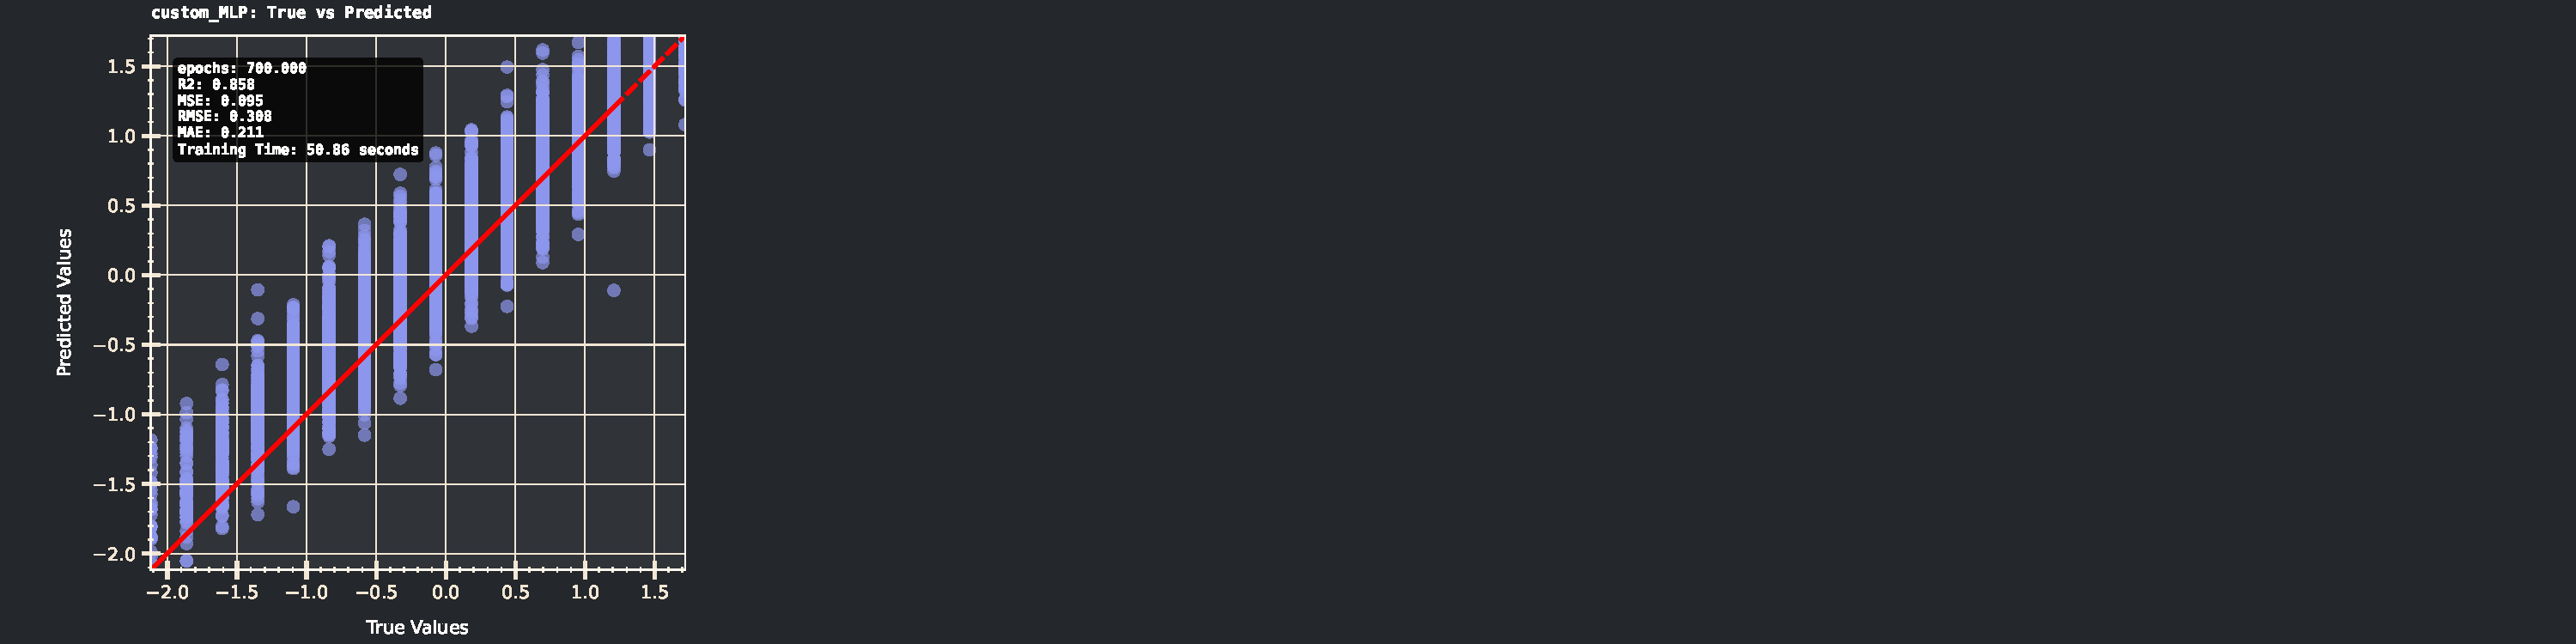
\includegraphics[width=4.5in,trim={0 0 30cm 0},clip]{../report/assets/nn4_best_models_result.pdf}
    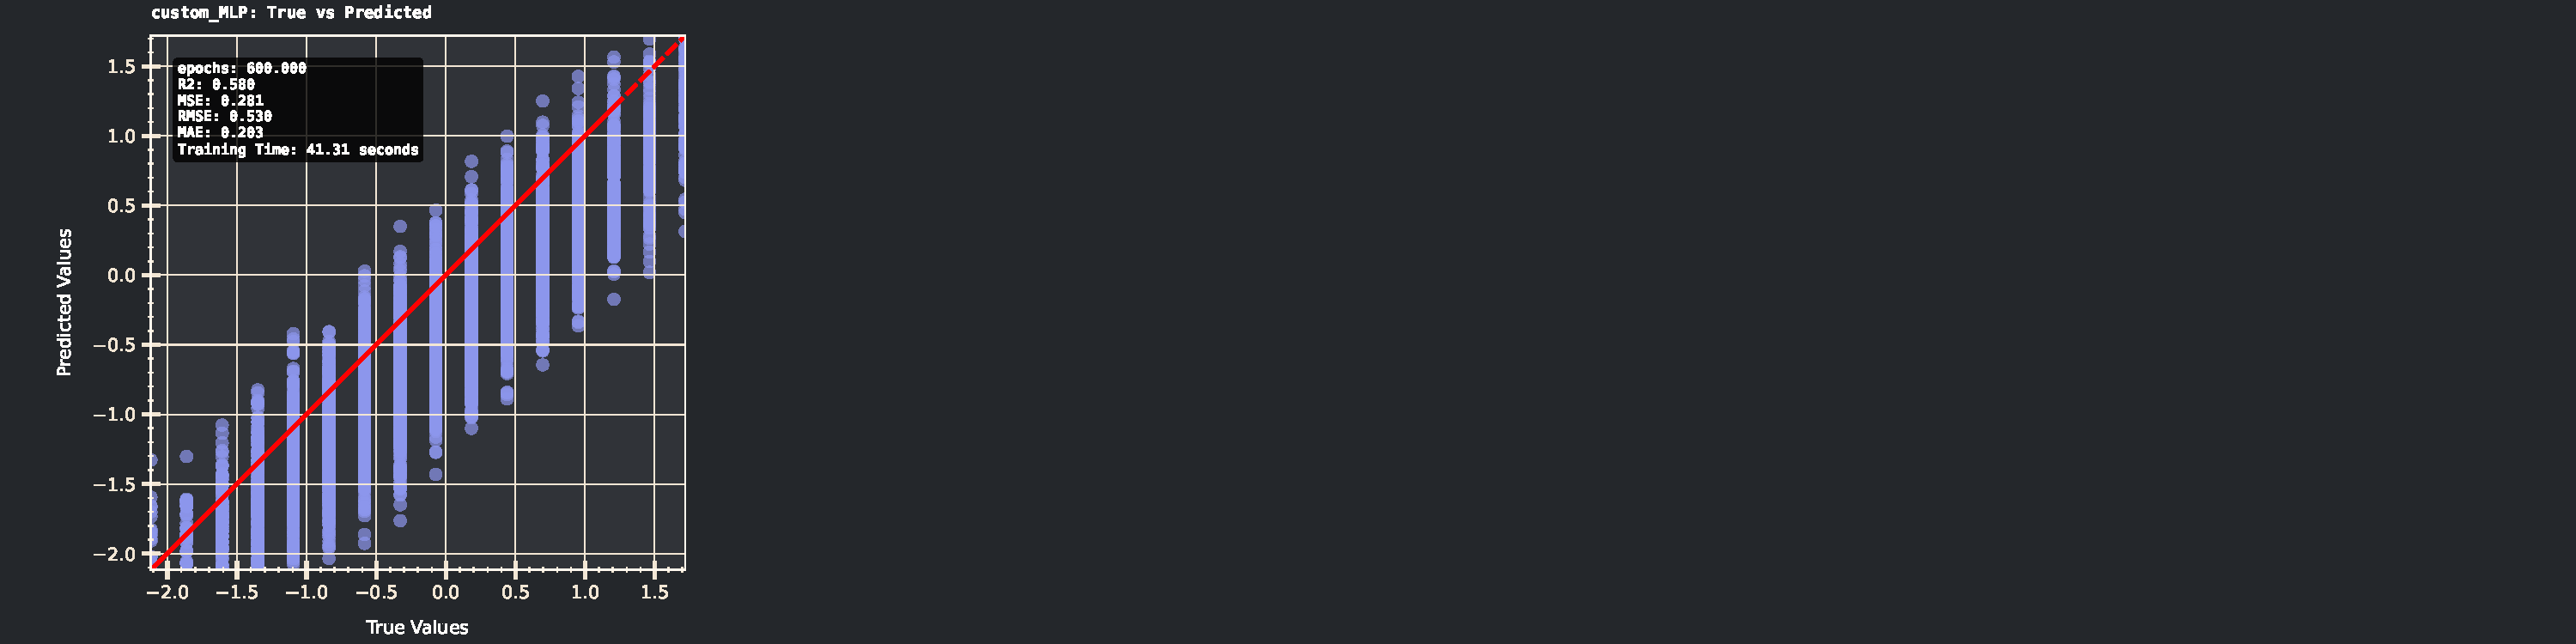
\includegraphics[width=4.5in,trim={0 0 30cm 0},clip]{../report/assets/nn5_best_models_result.pdf}
\end{center}
With Early Stopping:
\begin{center}
    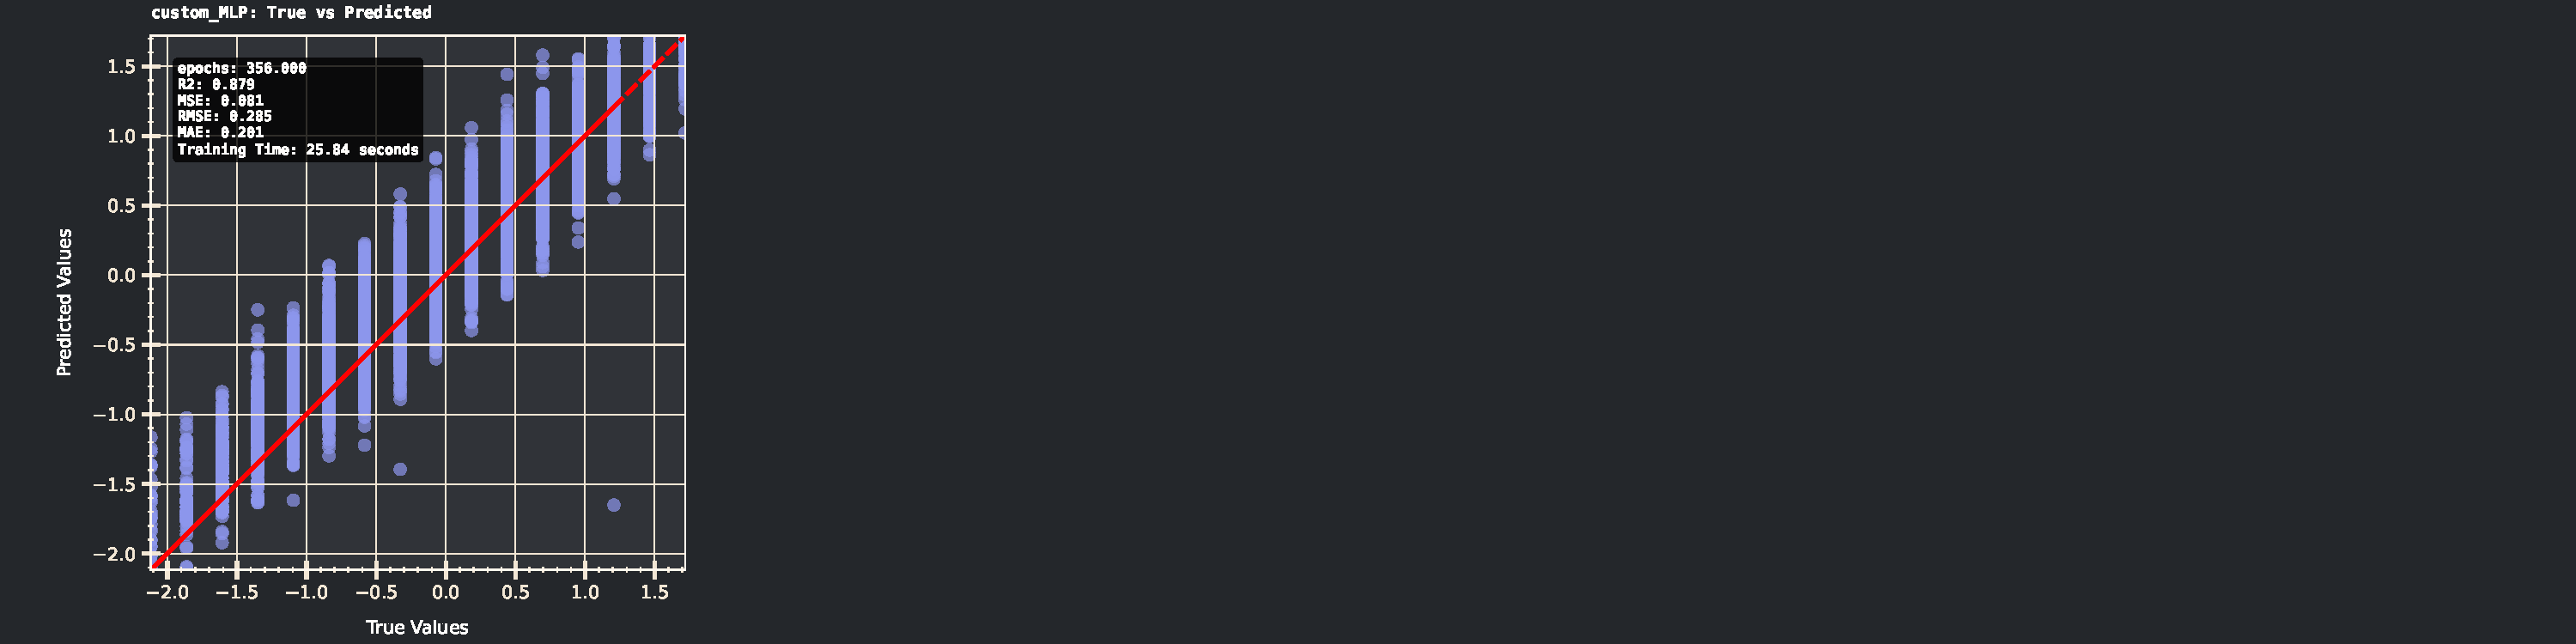
\includegraphics[width=4.5in,trim={0 0 30cm 0},clip]{../report/assets/nn8_best_models_result.pdf}
\end{center}

With early stopping the model was able to achieve a MSE of 0.081 on the test set. 
However the training time was significantly higher than the previous ML models and the MSE is still higher then these previous explored models.

My last attempt was to use the full data set to train the model and see if it would improve the performance of the model.
\begin{center}
    Full Dataset:
    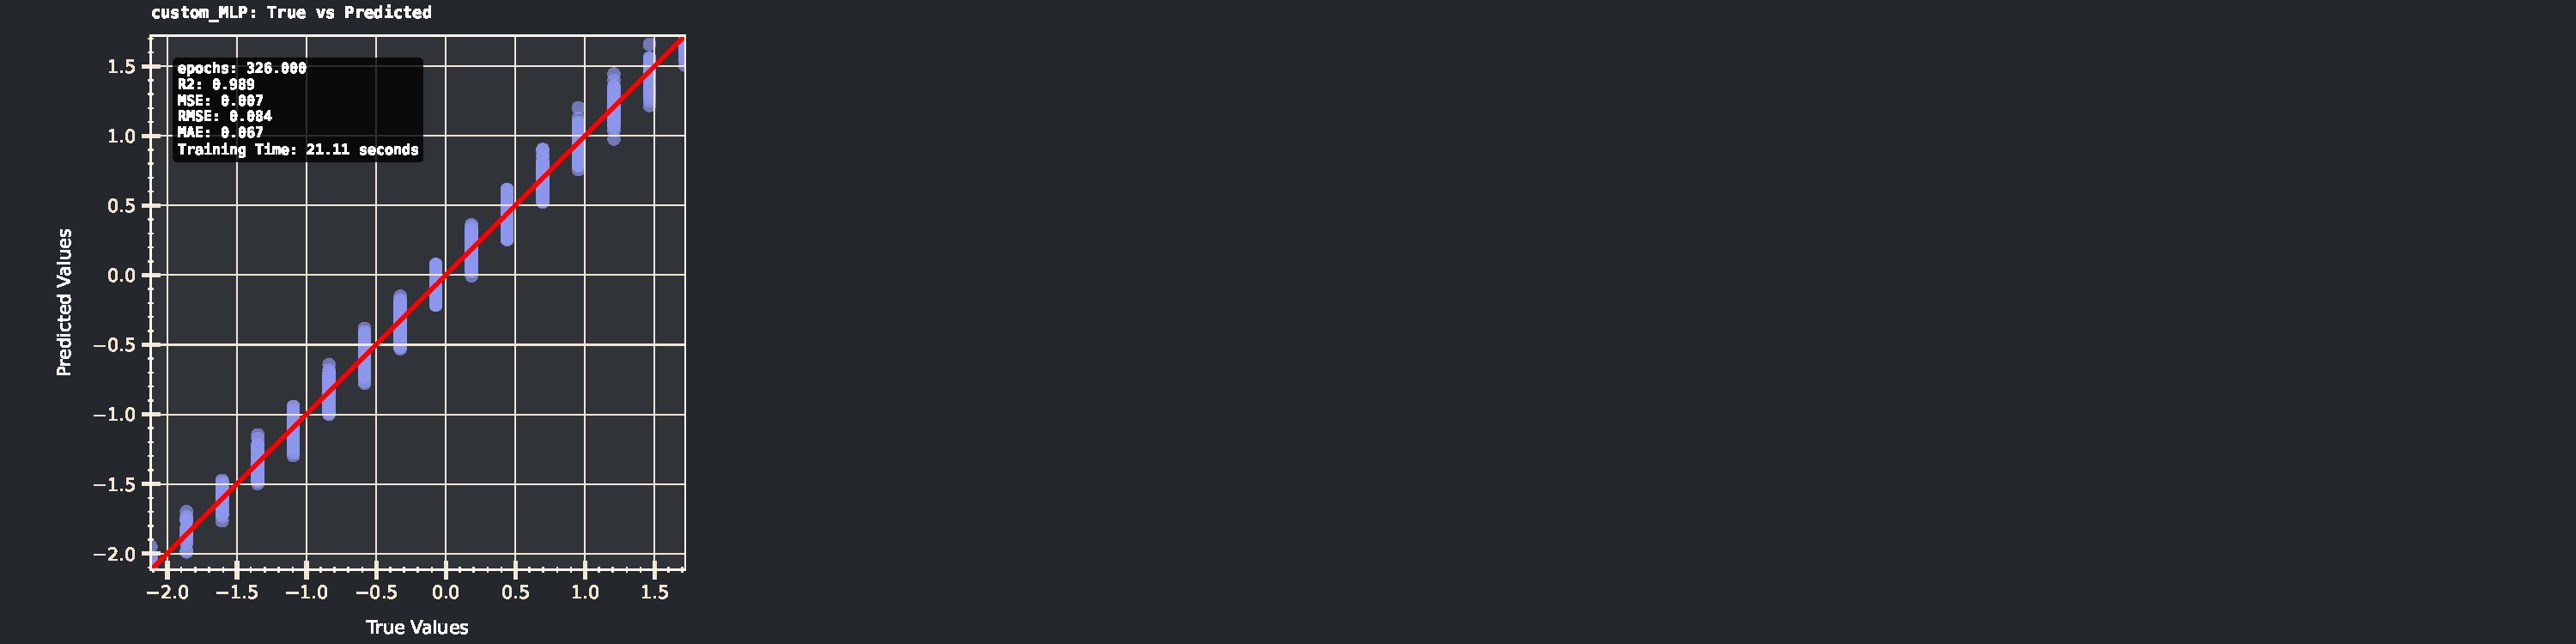
\includegraphics[width=6.5in,trim={0 0 30cm 0},clip]{../report/assets/nn9_best_models_result.pdf}
    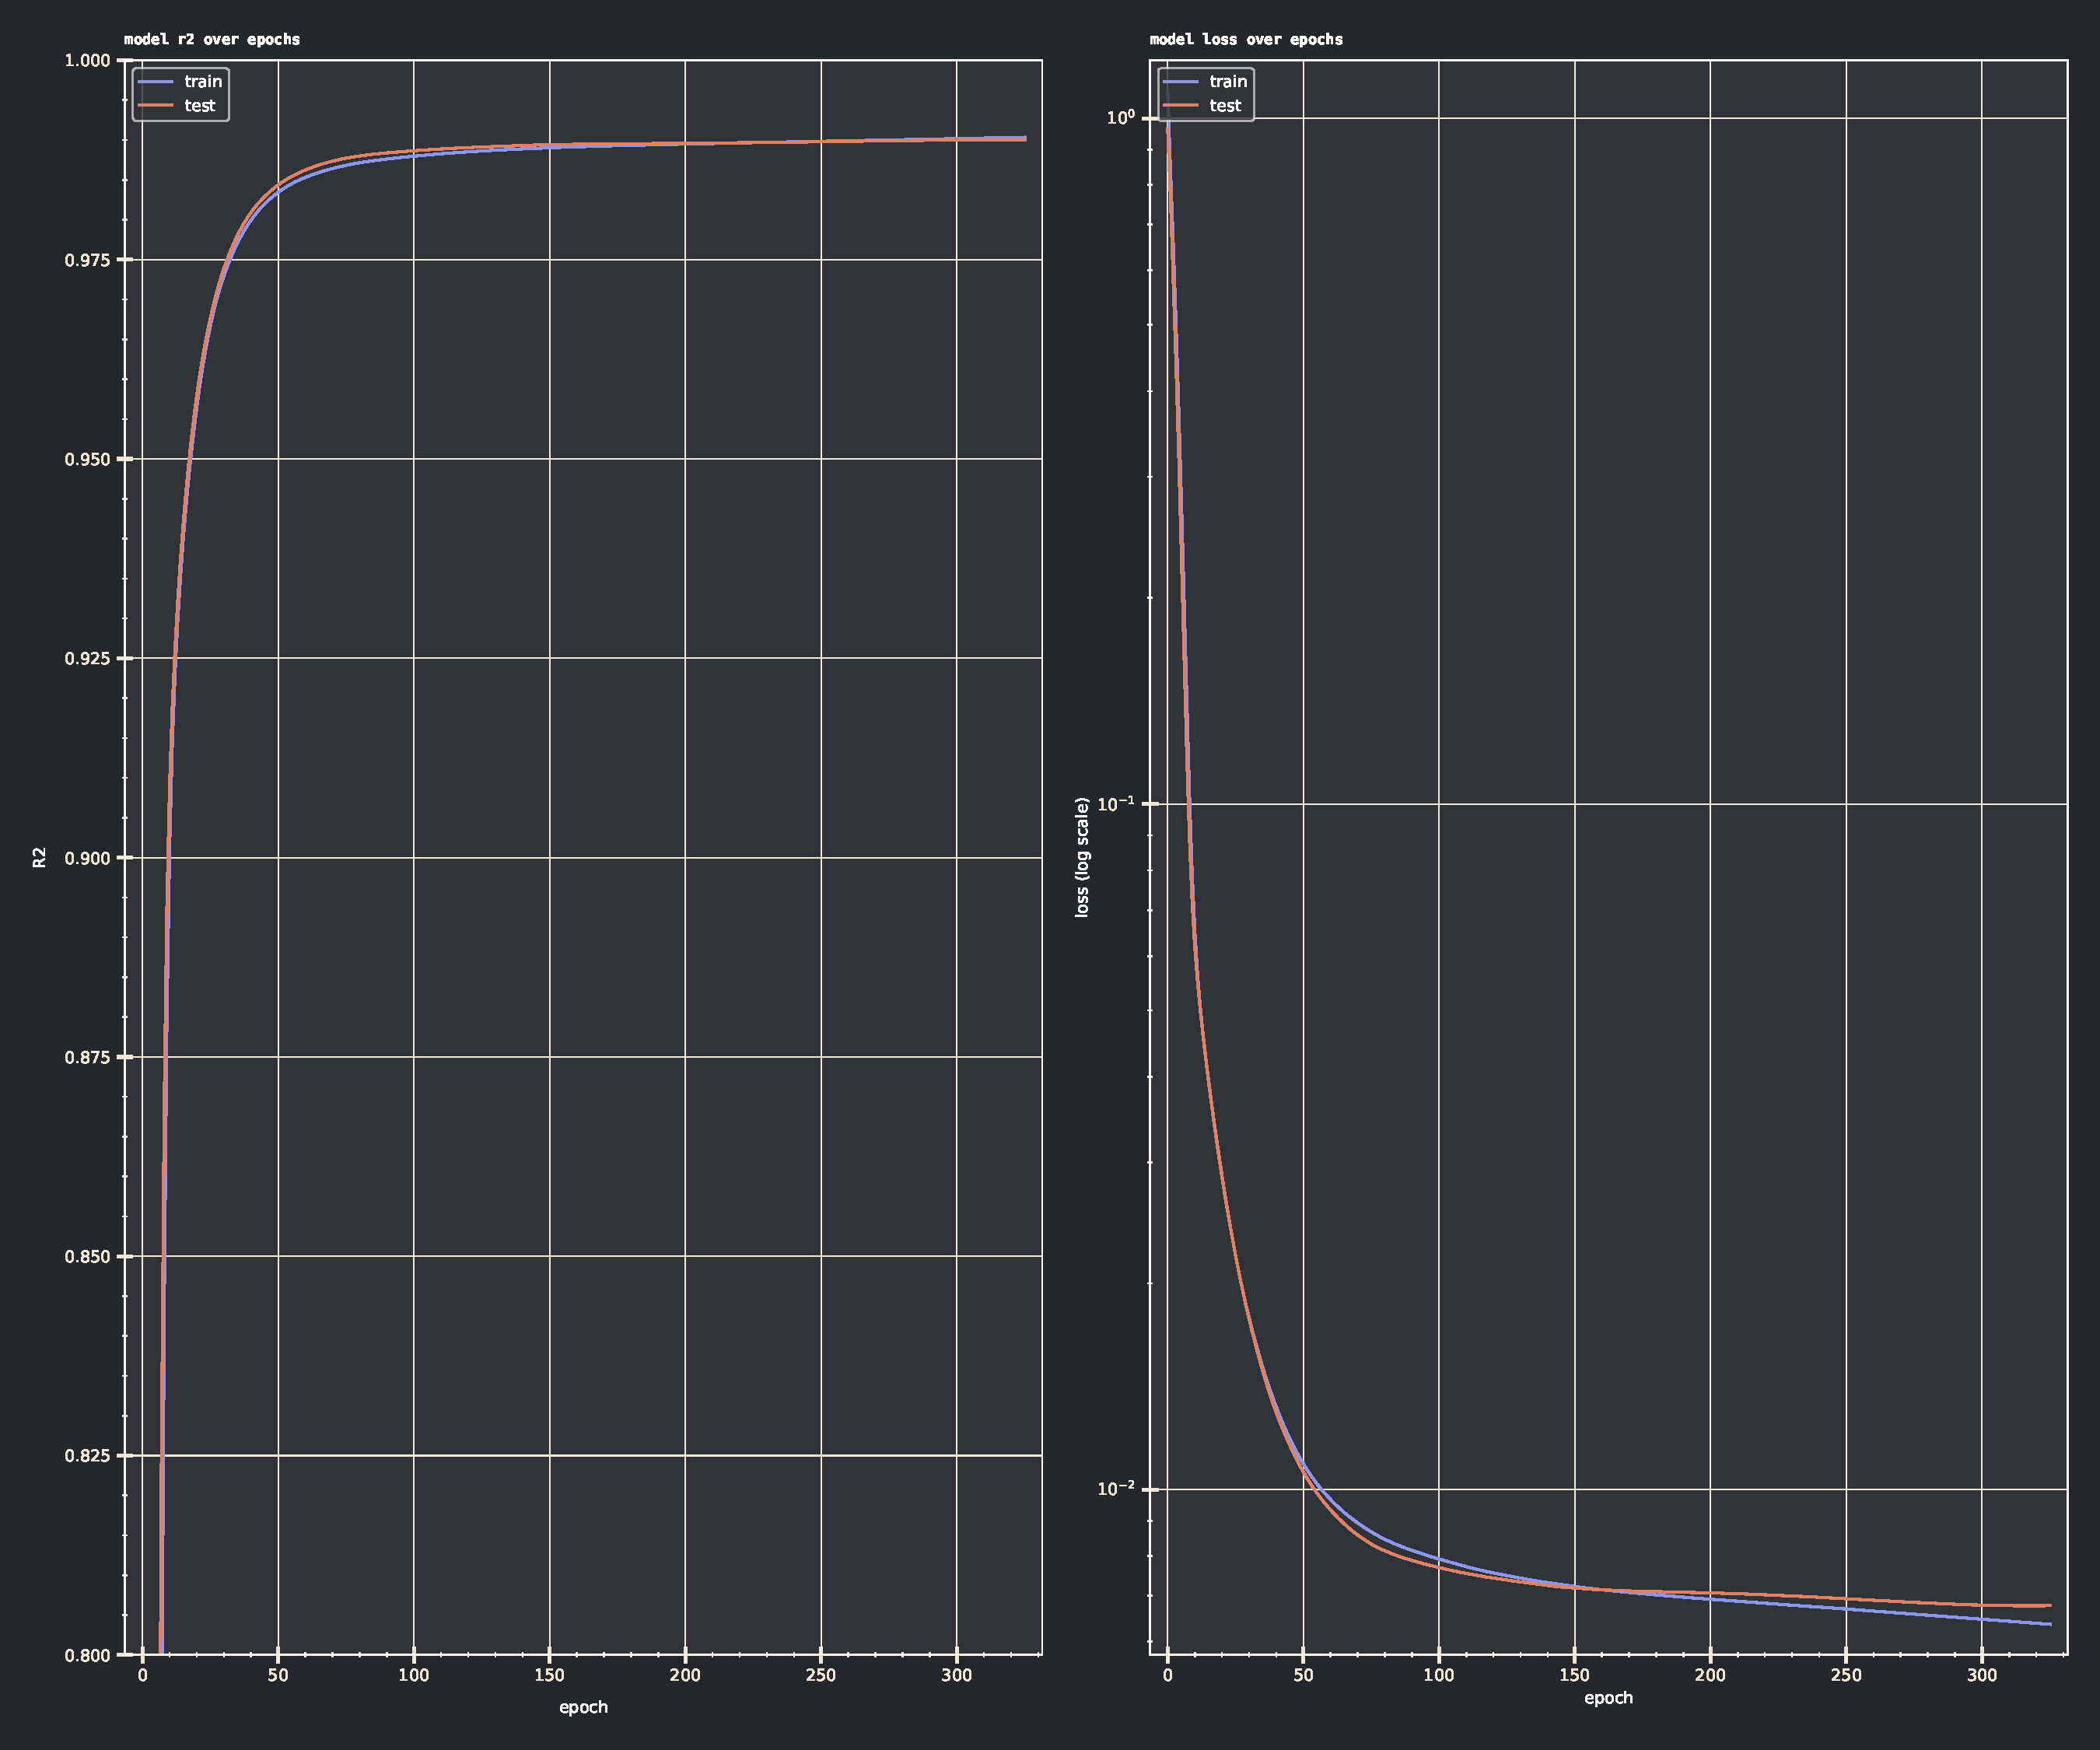
\includegraphics[width=6.5in]{../report/assets/nn9_nn_results.pdf}
\end{center}
Yeah this is probably the best model i could come up with, having a MSE of 0.00711 on the test set.
significantly outperforming the previous ML models and the previous NN models.
But again the training time was significantly higher than the previous ML models.
with a ratio of 
\begin{align}
    \textbf{t}_{NN} &= 0.00092 \text{ seconds} \\
    \textbf{t}_{LinearReggression} &= 21.10520 \text{ seconds} \\
    \text{Ratio} &= \frac{\textbf{t}_{LinearReggression}}{\textbf{t}_{NN}} = \frac{21.10520}{0.00092} \approx 22940.43
\end{align}
So the training time of the NN is about 22940 times higher than the training time of the Linear Regression model.

% SHAP =========================================================================================
\newpage
\section{SHAP}
\subsection{SHAP Analysis}
To understand the impact of each feature on the model's predictions, I used SHAP (SHapley Additive exPlanations) values.
SHAP values provide a way to explain the output of any machine learning model by assigning each feature an importance value for a particular prediction.

\subsection{SHAP Values Calculation}
I used the SHAP library to calculate the SHAP values for the best model (the Neural Network) and then visualized the results using a beeswarm plot.
\lstinputlisting[style=independentpython,language=python,linerange={59,61,65,73}]{../chap_6_cracking_the_black_box/part_1_shap.py}
\begin{center}
    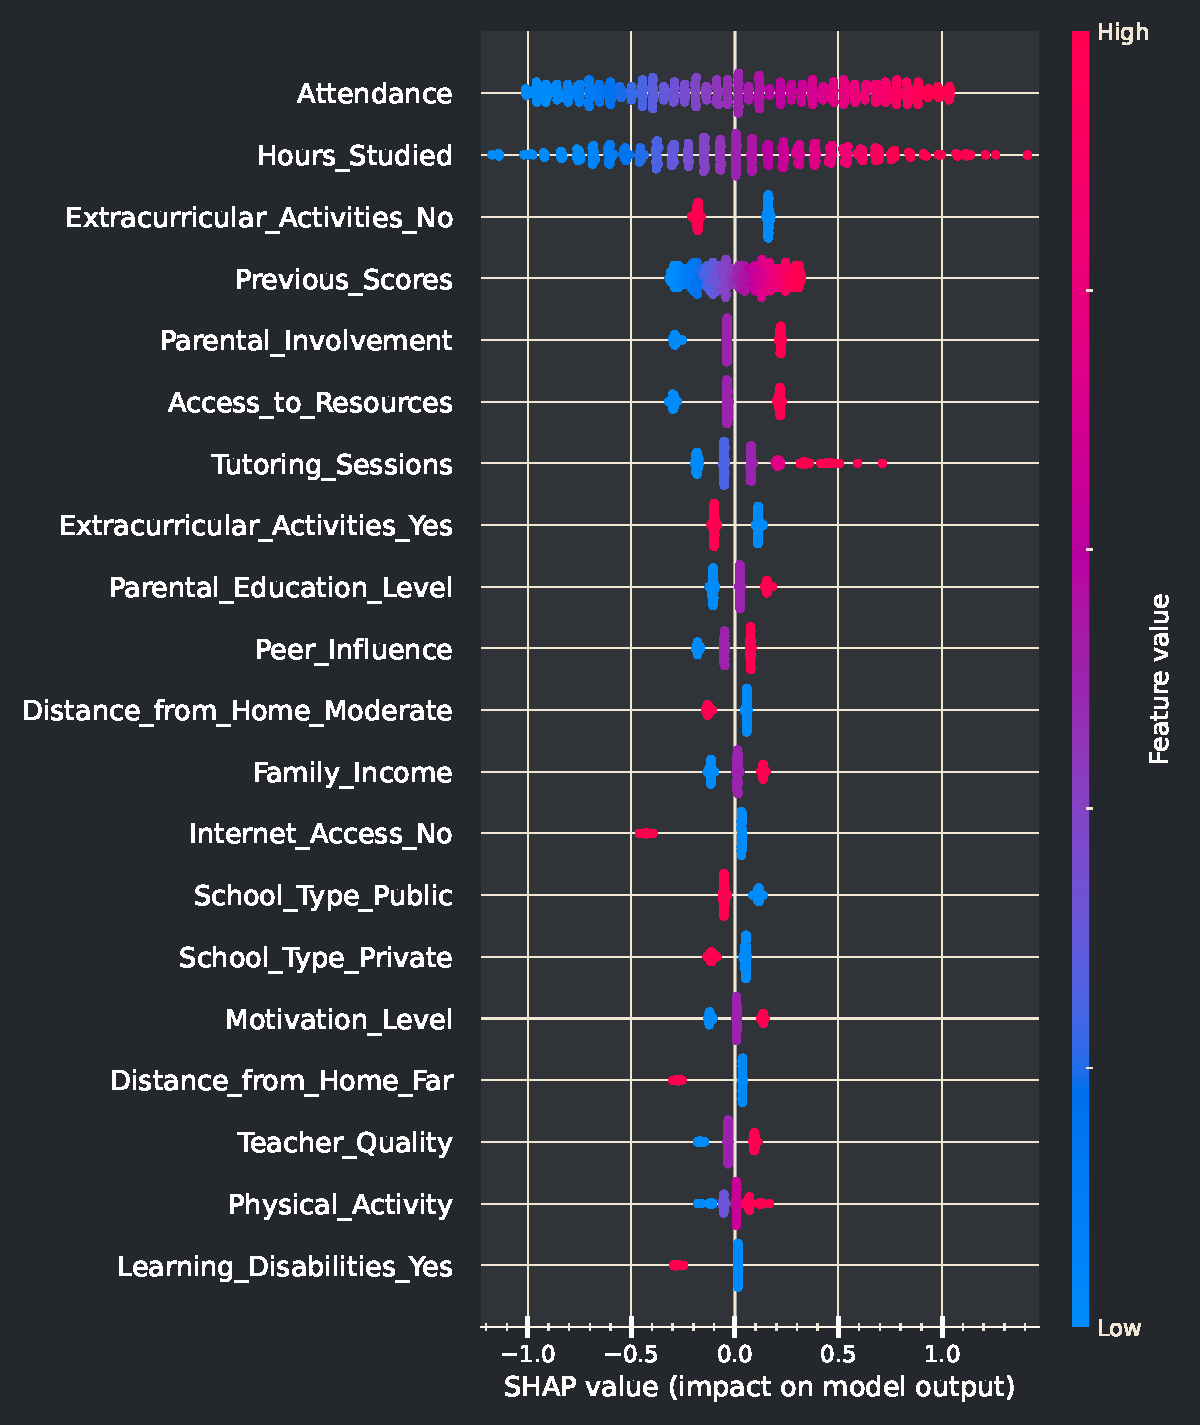
\includegraphics[width=5.5in]{../report/assets/SHAP_values_beeswarm.pdf}
\end{center}
What we can see here is how each feature contributes to the model's predictions.
The beeswarm plot shows the SHAP values for each feature, with the color indicating the feature value (red for high values, blue for low values).

% Final word ==========================================================================================
\newpage
\section{Conclusion}
I could conclude that the best model for this dataset is the Neural Network with a MSE of 0.00711 on the test set.
However the training time of the NN is significantly higher than the previous ML models, which makes it less suitable for this dataset.
The previous ML models were able to achieve a MSE of 0.064 on the test set, which is still a good result.
I could have used the whole dataset on the ML models and used PCA to reduce the dimensionality of the dataset, but i did not have the time to do so. 
Nor did i have the time to try different combination of features to see if it would improve the performance of the model.
In conclusion, the project was a success in terms of achieving the goal of building a machine learning model that can predict the students exam score based on the various factors provided in the dataset. 

\end{document}